%&latex
\NeedsTeXFormat{LaTeX2e}
%\documentstyle[makeidx]{cmmp}
\documentclass[10pt,a4paper,titlepage]{book}

\usepackage{astron}
\usepackage{psfig}
\usepackage{psfig,amssymb,alltt}
\usepackage{latexsym}
\usepackage{graphicx}
\graphicspath{{PS/}}
\usepackage{psfig}
\usepackage[english]{babel}
\usepackage{indentfirst}
\usepackage{amsmath}
\usepackage{makeidx}
% \usepackage{astron}
 
\pagestyle{headings}
% \pagenumbering{roman}
% \setcounter{page}{5}
\makeindex
\thispagestyle{empty}

\usepackage{psfig}
%\newcommand{\psdir}{/export/home/starck/Main/sadam/tex/report/FIG}
\newcommand{\psdir}{/Users/yassirmoudden/travail/programmes/MRS/doc}
% \psfigurepath{\psdir/mr1:\psdir/demo:\psdir/cours:\psdir/edge:\psdir/compress:\psdir/fractal:\psdir/detect:\psdir/book98:\psdir/entropy:\psdir/iso:\psdir/cours}
\psfigurepath{./PS}


\def\aa{{A\&A } }
\def\aj{{AJ} }
\def\apj{{ApJ\ }}
\def\va{{ Vistas in Astronomy}}
\def\pasp{{ PASP\ }}
 
\newcommand{\be}{\begin{eqnarray}}
\newcommand{\ee}{\end{eqnarray}}
\newcommand{\goto}{\rightarrow}
\newcommand{\bitem}{\begin{itemize}}
\newcommand{\eitem}{\end{itemize}}
\newcommand{\bR}{{\bf R}}
\newcommand{\eps}{{\epsilon}}
\newcommand{\cR}{{\cal R}}
\newcommand{\cQ}{{\cal Q}}
\newcommand{\bZ}{{\bf Z}}
\newcommand{\cM}{{\cal M}}
% \newcommand{\<}{\langle}
\renewcommand{\>}{\rangle}
% \newcommand{\qed}{\quad\hbox{\vrule width 4pt height 6pt depth 1.5pt}}
\newcommand{\cH}{{\cal H}}
\newcommand{\cL}{{\cal L}}

\newcommand{\tkle}{${\tilde \kappa}_l^{(E)}$}
\newcommand{\tklb}{${\tilde \kappa}_l^{(B)}$}

\newcommand{\com}[1]{{\large \bf[#1]}}
\newcommand{\lam}{\lambda}
\newcommand{\mmax}{\mathrm{max}}

\def\dom{\mathcal{D}}
\def\diag{\mathrm{diag}}
\def\trace{\mathrm{tr}}
\def\inv{^{-1}}
\def\adj{^\dagger }
\def\vect{\mathrm{vect}}
\def\ud{\mathrm{d}}
 

\def\projmw{MRS}
\def\defprojmw{Multi-Resolution on the Sphere}
\def\mrs{MRS }
\textwidth 16truecm
\textheight 22.5truecm
\hoffset -1.truecm
\voffset -1.5truecm
\evensidemargin 1.truecm
\oddsidemargin  1.truecm

% \makeindex
%% Psfig/TeX 
\def\PsfigVersion{1.9}
% dvips version
%
% All psfig/tex software, documentation, and related files
% in this distribution of psfig/tex are 
% Copyright 1987, 1988, 1991 Trevor J. Darrell
%
% Permission is granted for use and non-profit distribution of psfig/tex 
% providing that this notice is clearly maintained. The right to
% distribute any portion of psfig/tex for profit or as part of any commercial
% product is specifically reserved for the author(s) of that portion.
%
% *** Feel free to make local modifications of psfig as you wish,
% *** but DO NOT post any changed or modified versions of ``psfig''
% *** directly to the net. Send them to me and I'll try to incorporate
% *** them into future versions. If you want to take the psfig code 
% *** and make a new program (subject to the copyright above), distribute it, 
% *** (and maintain it) that's fine, just don't call it psfig.
%
% Bugs and improvements to trevor@media.mit.edu.
%
% Thanks to Greg Hager (GDH) and Ned Batchelder for their contributions
% to the original version of this project.
%
% Modified by J. Daniel Smith on 9 October 1990 to accept the
% %%BoundingBox: comment with or without a space after the colon.  Stole
% file reading code from Tom Rokicki's EPSF.TEX file (see below).
%
% More modifications by J. Daniel Smith on 29 March 1991 to allow the
% the included PostScript figure to be rotated.  The amount of
% rotation is specified by the "angle=" parameter of the \psfig command.
%
% Modified by Robert Russell on June 25, 1991 to allow users to specify
% .ps filenames which don't yet exist, provided they explicitly provide
% boundingbox information via the \psfig command. Note: This will only work
% if the "file=" parameter follows all four "bb???=" parameters in the
% command. This is due to the order in which psfig interprets these params.
%
%  3 Jul 1991	JDS	check if file already read in once
%  4 Sep 1991	JDS	fixed incorrect computation of rotated
%			bounding box
% 25 Sep 1991	GVR	expanded synopsis of \psfig
% 14 Oct 1991	JDS	\fbox code from LaTeX so \psdraft works with TeX
%			changed \typeout to \ps@typeout
% 17 Oct 1991	JDS	added \psscalefirst and \psrotatefirst
%

% From: gvr@cs.brown.edu (George V. Reilly)
%
% \psdraft	draws an outline box, but doesn't include the figure
%		in the DVI file.  Useful for previewing.
%
% \psfull	includes the figure in the DVI file (default).
%
% \psscalefirst width= or height= specifies the size of the figure
% 		before rotation.
% \psrotatefirst (default) width= or height= specifies the size of the
% 		 figure after rotation.  Asymetric figures will
% 		 appear to shrink.
%
% \psfigurepath#1	sets the path to search for the figure
%
% \psfig
% usage: \psfig{file=, figure=, height=, width=,
%			bbllx=, bblly=, bburx=, bbury=,
%			rheight=, rwidth=, clip=, angle=, silent=}
%
%	"file" is the filename.  If no path name is specified and the
%		file is not found in the current directory,
%		it will be looked for in directory \psfigurepath.
%	"figure" is a synonym for "file".
%	By default, the width and height of the figure are taken from
%		the BoundingBox of the figure.
%	If "width" is specified, the figure is scaled so that it has
%		the specified width.  Its height changes proportionately.
%	If "height" is specified, the figure is scaled so that it has
%		the specified height.  Its width changes proportionately.
%	If both "width" and "height" are specified, the figure is scaled
%		anamorphically.
%	"bbllx", "bblly", "bburx", and "bbury" control the PostScript
%		BoundingBox.  If these four values are specified
%               *before* the "file" option, the PSFIG will not try to
%               open the PostScript file.
%	"rheight" and "rwidth" are the reserved height and width
%		of the figure, i.e., how big TeX actually thinks
%		the figure is.  They default to "width" and "height".
%	The "clip" option ensures that no portion of the figure will
%		appear outside its BoundingBox.  "clip=" is a switch and
%		takes no value, but the `=' must be present.
%	The "angle" option specifies the angle of rotation (degrees, ccw).
%	The "silent" option makes \psfig work silently.
%

% check to see if macros already loaded in (maybe some other file says
% "\input psfig") ...
\ifx\undefined\psfig\else\endinput\fi

%
% from a suggestion by eijkhout@csrd.uiuc.edu to allow
% loading as a style file. Changed to avoid problems
% with amstex per suggestion by jbence@math.ucla.edu

\let\LaTeXAtSign=\@
\let\@=\relax
\edef\psfigRestoreAt{\catcode`\@=\number\catcode`@\relax}
%\edef\psfigRestoreAt{\catcode`@=\number\catcode`@\relax}
\catcode`\@=11\relax
\newwrite\@unused
\def\ps@typeout#1{{\let\protect\string\immediate\write\@unused{#1}}}
\ps@typeout{psfig/tex \PsfigVersion}

%% Here's how you define your figure path.  Should be set up with null
%% default and a user useable definition.

\def\figurepath{./}
\def\psfigurepath#1{\edef\figurepath{#1}}

%
% @psdo control structure -- similar to Latex @for.
% I redefined these with different names so that psfig can
% be used with TeX as well as LaTeX, and so that it will not 
% be vunerable to future changes in LaTeX's internal
% control structure,
%
\def\@nnil{\@nil}
\def\@empty{}
\def\@psdonoop#1\@@#2#3{}
\def\@psdo#1:=#2\do#3{\edef\@psdotmp{#2}\ifx\@psdotmp\@empty \else
    \expandafter\@psdoloop#2,\@nil,\@nil\@@#1{#3}\fi}
\def\@psdoloop#1,#2,#3\@@#4#5{\def#4{#1}\ifx #4\@nnil \else
       #5\def#4{#2}\ifx #4\@nnil \else#5\@ipsdoloop #3\@@#4{#5}\fi\fi}
\def\@ipsdoloop#1,#2\@@#3#4{\def#3{#1}\ifx #3\@nnil 
       \let\@nextwhile=\@psdonoop \else
      #4\relax\let\@nextwhile=\@ipsdoloop\fi\@nextwhile#2\@@#3{#4}}
\def\@tpsdo#1:=#2\do#3{\xdef\@psdotmp{#2}\ifx\@psdotmp\@empty \else
    \@tpsdoloop#2\@nil\@nil\@@#1{#3}\fi}
\def\@tpsdoloop#1#2\@@#3#4{\def#3{#1}\ifx #3\@nnil 
       \let\@nextwhile=\@psdonoop \else
      #4\relax\let\@nextwhile=\@tpsdoloop\fi\@nextwhile#2\@@#3{#4}}
% 
% \fbox is defined in latex.tex; so if \fbox is undefined, assume that
% we are not in LaTeX.
% Perhaps this could be done better???
\ifx\undefined\fbox
% \fbox code from modified slightly from LaTeX
\newdimen\fboxrule
\newdimen\fboxsep
\newdimen\ps@tempdima
\newbox\ps@tempboxa
\fboxsep = 3pt
\fboxrule = .4pt
\long\def\fbox#1{\leavevmode\setbox\ps@tempboxa\hbox{#1}\ps@tempdima\fboxrule
    \advance\ps@tempdima \fboxsep \advance\ps@tempdima \dp\ps@tempboxa
   \hbox{\lower \ps@tempdima\hbox
  {\vbox{\hrule height \fboxrule
          \hbox{\vrule width \fboxrule \hskip\fboxsep
          \vbox{\vskip\fboxsep \box\ps@tempboxa\vskip\fboxsep}\hskip 
                 \fboxsep\vrule width \fboxrule}
                 \hrule height \fboxrule}}}}
\fi
%
%%%%%%%%%%%%%%%%%%%%%%%%%%%%%%%%%%%%%%%%%%%%%%%%%%%%%%%%%%%%%%%%%%%
% file reading stuff from epsf.tex
%   EPSF.TEX macro file:
%   Written by Tomas Rokicki of Radical Eye Software, 29 Mar 1989.
%   Revised by Don Knuth, 3 Jan 1990.
%   Revised by Tomas Rokicki to accept bounding boxes with no
%      space after the colon, 18 Jul 1990.
%   Portions modified/removed for use in PSFIG package by
%      J. Daniel Smith, 9 October 1990.
%
\newread\ps@stream
\newif\ifnot@eof       % continue looking for the bounding box?
\newif\if@noisy        % report what you're making?
\newif\if@atend        % %%BoundingBox: has (at end) specification
\newif\if@psfile       % does this look like a PostScript file?
%
% PostScript files should start with `%!'
%
{\catcode`\%=12\global\gdef\epsf@start{%!}}
\def\epsf@PS{PS}
%
\def\epsf@getbb#1{%
%
%   The first thing we need to do is to open the
%   PostScript file, if possible.
%
\openin\ps@stream=#1
\ifeof\ps@stream\ps@typeout{Error, File #1 not found}\else
%
%   Okay, we got it. Now we'll scan lines until we find one that doesn't
%   start with %. We're looking for the bounding box comment.
%
   {\not@eoftrue \chardef\other=12
    \def\do##1{\catcode`##1=\other}\dospecials \catcode`\ =10
    \loop
       \if@psfile
	  \read\ps@stream to \epsf@fileline
       \else{
	  \obeyspaces
          \read\ps@stream to \epsf@tmp\global\let\epsf@fileline\epsf@tmp}
       \fi
       \ifeof\ps@stream\not@eoffalse\else
%
%   Check the first line for `%!'.  Issue a warning message if its not
%   there, since the file might not be a PostScript file.
%
       \if@psfile\else
       \expandafter\epsf@test\epsf@fileline:. \\%
       \fi
%
%   We check to see if the first character is a % sign;
%   if so, we look further and stop only if the line begins with
%   `%%BoundingBox:' and the `(atend)' specification was not found.
%   That is, the only way to stop is when the end of file is reached,
%   or a `%%BoundingBox: llx lly urx ury' line is found.
%
          \expandafter\epsf@aux\epsf@fileline:. \\%
       \fi
   \ifnot@eof\repeat
   }\closein\ps@stream\fi}%
%
% This tests if the file we are reading looks like a PostScript file.
%
\long\def\epsf@test#1#2#3:#4\\{\def\epsf@testit{#1#2}
			\ifx\epsf@testit\epsf@start\else
\ps@typeout{Warning! File does not start with `\epsf@start'.  It may not be a PostScript file.}
			\fi
			\@psfiletrue} % don't test after 1st line
%
%   We still need to define the tricky \epsf@aux macro. This requires
%   a couple of magic constants for comparison purposes.
%
{\catcode`\%=12\global\let\epsf@percent=%\global\def\epsf@bblit{%BoundingBox}}
%
%
%   So we're ready to check for `%BoundingBox:' and to grab the
%   values if they are found.  We continue searching if `(at end)'
%   was found after the `%BoundingBox:'.
%
\long\def\epsf@aux#1#2:#3\\{\ifx#1\epsf@percent
   \def\epsf@testit{#2}\ifx\epsf@testit\epsf@bblit
	\@atendfalse
        \epsf@atend #3 . \\%
	\if@atend	
	   \if@verbose{
		\ps@typeout{psfig: found `(atend)'; continuing search}
	   }\fi
        \else
        \epsf@grab #3 . . . \\%
        \not@eoffalse
        \global\no@bbfalse
        \fi
   \fi\fi}%
%
%   Here we grab the values and stuff them in the appropriate definitions.
%
\def\epsf@grab #1 #2 #3 #4 #5\\{%
   \global\def\epsf@llx{#1}\ifx\epsf@llx\empty
      \epsf@grab #2 #3 #4 #5 .\\\else
   \global\def\epsf@lly{#2}%
   \global\def\epsf@urx{#3}\global\def\epsf@ury{#4}\fi}%
%
% Determine if the stuff following the %%BoundingBox is `(atend)'
% J. Daniel Smith.  Copied from \epsf@grab above.
%
\def\epsf@atendlit{(atend)} 
\def\epsf@atend #1 #2 #3\\{%
   \def\epsf@tmp{#1}\ifx\epsf@tmp\empty
      \epsf@atend #2 #3 .\\\else
   \ifx\epsf@tmp\epsf@atendlit\@atendtrue\fi\fi}


% End of file reading stuff from epsf.tex
%%%%%%%%%%%%%%%%%%%%%%%%%%%%%%%%%%%%%%%%%%%%%%%%%%%%%%%%%%%%%%%%%%%

%%%%%%%%%%%%%%%%%%%%%%%%%%%%%%%%%%%%%%%%%%%%%%%%%%%%%%%%%%%%%%%%%%%
% trigonometry stuff from "trig.tex"
\chardef\psletter = 11 % won't conflict with \begin{letter} now...
\chardef\other = 12

\newif \ifdebug %%% turn me on to see TeX hard at work ...
\newif\ifc@mpute %%% don't need to compute some values
\c@mputetrue % but assume that we do

\let\then = \relax
\def\r@dian{pt }
\let\r@dians = \r@dian
\let\dimensionless@nit = \r@dian
\let\dimensionless@nits = \dimensionless@nit
\def\internal@nit{sp }
\let\internal@nits = \internal@nit
\newif\ifstillc@nverging
\def \Mess@ge #1{\ifdebug \then \message {#1} \fi}

{ %%% Things that need abnormal catcodes %%%
	\catcode `\@ = \psletter
	\gdef \nodimen {\expandafter \n@dimen \the \dimen}
	\gdef \term #1 #2 #3%
	       {\edef \t@ {\the #1}%%% freeze parameter 1 (count, by value)
		\edef \t@@ {\expandafter \n@dimen \the #2\r@dian}%
				   %%% freeze parameter 2 (dimen, by value)
		\t@rm {\t@} {\t@@} {#3}%
	       }
	\gdef \t@rm #1 #2 #3%
	       {{%
		\count 0 = 0
		\dimen 0 = 1 \dimensionless@nit
		\dimen 2 = #2\relax
		\Mess@ge {Calculating term #1 of \nodimen 2}%
		\loop
		\ifnum	\count 0 < #1
		\then	\advance \count 0 by 1
			\Mess@ge {Iteration \the \count 0 \space}%
			\Multiply \dimen 0 by {\dimen 2}%
			\Mess@ge {After multiplication, term = \nodimen 0}%
			\Divide \dimen 0 by {\count 0}%
			\Mess@ge {After division, term = \nodimen 0}%
		\repeat
		\Mess@ge {Final value for term #1 of 
				\nodimen 2 \space is \nodimen 0}%
		\xdef \Term {#3 = \nodimen 0 \r@dians}%
		\aftergroup \Term
	       }}
	\catcode `\p = \other
	\catcode `\t = \other
	\gdef \n@dimen #1pt{#1} %%% throw away the ``pt''
}

\def \Divide #1by #2{\divide #1 by #2} %%% just a synonym

\def \Multiply #1by #2%%% allows division of a dimen by a dimen
       {{%%% should really freeze parameter 2 (dimen, passed by value)
	\count 0 = #1\relax
	\count 2 = #2\relax
	\count 4 = 65536
	\Mess@ge {Before scaling, count 0 = \the \count 0 \space and
			count 2 = \the \count 2}%
	\ifnum	\count 0 > 32767 %%% do our best to avoid overflow
	\then	\divide \count 0 by 4
		\divide \count 4 by 4
	\else	\ifnum	\count 0 < -32767
		\then	\divide \count 0 by 4
			\divide \count 4 by 4
		\else
		\fi
	\fi
	\ifnum	\count 2 > 32767 %%% while retaining reasonable accuracy
	\then	\divide \count 2 by 4
		\divide \count 4 by 4
	\else	\ifnum	\count 2 < -32767
		\then	\divide \count 2 by 4
			\divide \count 4 by 4
		\else
		\fi
	\fi
	\multiply \count 0 by \count 2
	\divide \count 0 by \count 4
	\xdef \product {#1 = \the \count 0 \internal@nits}%
	\aftergroup \product
       }}

\def\r@duce{\ifdim\dimen0 > 90\r@dian \then   % sin(x+90) = sin(180-x)
		\multiply\dimen0 by -1
		\advance\dimen0 by 180\r@dian
		\r@duce
	    \else \ifdim\dimen0 < -90\r@dian \then  % sin(-x) = sin(360+x)
		\advance\dimen0 by 360\r@dian
		\r@duce
		\fi
	    \fi}

\def\Sine#1%
       {{%
	\dimen 0 = #1 \r@dian
	\r@duce
	\ifdim\dimen0 = -90\r@dian \then
	   \dimen4 = -1\r@dian
	   \c@mputefalse
	\fi
	\ifdim\dimen0 = 90\r@dian \then
	   \dimen4 = 1\r@dian
	   \c@mputefalse
	\fi
	\ifdim\dimen0 = 0\r@dian \then
	   \dimen4 = 0\r@dian
	   \c@mputefalse
	\fi
%
	\ifc@mpute \then
        	% convert degrees to radians
		\divide\dimen0 by 180
		\dimen0=3.141592654\dimen0
%
		\dimen 2 = 3.1415926535897963\r@dian %%% a well-known constant
		\divide\dimen 2 by 2 %%% we only deal with -pi/2 : pi/2
		\Mess@ge {Sin: calculating Sin of \nodimen 0}%
		\count 0 = 1 %%% see power-series expansion for sine
		\dimen 2 = 1 \r@dian %%% ditto
		\dimen 4 = 0 \r@dian %%% ditto
		\loop
			\ifnum	\dimen 2 = 0 %%% then we've done
			\then	\stillc@nvergingfalse 
			\else	\stillc@nvergingtrue
			\fi
			\ifstillc@nverging %%% then calculate next term
			\then	\term {\count 0} {\dimen 0} {\dimen 2}%
				\advance \count 0 by 2
				\count 2 = \count 0
				\divide \count 2 by 2
				\ifodd	\count 2 %%% signs alternate
				\then	\advance \dimen 4 by \dimen 2
				\else	\advance \dimen 4 by -\dimen 2
				\fi
		\repeat
	\fi		
			\xdef \sine {\nodimen 4}%
       }}

% Now the Cosine can be calculated easily by calling \Sine
\def\Cosine#1{\ifx\sine\UnDefined\edef\Savesine{\relax}\else
		             \edef\Savesine{\sine}\fi
	{\dimen0=#1\r@dian\advance\dimen0 by 90\r@dian
	 \Sine{\nodimen 0}
	 \xdef\cosine{\sine}
	 \xdef\sine{\Savesine}}}	      
% end of trig stuff
%%%%%%%%%%%%%%%%%%%%%%%%%%%%%%%%%%%%%%%%%%%%%%%%%%%%%%%%%%%%%%%%%%%%

\def\psdraft{
	\def\@psdraft{0}
	%\ps@typeout{draft level now is \@psdraft \space . }
}
\def\psfull{
	\def\@psdraft{100}
	%\ps@typeout{draft level now is \@psdraft \space . }
}

\psfull

\newif\if@scalefirst
\def\psscalefirst{\@scalefirsttrue}
\def\psrotatefirst{\@scalefirstfalse}
\psrotatefirst

\newif\if@draftbox
\def\psnodraftbox{
	\@draftboxfalse
}
\def\psdraftbox{
	\@draftboxtrue
}
\@draftboxtrue

\newif\if@prologfile
\newif\if@postlogfile
\def\pssilent{
	\@noisyfalse
}
\def\psnoisy{
	\@noisytrue
}
\psnoisy
%%% These are for the option list.
%%% A specification of the form a = b maps to calling \@p@@sa{b}
\newif\if@bbllx
\newif\if@bblly
\newif\if@bburx
\newif\if@bbury
\newif\if@height
\newif\if@width
\newif\if@rheight
\newif\if@rwidth
\newif\if@angle
\newif\if@clip
\newif\if@verbose
\def\@p@@sclip#1{\@cliptrue}


\newif\if@decmpr

%%% GDH 7/26/87 -- changed so that it first looks in the local directory,
%%% then in a specified global directory for the ps file.
%%% RPR 6/25/91 -- changed so that it defaults to user-supplied name if
%%% boundingbox info is specified, assuming graphic will be created by
%%% print time.
%%% TJD 10/19/91 -- added bbfile vs. file distinction, and @decmpr flag

\def\@p@@sfigure#1{\def\@p@sfile{null}\def\@p@sbbfile{null}
	        \openin1=#1.bb
		\ifeof1\closein1
	        	\openin1=\figurepath#1.bb
			\ifeof1\closein1
			        \openin1=#1
				\ifeof1\closein1%
				       \openin1=\figurepath#1
					\ifeof1
					   \ps@typeout{Error, File #1 not found}
						\if@bbllx\if@bblly
				   		\if@bburx\if@bbury
			      				\def\@p@sfile{#1}%
			      				\def\@p@sbbfile{#1}%
							\@decmprfalse
				  	   	\fi\fi\fi\fi
					\else\closein1
				    		\def\@p@sfile{\figurepath#1}%
				    		\def\@p@sbbfile{\figurepath#1}%
						\@decmprfalse
	                       		\fi%
			 	\else\closein1%
					\def\@p@sfile{#1}
					\def\@p@sbbfile{#1}
					\@decmprfalse
			 	\fi
			\else
				\def\@p@sfile{\figurepath#1}
				\def\@p@sbbfile{\figurepath#1.bb}
				\@decmprtrue
			\fi
		\else
			\def\@p@sfile{#1}
			\def\@p@sbbfile{#1.bb}
			\@decmprtrue
		\fi}

\def\@p@@sfile#1{\@p@@sfigure{#1}}

\def\@p@@sbbllx#1{
		%\ps@typeout{bbllx is #1}
		\@bbllxtrue
		\dimen100=#1
		\edef\@p@sbbllx{\number\dimen100}
}
\def\@p@@sbblly#1{
		%\ps@typeout{bblly is #1}
		\@bbllytrue
		\dimen100=#1
		\edef\@p@sbblly{\number\dimen100}
}
\def\@p@@sbburx#1{
		%\ps@typeout{bburx is #1}
		\@bburxtrue
		\dimen100=#1
		\edef\@p@sbburx{\number\dimen100}
}
\def\@p@@sbbury#1{
		%\ps@typeout{bbury is #1}
		\@bburytrue
		\dimen100=#1
		\edef\@p@sbbury{\number\dimen100}
}
\def\@p@@sheight#1{
		\@heighttrue
		\dimen100=#1
   		\edef\@p@sheight{\number\dimen100}
		%\ps@typeout{Height is \@p@sheight}
}
\def\@p@@swidth#1{
		%\ps@typeout{Width is #1}
		\@widthtrue
		\dimen100=#1
		\edef\@p@swidth{\number\dimen100}
}
\def\@p@@srheight#1{
		%\ps@typeout{Reserved height is #1}
		\@rheighttrue
		\dimen100=#1
		\edef\@p@srheight{\number\dimen100}
}
\def\@p@@srwidth#1{
		%\ps@typeout{Reserved width is #1}
		\@rwidthtrue
		\dimen100=#1
		\edef\@p@srwidth{\number\dimen100}
}
\def\@p@@sangle#1{
		%\ps@typeout{Rotation is #1}
		\@angletrue
%		\dimen100=#1
		\edef\@p@sangle{#1} %\number\dimen100}
}
\def\@p@@ssilent#1{ 
		\@verbosefalse
}
\def\@p@@sprolog#1{\@prologfiletrue\def\@prologfileval{#1}}
\def\@p@@spostlog#1{\@postlogfiletrue\def\@postlogfileval{#1}}
\def\@cs@name#1{\csname #1\endcsname}
\def\@setparms#1=#2,{\@cs@name{@p@@s#1}{#2}}
%
% initialize the defaults (size the size of the figure)
%
\def\ps@init@parms{
		\@bbllxfalse \@bbllyfalse
		\@bburxfalse \@bburyfalse
		\@heightfalse \@widthfalse
		\@rheightfalse \@rwidthfalse
		\def\@p@sbbllx{}\def\@p@sbblly{}
		\def\@p@sbburx{}\def\@p@sbbury{}
		\def\@p@sheight{}\def\@p@swidth{}
		\def\@p@srheight{}\def\@p@srwidth{}
		\def\@p@sangle{0}
		\def\@p@sfile{} \def\@p@sbbfile{}
		\def\@p@scost{10}
		\def\@sc{}
		\@prologfilefalse
		\@postlogfilefalse
		\@clipfalse
		\if@noisy
			\@verbosetrue
		\else
			\@verbosefalse
		\fi
}
%
% Go through the options setting things up.
%
\def\parse@ps@parms#1{
	 	\@psdo\@psfiga:=#1\do
		   {\expandafter\@setparms\@psfiga,}}
%
% Compute bb height and width
%
\newif\ifno@bb
\def\bb@missing{
	\if@verbose{
		\ps@typeout{psfig: searching \@p@sbbfile \space  for bounding box}
	}\fi
	\no@bbtrue
	\epsf@getbb{\@p@sbbfile}
        \ifno@bb \else \bb@cull\epsf@llx\epsf@lly\epsf@urx\epsf@ury\fi
}	
\def\bb@cull#1#2#3#4{
	\dimen100=#1 bp\edef\@p@sbbllx{\number\dimen100}
	\dimen100=#2 bp\edef\@p@sbblly{\number\dimen100}
	\dimen100=#3 bp\edef\@p@sbburx{\number\dimen100}
	\dimen100=#4 bp\edef\@p@sbbury{\number\dimen100}
	\no@bbfalse
}
% rotate point (#1,#2) about (0,0).
% The sine and cosine of the angle are already stored in \sine and
% \cosine.  The result is placed in (\p@intvaluex, \p@intvaluey).
\newdimen\p@intvaluex
\newdimen\p@intvaluey
\def\rotate@#1#2{{\dimen0=#1 sp\dimen1=#2 sp
%            	calculate x' = x \cos\theta - y \sin\theta
		  \global\p@intvaluex=\cosine\dimen0
		  \dimen3=\sine\dimen1
		  \global\advance\p@intvaluex by -\dimen3
% 		calculate y' = x \sin\theta + y \cos\theta
		  \global\p@intvaluey=\sine\dimen0
		  \dimen3=\cosine\dimen1
		  \global\advance\p@intvaluey by \dimen3
		  }}
\def\compute@bb{
		\no@bbfalse
		\if@bbllx \else \no@bbtrue \fi
		\if@bblly \else \no@bbtrue \fi
		\if@bburx \else \no@bbtrue \fi
		\if@bbury \else \no@bbtrue \fi
		\ifno@bb \bb@missing \fi
		\ifno@bb \ps@typeout{FATAL ERROR: no bb supplied or found}
			\no-bb-error
		\fi
		%
%\ps@typeout{BB: \@p@sbbllx, \@p@sbblly, \@p@sbburx, \@p@sbbury} 
%
% store height/width of original (unrotated) bounding box
		\count203=\@p@sbburx
		\count204=\@p@sbbury
		\advance\count203 by -\@p@sbbllx
		\advance\count204 by -\@p@sbblly
		\edef\ps@bbw{\number\count203}
		\edef\ps@bbh{\number\count204}
		%\ps@typeout{ psbbh = \ps@bbh, psbbw = \ps@bbw }
		\if@angle 
			\Sine{\@p@sangle}\Cosine{\@p@sangle}
	        	{\dimen100=\maxdimen\xdef\r@p@sbbllx{\number\dimen100}
					    \xdef\r@p@sbblly{\number\dimen100}
			                    \xdef\r@p@sbburx{-\number\dimen100}
					    \xdef\r@p@sbbury{-\number\dimen100}}
%
% Need to rotate all four points and take the X-Y extremes of the new
% points as the new bounding box.
                        \def\minmaxtest{
			   \ifnum\number\p@intvaluex<\r@p@sbbllx
			      \xdef\r@p@sbbllx{\number\p@intvaluex}\fi
			   \ifnum\number\p@intvaluex>\r@p@sbburx
			      \xdef\r@p@sbburx{\number\p@intvaluex}\fi
			   \ifnum\number\p@intvaluey<\r@p@sbblly
			      \xdef\r@p@sbblly{\number\p@intvaluey}\fi
			   \ifnum\number\p@intvaluey>\r@p@sbbury
			      \xdef\r@p@sbbury{\number\p@intvaluey}\fi
			   }
%			lower left
			\rotate@{\@p@sbbllx}{\@p@sbblly}
			\minmaxtest
%			upper left
			\rotate@{\@p@sbbllx}{\@p@sbbury}
			\minmaxtest
%			lower right
			\rotate@{\@p@sbburx}{\@p@sbblly}
			\minmaxtest
%			upper right
			\rotate@{\@p@sbburx}{\@p@sbbury}
			\minmaxtest
			\edef\@p@sbbllx{\r@p@sbbllx}\edef\@p@sbblly{\r@p@sbblly}
			\edef\@p@sbburx{\r@p@sbburx}\edef\@p@sbbury{\r@p@sbbury}
%\ps@typeout{rotated BB: \r@p@sbbllx, \r@p@sbblly, \r@p@sbburx, \r@p@sbbury}
		\fi
		\count203=\@p@sbburx
		\count204=\@p@sbbury
		\advance\count203 by -\@p@sbbllx
		\advance\count204 by -\@p@sbblly
		\edef\@bbw{\number\count203}
		\edef\@bbh{\number\count204}
		%\ps@typeout{ bbh = \@bbh, bbw = \@bbw }
}
%
% \in@hundreds performs #1 * (#2 / #3) correct to the hundreds,
%	then leaves the result in @result
%
\def\in@hundreds#1#2#3{\count240=#2 \count241=#3
		     \count100=\count240	% 100 is first digit #2/#3
		     \divide\count100 by \count241
		     \count101=\count100
		     \multiply\count101 by \count241
		     \advance\count240 by -\count101
		     \multiply\count240 by 10
		     \count101=\count240	%101 is second digit of #2/#3
		     \divide\count101 by \count241
		     \count102=\count101
		     \multiply\count102 by \count241
		     \advance\count240 by -\count102
		     \multiply\count240 by 10
		     \count102=\count240	% 102 is the third digit
		     \divide\count102 by \count241
		     \count200=#1\count205=0
		     \count201=\count200
			\multiply\count201 by \count100
		 	\advance\count205 by \count201
		     \count201=\count200
			\divide\count201 by 10
			\multiply\count201 by \count101
			\advance\count205 by \count201
			%
		     \count201=\count200
			\divide\count201 by 100
			\multiply\count201 by \count102
			\advance\count205 by \count201
			%
		     \edef\@result{\number\count205}
}
\def\compute@wfromh{
		% computing : width = height * (bbw / bbh)
		\in@hundreds{\@p@sheight}{\@bbw}{\@bbh}
		%\ps@typeout{ \@p@sheight * \@bbw / \@bbh, = \@result }
		\edef\@p@swidth{\@result}
		%\ps@typeout{w from h: width is \@p@swidth}
}
\def\compute@hfromw{
		% computing : height = width * (bbh / bbw)
	        \in@hundreds{\@p@swidth}{\@bbh}{\@bbw}
		%\ps@typeout{ \@p@swidth * \@bbh / \@bbw = \@result }
		\edef\@p@sheight{\@result}
		%\ps@typeout{h from w : height is \@p@sheight}
}
\def\compute@handw{
		\if@height 
			\if@width
			\else
				\compute@wfromh
			\fi
		\else 
			\if@width
				\compute@hfromw
			\else
				\edef\@p@sheight{\@bbh}
				\edef\@p@swidth{\@bbw}
			\fi
		\fi
}
\def\compute@resv{
		\if@rheight \else \edef\@p@srheight{\@p@sheight} \fi
		\if@rwidth \else \edef\@p@srwidth{\@p@swidth} \fi
		%\ps@typeout{rheight = \@p@srheight, rwidth = \@p@srwidth}
}
%		
% Compute any missing values
\def\compute@sizes{
	\compute@bb
	\if@scalefirst\if@angle
% at this point the bounding box has been adjsuted correctly for
% rotation.  PSFIG does all of its scaling using \@bbh and \@bbw.  If
% a width= or height= was specified along with \psscalefirst, then the
% width=/height= value needs to be adjusted to match the new (rotated)
% bounding box size (specifed in \@bbw and \@bbh).
%    \ps@bbw       width=
%    -------  =  ---------- 
%    \@bbw       new width=
% so `new width=' = (width= * \@bbw) / \ps@bbw; where \ps@bbw is the
% width of the original (unrotated) bounding box.
	\if@width
	   \in@hundreds{\@p@swidth}{\@bbw}{\ps@bbw}
	   \edef\@p@swidth{\@result}
	\fi
	\if@height
	   \in@hundreds{\@p@sheight}{\@bbh}{\ps@bbh}
	   \edef\@p@sheight{\@result}
	\fi
	\fi\fi
	\compute@handw
	\compute@resv}

%
% \psfig
% usage : \psfig{file=, height=, width=, bbllx=, bblly=, bburx=, bbury=,
%			rheight=, rwidth=, clip=}
%
% "clip=" is a switch and takes no value, but the `=' must be present.
\def\psfig#1{\vbox {
	% do a zero width hard space so that a single
	% \psfig in a centering enviornment will behave nicely
	%{\setbox0=\hbox{\ }\ \hskip-\wd0}
	%
	\ps@init@parms
	\parse@ps@parms{#1}
	\compute@sizes
	%
	\ifnum\@p@scost<\@psdraft{
		%
		\special{ps::[begin] 	\@p@swidth \space \@p@sheight \space
				\@p@sbbllx \space \@p@sbblly \space
				\@p@sbburx \space \@p@sbbury \space
				startTexFig \space }
		\if@angle
			\special {ps:: \@p@sangle \space rotate \space} 
		\fi
		\if@clip{
			\if@verbose{
				\ps@typeout{(clip)}
			}\fi
			\special{ps:: doclip \space }
		}\fi
		\if@prologfile
		    \special{ps: plotfile \@prologfileval \space } \fi
		\if@decmpr{
			\if@verbose{
				\ps@typeout{psfig: including \@p@sfile.Z \space }
			}\fi
			\special{ps: plotfile "`zcat \@p@sfile.Z" \space }
		}\else{
			\if@verbose{
				\ps@typeout{psfig: including \@p@sfile \space }
			}\fi
			\special{ps: plotfile \@p@sfile \space }
		}\fi
		\if@postlogfile
		    \special{ps: plotfile \@postlogfileval \space } \fi
		\special{ps::[end] endTexFig \space }
		% Create the vbox to reserve the space for the figure.
		\vbox to \@p@srheight sp{
		% 1/92 TJD Changed from "true sp" to "sp" for magnification.
			\hbox to \@p@srwidth sp{
				\hss
			}
		\vss
		}
	}\else{
		% draft figure, just reserve the space and print the
		% path name.
		\if@draftbox{		
			% Verbose draft: print file name in box
			\hbox{\frame{\vbox to \@p@srheight sp{
			\vss
			\hbox to \@p@srwidth sp{ \hss \@p@sfile \hss }
			\vss
			}}}
		}\else{
			% Non-verbose draft
			\vbox to \@p@srheight sp{
			\vss
			\hbox to \@p@srwidth sp{\hss}
			\vss
			}
		}\fi	



	}\fi
}}
\psfigRestoreAt
\let\@=\LaTeXAtSign




% \input psfig.tex

%-----------------------------------------------------------------------------
% To run master file, sum.tex: 
% rm *.aux (to remove previous links/cross-references)
% latex sum, re-do 2 or 3 times
% makeindex sum.idx
% latex sum
% dvips -p xx -l yy sum.dvi -o sum.ps
% Alternatively in file sum.tex, use \includeonly{chapter1,chapter2} etc.
% J.-L. Starck, JANUARY 1997
%-----------------------------------------------------------------------------
\voffset -1.5cm
\title{{\bf \huge MRS: Multi-Resolution on the Sphere}  \\ 
\vspace{0.8cm} $ $  \\
             URL: http://jstarck.free.fr/mrs.html}
% \vspace{0.2cm}

\author{  {\Large Y. Moudden, J.L. Starck, P. Abrial and J.-F. Cardoso} \\ [12pt] \\  
   DAPNIA/SEDI-SAP, CEA/Saclay, \\
   Service d'Astrophysique, \\
   91191 Gif sur Yvette, France \\ [12pt]
    Laboratoire APC, Coll\`ege de France\\
    11, place Marcelin Berthelot\\
    75231 Paris Cedex 05, France}
\vspace{0.5cm}

 \date{Version 1.0\\
 \vspace{0.8cm}
   \begin{figure}[hb]
\centerline{
\hbox{
% \psfig{figure=fig_ngc.ps,bbllx=1.9cm,bblly=12.6cm,bburx=14.6cm,bbury=25.4cm,width=9cm,height=9cm,clip=}
% \psfig{figure=ch1_wave_ngc40.ps,bbllx=2.2cm,bblly=9.2cm,bburx=19cm,bbury=19.7cm,height=10cm,width=17cm,clip=}
% \psfig{figure=fig_back_cur_sphere.ps,bbllx=1cm,bblly=7cm,bburx=20cm,bbury=20cm,height=13.5cm,width=18cm,clip=}
\psfig{figure=fig_ridssr.pdf,bbllx=0.5cm,bblly=9.7cm,bburx=21.5cm,bbury=20cm,height=8cm,width=14cm,clip=}
}}
\end{figure}
} 

% \includeonly{fluctu}

\begin{document}

\maketitle
\newpage
$ $ 
\newpage
{\large
\voffset 0cm
\pagenumbering{roman}
\addcontentsline{toc}{chapter}{Contents}
\tableofcontents

 
\pagenumbering{arabic}
\clearpage
 

\newpage
\thispagestyle{empty}
$ $
\newpage

{\Huge \bf Acknowledgments}\label{forewd}\\
\vspace{1cm}
\markboth{Acknowledgments}{Acknowledgments}
\addcontentsline{toc}{chapter}{Acknowledgments}

The authors of this software package would like to express their 
gratitude to all of their colleagues who have made this work  
possible through various contributions. 
We are especially thankful to our direct collaborators with whom we 
have been working for years on problems in statistics and data 
analysis in astrophysics and cosmology: Nabila Aghanim, Jacques Delabrouille, David Donoho, 
Olivier Forni, Jiashun Jin, Mai Nguyen and Guillaume Patanchon.
This package is a compilation of the algorithms and methods which were 
developed and/or used successfully in a number of applications 
reported in the following publications: \\
\begin{itemize}
\item[$\bullet$]{ \textbf{ Multi--Detector Multi--Component spectral matching and applications for CMB data analysis}, J. Delabrouille, J.-F. Cardoso and G. Patanchon, \emph{Monthly Notices of the Royal Astronomical Society}, 2003, vol. 346, n. 4, pp. 1089-1102 }
\item[$\bullet$]{ \textbf{ Detecting Cosmological non-Gaussian Signatures by Multi-scale Methods}, J.-L. Starck and N. Aghanim and O. Forni, \emph{Monthly Notices of the Royal Astronomical Society}, 2004, vol. 416, n. 4, pp. 9-17 }
\item[$\bullet$]{ \textbf{ Cosmological Non-Gaussian Signatures Detection: Comparison of Statistical Tests}, J. Jin,  J.-L. Starck,  D.L. Donoho,  N. Aghanim and O. Forni, \emph{EURASIP Journal of Applied Signal Processing},  vol. 2005, n.15, pp 2470-2485, 2005.}
\item[$\bullet$]{ \textbf{ Blind Component Separation in Wavelet Space: Application to {CMB} Analysis}, Y. Moudden and J.-F. Cardoso and J.-L. Starck and J. Delabrouille, 
\emph{EURASIP Journal of Applied Signal Processing}, vol. 2005, n. 15, pp 2437-2454, 2005.}
\item[$\bullet$]{ \textbf{ Wavelets, Ridgelets and Curvelets on the Sphere},  J.-L. Starck,  P. Abrial, Y. Moudden and M. Nguyen, \emph{Astronomy and Astrophysics}, 2005, to appear}
\item[$\bullet$]{ \textbf{ Sunyaev-Zeldovich cluster reconstruction in multiband  bolometer camera surveys}, S. Pires, J.-B. Juin, D. Yvon, Y. Moudden, S. Anthoine and E. Pierpaoli, submitted to \emph{Astronomy and Astrophysics}, June 2005, available at: \\
 http://arxiv.org/pdf/astro-ph/0508641}\\
\end{itemize}

Other colleagues we would like to acknowledge include:
Bedros Afeyan, Jerome Bobin, Emmanuel Candes, Pierre-Fran{\c{c}}ois Honor\'e, Ludovic Poupard, 
Philippe Querre, Sandrine Pires, Ryad Sehil and Patricio Vielva.

\newpage
\thispagestyle{empty}
$ $
\newpage



% \pagenumbering{arabic}

% Introduction chapter

\chapter{Multiscale Entropy Theory}
\label{ch_entrop}
\index{entropy}
\section{Entropy and Image Restoration}

\subsection{Introduction}

The term ``entropy'' is due to Clausius (1865), and the concept of 
entropy was introduced by Boltzmann into statistical mechanics
in order to measure the number of microscopic ways that a given macroscopic
state can be realized. Shannon (1948) \cite{ima:shannon48} founded the mathematical theory of
communication when he suggested that the information gained in a 
measurement depends on the number of possible outcomes out of 
which one is realized. Shannon also suggested that 
the entropy can be used for maximization of the bit transfer rate under
a quality constraint. Jaynes (1957) \cite{entropy:jaynes57} 
proposed to use the entropy measure
for radio interferometric image deconvolution,  in
order to select between a set of possible solutions that which contains the
minimum of information or, following his entropy definition, that 
which has maximum entropy. In principle, the solution verifying such 
a condition should be the most reliable. A great deal of work has been 
carried out 
in the last 30 years on the use of the entropy for the general problem
of data filtering and deconvolution 
\cite{entropy:ables74,entropy:bontekoe94,entropy:burg67,entropy:frieden75,entropy:gull91,entropy:narrayan86,starck:pan96,entropy:skilling89,entropy:weir92,entropy:djafari94,entropy:djafari98}. 

Traditionally information and entropy are determined from events and the
probability of their occurrence.  Signal and noise are basic building-blocks 
of signal and data analysis in the physical sciences.  Instead of the 
probability of an event, we are led to consider the probabilities of our
data being either signal or noise. 

Observed data $Y$ in the physical sciences 
are generally corrupted by noise, which is often additive and which 
follows in many cases a Gaussian distribution, a Poisson distribution, or
a combination of both.  Other noise models may also be considered.
 Using Bayes' theorem to evaluate the probability distribution of the 
realization of the original signal $X$,
knowing the data $Y$, we have
 
\begin{eqnarray}
 \mathrm{p}(X|Y) = \frac{\mathrm{p}(Y|X).\mathrm{p}(X)}{\mathrm{p}(Y)}
\label{eqn_bayes}
\end{eqnarray}
$\mathrm{p}(Y|X)$ is the conditional probability distribution of getting the data 
$Y$ given an original signal $X$, i.e.\ it represents the distribution 
of the noise. It is given, in the case of uncorrelated Gaussian 
noise with variance $\sigma^2$, by:
\begin{eqnarray}
 \mathrm{p}(Y|X) = \mathrm{exp} \left\{
-\sum_{pixels} \frac{ (Y-X)^2}{2{\sigma}^2} \right\}
\label{eqn_proba}
\end{eqnarray}
The denominator in  equation \ref{eqn_bayes} is independent of $X$ and
 is considered as a constant (stationary noise). 
$\mathrm{p}(X)$ is the a priori distribution 
of the solution $X$. In the absence of any information on the solution 
$X$ except its positivity, a possible course of action 
is to derive the probability
of $X$ from its entropy, which is defined from information theory.

The main idea of information theory \cite{ima:shannon48} is to establish
a relation between the received information and the probability of
the observed event \cite{ima:bijaoui84}. If we note ${\cal I}(E)$ the information
related to the event $E$, and $p$ the probability of this
event happening, then we consider that
\begin{eqnarray}
%\cal{I}(E) =    f(p)       
{\cal I}(E) = f(p)
\end{eqnarray}

Then we assume the two following principles:
\begin{itemize}
\item The information is a decreasing function of the probability. This 
implies that the more information we have, the  less will be the probability 
associated with one event.
\item Additivity of the information. If we have two independent events 
$E_1$ and $E_2$, the information ${\cal I}(E)$ associated with the happening
of both is equal
to the addition of the information of each of them.
\begin{eqnarray}
{\cal I}(E) = {\cal I}(E_1) + {\cal I}(E_2)
\end{eqnarray}
\end{itemize}

Since $E_1$ (of probability $p_1$) and $E_2$ (of probability $p_2$) are 
independent, then the probability of both happening is equal to the
product of $p_1$ and $p_2$.  Hence
\begin{eqnarray}
f(p_1 p_2) = f(p_1) + f(p_2) 
\end{eqnarray}

Then we can say that the information measure is
\begin{eqnarray}
{\cal I}(E) = k \ln(p)
\end{eqnarray}
where k is a constant. Information must be positive, and $k$
is generally fixed at $-1$.

Another interesting measure is the mean information which is denoted
\begin{eqnarray}
H = - \sum_i p_i \ln(p_i)
\end{eqnarray}
This quantity is called the entropy of the system and was established by 
Shannon in 1948 \cite{ima:shannon48}.

This measure has several properties:
\begin{itemize}
\item It is maximal when all events have the same probability 
$p_i = 1/ N_e$ ($N_e$ being the number of events), and is equal to 
$\ln(N_e)$. It is in this 
configuration that the system is the most undefined.
\item It is minimal when one event is sure. In this case, the system is 
perfectly known, and no information can be added.
\item The entropy is a positive, continuous, and symmetric function.
%\item The mean information, obtained in two steps, can be added.
\end{itemize}

If we know the entropy $H$ of the solution (the next section 
describes different ways to calculate it), 
we derive its probability by
\begin{eqnarray}
\mathrm{p}(X) = \mathrm{exp}(- \alpha H(X))
\label{info_prop}
\end{eqnarray}

Given the data, the most probable image is obtained by maximizing
$\mathrm{p}(X|Y)$. Taking the logarithm of equation \ref{eqn_bayes}, we 
thus need to maximize
\begin{eqnarray}
 \ln (\mathrm{p}(X|Y))  = - \alpha  H(X) + \ln(\mathrm{p}(Y|X)) - 
\ln(\mathrm{p}(Y))
\end{eqnarray}
The last term is a constant and can be omitted.
Then, in the case of Gaussian noise, the solution is found by minimizing 
\begin{eqnarray}
J(X) = \sum_{pixels} \frac{{(Y-X)}^{2}}{2 {\sigma}^{2}} + {\alpha} H(X)
= \frac{{\chi}^2}{2} + {\alpha} H(X)
\label{eqn_j1}
\end{eqnarray}
which is a linear combination of two terms: the entropy of the signal,
and a quantity corresponding to ${\chi}^2$ in statistics measuring the
discrepancy between the data and the predictions of the model.
$\alpha$ is a parameter that can be viewed alternatively as 
a Lagrangian parameter or a value fixing the relative weight between 
the goodness-of-fit and the entropy H. 

For the deconvolution problem, the object-data relation is given by the
convolution
\begin{eqnarray}
Y = P * X
\end{eqnarray}
where $P$ is the point spread function, and the solution is found (in the case
of Gaussian noise) by minimizing
\begin{eqnarray}
J(X) = \sum_{pixels} \frac{{(Y-P*X)}^{2}}{2 {\sigma}^{2}} + {\alpha} H(X)
\end{eqnarray}

The way the entropy is defined is fundamental, because from its definition
will depend the solution. The next section discusses the different approaches 
which have been proposed in the past.

\clearpage
\newpage

\subsection{The concept of entropy}
\label{sect_entr}
We wish to estimate an unknown probability density $p(X)$ of the data.
 Shannon \cite{ima:shannon48}, in the framework of the information 
 theory, has defined the entropy of an image $X$ by 
\begin{eqnarray}
H_s(X) = - \sum_{k=1}^{N_b} p_k \log p_k
\end{eqnarray}
where  $X=\left\{X_1,.. X_N \right\}$ is an image 
containing integer values, $N_b$ is number of possible values which can 
take a given pixel $X_k$ 
(256 for a 8 bits image), and 
 $p_k$ values are derived the histogram of $X$:
\begin{eqnarray}
p_k = {  \mbox{\#} X_j = k \over  N} 
\end{eqnarray}
$\mbox{\#} X_j = k $ giving the number of pixels  $X_j = k$.

If the image contains floating values, it is possible to
to build up the histogram $L$ of values $L_i$, using
a suitable interval $\Delta$, counting up how many times $m_k$ each interval
$(L_k, L_k + \Delta)$ occurs among the N occurrences. Then the probability
that a data value belongs to an interval $k$ is $p_k = \frac{m_k}{N}$, and
each data value has a probability $p_k$.  

The entropy is minimum and equal to zero when the signal is flat, and
increases when we have some fluctuations. Using this entropy in 
equation~\ref{eqn_j1} leads to minimize:
\begin{eqnarray}
J(X) = \frac{{\chi}^2}{2} + {\alpha} H_s(X)
\label{eqn_j2}
\end{eqnarray}
It is a minimum entropy restoration method.
 
The trouble with this approach is that, because the number of occurrences is
finite, the estimate $p_k$ will be in error by an amount proportional
to $m_k^{-\frac{1}{2}}$~\cite{entropy:frieden91}. The error becomes significant when
$m_k$ is small. Furthermore this kind of entropy definition is not
easy to use for signal restoration, because the gradient of 
equation~\ref{eqn_j2} is not easy to compute. 
For these reasons, other
entropy functions are generally used. The main ones are:
\begin{itemize}
\item Burg \cite{entropy:burg67}:
\begin{eqnarray}
H_b(X) = -\sum_{k=1}^N \ln(X_k) 
\end{eqnarray}
\item Frieden \cite{entropy:frieden75}:
\begin{eqnarray}
H_f(X) = -\sum_{k=1}^N X_k \ln(X_k)
\end{eqnarray}
\item Gull and Skilling \cite{entropy:gull91}:
\begin{eqnarray}
H_g(X) = \sum_{k=1}^N  X_k - M_k - X_k \ln({X_k \over M_k})
\end{eqnarray}
where $M$ is a given model, usually taken as a flat image
\end{itemize}
where $N$ is the number of pixels, and $k$ represents an index pixel.

Each of these entropies can be used, and they correspond to different
probability distributions that one can associate with 
an image \cite{entropy:narrayan86}.
(See \cite{entropy:frieden75,entropy:skilling89} for descriptions).
The last definition of the entropy has the advantage of having a zero
 maximum when $X$ equals the model $M$. 
All of these entropy measures are negative (if $X_k > 1$), 
and maximum when the image is flat.
They are negative because an offset term is omitted which has no importance
for the minimization of the functional. The fact that we consider that
a signal has maximum information value when it is flat is evidently
a curious way to measure information. A consequence is that we must
now maximize the entropy if we want a smooth solution, and
the probability of $X$ 
must be redefined by:
\begin{eqnarray}
\mathrm{p}(X) = \mathrm{exp}(\alpha H(X))
\end{eqnarray}
The sign has been inverted
(see equation~\ref{info_prop}), which is natural if we want the best
solution to be the smoothest. These three entropies, above, lead to the 
Maximum Entropy Method method (MEM), for which the 
solution is found by minimizing 
(for Gaussian noise)
\begin{eqnarray}
J(X) = \sum_{k=1}^N \frac{{(Y_k-X_k)}^{2}}{2 {\sigma}^{2}} - {\alpha} H(X)
\label{eqn_j3}
\end{eqnarray}

These different entropy functions  which have
been proposed for image restoration have the property of being maximal when
the image is flat, and of decreasing when we introduce some information.
So minimizing the information is equivalent to maximizing the entropy, and
this has led to the well known Maximum Entropy Method (MEM). For the Shannon
entropy (which is obtained from the histogram of the data), 
this is the opposite. The entropy is null for a flat image, and increases
when the data contains some information. So, if the Shannon entropy were 
used for restoration, this would lead to a Minimum Entropy Method.

In 1986, Narayan and Nityanda \cite{entropy:narrayan86} 
compared several entropy functions,
 and finally 
concluded by saying that all were comparable if they have good
properties, i.e.\ they enforce positivity, and they have a negative 
second derivative which discourages ripple. They showed also that 
results varied strongly with the background level, and
that these entropy functions produced poor results
for negative structures, i.e.\ structures under the background level
(absorption area in an image, absorption band in a spectrum, etc.), and 
compact structures in the signal.
The Gull and Skilling entropy gives rise to  
the difficulty of estimating a model.
Furthermore it has been shown \cite{entropy:bontekoe94} 
that the solution is dependent on this choice.

The determination of the $\alpha$ parameter is also not an easy task and in 
fact it is a very serious problem facing the maximum entropy method.
In the historic MAXENT algorithm of Skilling and Gull, the choice of $\alpha$ 
is such that it must satisfy the ad hoc constraint $\chi^2=N$ when 
the deconvolution is achieved, $N$ being
 the number of degrees of freedom of the system i.e.\ the number of pixels 
in image deconvolution problems.
But this choice systematically leads to an under-fitting of the data 
 \cite{entropy:titterington85} which is clearly apparent for imaging problems 
with little blurring. In reality, the $\chi^2$ statistic is expected to 
vary in the range $N\pm\sqrt{2N}$ from one data realization to another.
 In the Quantified Maximum Entropy point of view \cite{entropy:skilling89}, the 
optimum value of $\alpha$ is determined by including its probability 
P($\alpha$) in Bayes' equation and then by maximizing the marginal 
probability of having $\alpha$, knowing the data and the model $m$.
 In practice, a value of $\alpha$ which is too large gives a resulting image 
which is too regularized
\index{regularization}
with a large loss of resolution.  A value which is too small
leads to a poorly regularized solution showing unacceptable artifacts. 
Taking a flat model of the prior image softens the discontinuities 
which may appear unacceptable for astronomical images often containing 
stars and other point-like objects. Therefore the basic maximum entropy 
method appears to be not very
appropriate for this kind of image which contains high and low spatial 
frequencies 
at the same time. Another point to be noted 
is a ringing effect of the maximum entropy method algorithm,
producing artifacts around bright sources.

 To solve these problems while still using the maximum entropy concept, some 
enhancements of the maximum entropy method have been proposed.
Noticing that neighboring pixels of reconstructed images with MAXENT 
could have values differing a lot in expected flat regions \cite{entropy:charter89}, 
Gull and Skilling introduced the concepts of hidden image $S$ and intrinsic 
 correlation function $C$ (Gaussian or cubic spline-like) 
in the Preblur MAXENT algorithm.
\index{maximum entropy method}
\index{MEM}
\index{intrinsic correlation function}

 The ICF describes a minimum scale length of correlation in the desired 
image $O$ which is achieved by assuming that
\begin{eqnarray}
 O=C*S
\end{eqnarray}
This corresponds to imposing a  
minimum resolution on the solution $O$. 
Since the hidden space image $S$ is not 
spatially correlated, this can be regularized by the entropy 
\begin{eqnarray}
H_g(h)=\sum_{k=1}^N  S_k - M_k - S_k \ln(\frac{S_k}{M_k})
\end{eqnarray}

Since in astronomical images many scale lengths are present, the 
{\it Multi-channel Maximum Entropy Method}, developed by Weir 
\index{maximum entropy method}
\index{MEM}
\cite{entropy:weir91,entropy:weir92}, uses a set of 
ICFs having different scale lengths, each defining a channel. The 
visible-space image is now formed by a weighted sum of 
 the visible-space image
channels $O_j$:
   
\begin{eqnarray}
  O= \sum_{j=1}^{N_c} p_j O_j
\end{eqnarray}
where $N_c$ is the number of channels.
Like in Preblur MAXENT, each solution $O_j$ is supposed to be the result of the
convolution between a hidden image $S_j$ with a low-pass filter (ICF) $C_j$:
\begin{eqnarray}
O_j = C_j * S_j
\end{eqnarray}

But such a method has several drawbacks:
\begin{enumerate}
\item The solution depends on the width of the ICFs \cite{entropy:bontekoe94}.
\item There is no rigorous way to fix the weights $p_j$ \cite{entropy:bontekoe94}.
\item The computation time increases linearly with the number of pixels.
\item The solution obtained depends on the choice of the models $M_j$ 
($j = 1 \dots N_c$) which were chosen independently of the channel.
\end{enumerate}
\index{intrinsic correlation function}

In 1993, Bontekoe et al.\ \cite{entropy:bontekoe94} used a special application 
of this method which 
they called Pyramid Maximum Entropy on infrared image data.
\index{pyramid}
The pyramidal approach allows the user to have constant ICF width, and the 
computation time is reduced. It is demonstrated \cite{entropy:bontekoe94} that
all weights can be fixed ($p_j = 1$ for each channel). 

This method eliminates the first three drawbacks, and
gives better reconstruction of the sharp 
and smooth structures. But in addition 
to the two last drawbacks, a new one is added:
as the images $O_j$ have different sizes (due to the pyramidal approach),
\index{pyramid}
the solution $O$ is built by duplicating the pixels of 
the subimages $O_j$ of each channel. This procedure is known to produce 
artifacts due to the  appearance of high frequencies which are
incompatible with the 
real spectrum of the true image $\hat{O}$.

However this problem can 
be easily overcome by duplicating the pixels before convolving with the ICF, 
or expanding the channels using linear 
interpolation. Thus the introduction of the ``pyramid of resolution'' has 
solved some problems and brought lots of improvements to the classic maximum
entropy method, but has also raised other questions. In order to derive the
model from a physical value, Pantin and Starck \cite{starck:pan96} 
introduced the wavelet 
transform, and defined entropy as follows:
\begin{eqnarray}
H(O) =  \frac{1}{\sigma_I^2}\sum_{j=1}^l \sum_{k=1}^{N_j} \sigma_j( w_{j,k}- M_{j,k}- |w_{j,k}|\ln{\frac{|w_{j,k}|}{M_{j,k}}})
\label{eqn_entr}
\end{eqnarray}
where $\sigma_I$ is the noise standard deviation in the data, $l$ is the number of scales, and
$N_j$ is the number of samples in the band $j$
($N_j = N$ for the \`a trous algorithm). 
The multiscale entropy is the sum of the entropy at each scale.

The coefficients $w_{j,k}$ are wavelet coefficients, and we 
take the absolute value of $w_{j,k}$ in this definition because the  
values of $w_{j,k}$ can be positive or negative, and a negative signal 
contains also some information in
the wavelet transform. 

The advantage of such a definition of entropy is
 the fact we can use previous work concerning the wavelet transform and
image restoration \cite{starck:mur95_2,starck:sta94_1,starck:sta94_4}. 
The noise behavior has already been studied in the wavelet transform 
and we can estimate the standard deviation of the noise $\sigma_j$ 
at scale $j$. These estimates can be naturally introduced in our 
models $m_j$
\begin{eqnarray}
M_{j,k} = k_{m} \sigma_j
\end{eqnarray}
 The model $M_j$ at scale $j$ represents 
the value taken by a wavelet coefficient in the absence of any relevant
 signal and, in  practice, it must be a small value compared to 
any significant signal value.
Following the Gull and Skilling procedure, we take $M_j$ as a fraction of the 
noise because the value of 
$\sigma_j$ can be considered as a sort of physical limit under which a signal 
cannot be distinguished from the noise ($k_m = \frac{1}{100}$).

\subsection{Conclusion}
\label{sect_5pt}

As described above, many studies   
have been carried out in order to improve the functional to be minimized.
But the question which should be raised is: what is a good entropy for 
signal restoration?

Trying to answer, this corresponds to asking what is the information
in the signal. We first assume that a signal $X$ can be decomposed in
several components:
\begin{eqnarray}
 X = S + B + N
\end{eqnarray}
where $S$ is the signal of interest, $B$ lis the background, and $N$  the noise.

The entropy should verify the following criteria \cite{starck:sta98_2}:
{\bf
\begin{enumerate}
\item The information in a flat signal is zero ($S=0$, $N=0$ et $B=\mathrm{Cst}$). 
\item The amount of information in a signal is independent of the background
($H(X)$ is independent of $B$).
\item The amount of information is dependent on the noise 
($H(X)$ is dependent of $N$). 
A given signal $X$ doesn't furnish the  same information if 
the noise $N$ is high or small.
\item The entropy must work in the same way for a pixel which
has a value $B + \epsilon$, and
for a pixel which has a value $B - \epsilon$.
$H(X)$ must be a function of the absolute value of $S$ instead of $S$.
\item The amount of information is dependent on the correlation in the signal.
If the signal $S$  presents large features above the noise, it contains
a lot of information. By generating a new set of  data from $S$, by 
randomly taking the pixel values in $S$, the large features will
evidently disappear, and this new signal will contain less information.
But the pixel values will be the same as in $S$.
\end{enumerate}
}
% \begin{figure}[htb]
% \centerline{
% \hbox{
% \psfig{figure=lenna256.ps,bbllx=1.8cm,bblly=12.9cm,bburx=14.5cm,bbury=25.5cm,width=8cm,height=8cm,clip=}
% \psfig{figure=scrambled_lenna.ps,bbllx=1.8cm,bblly=12.9cm,bburx=14.5cm,bbury=25.5cm,width=8cm,height=8cm,clip=}
% }}
% \caption{Lena image (left) and the same data distributed differently (right). 
% These
% two images have the same entropy, using any of the standard entropy methods.}
% \label{fig_lenna}
% \end{figure}
\begin{figure}[h]
\centerline{
\vbox{
\hbox{
\psfig{figure=fig_saturn.ps,bbllx=1.7cm,bblly=12.9cm,bburx=11.2cm,bbury=25.6cm,width=9.cm,height=12.3cm,clip=}
\psfig{figure=fig_saturn_scramble.ps,bbllx=1.7cm,bblly=12.9cm,bburx=11.2cm,bbury=25.6cm,width=9.cm,height=12.3cm,clip=}
% \vspace{21cm}
}
}}
\caption{Saturn image (left) and the same data distributed differently (right). 
These
two images have the same entropy, using any of the standard entropy 
definitions.}
\label{fig_saturn}
\end{figure}
 
Fig.~\ref{fig_saturn} illustrates the last point perfectly. 
The second image is obtained  by distributing randomly the Saturn image pixel 
values, and the standard entropy definitions  produce the same information
measurement for both images. The concept of information becomes really
subjective, or at least it depends on the application domain. Indeed, for 
someone who is
not involved in image processing, the second image contains 
{\em less} information
than the first one. For someone working on image transmission, it is clear
that the second image will require more bits for lossless transmission,
and from this point of view, he/she will consider that the second 
image contains
{\em more} information. Finally, for data restoration, all fluctuations
due to noise are not of interest, and do not contain relevant 
information. From this physical point of view, 
the standard  definition of entropy seems badly adapted to information 
measurement in signal restoration.

% \clearpage
% \newpage




\chapter{Multiscale Methods on the Sphere}
\label{ch_mms}
\index{Multiscale}

\section{Introduction}
\section{The Isotropic Undecimated Wavelet Transform}
\section{The Isotropic Pyramidal Wavelet Transform}
\section{The Ridgelet Transform}
\section{The Curvelet Transform}







% Add chapter multiscale transform for pola data
\chapter{Multiscale Methods for polarized maps on the Sphere}
\label{ch_mms_pola}

% chapter multiscale transform for pola data

\section{Module-phase non linear multiscale transform}
%---------------------------------------------------------------------------------------------------------------------------------------
\label{sec:modphase}

\subsection{Introduction}
Given a polarized map in the standard Q-U representation, consider a different point of view and define the modulus $M$ and phase $P$ maps as follows~:
%
%From a different point of view, the combined $Q$ and $U$ maps can be considered as a vector field. Let define such combined map $\mathcal{V}$ as follows~:
%\begin{equation}
%{\mathcal{V}} = \left[ Q \, U\right]
%\end{equation}
%Each pixel of $\mathcal{V}$ is then vector valued. A classical approach amounts to decomposing each vector into its modulus and phase part. $\mathcal{V}$ can then be decomposed into a modulus map $M$ and a phase map $P$~:
\begin{eqnarray}
\forall k,\,\,\, M_k & = & \sqrt{Q_k^2 +  U_k^2} \\
\forall k,\,\,\, P_k & = & \exp(i \theta_k) \mbox{ where } tan(\theta_k) = U_k/Q_k 
\end{eqnarray}
Because the smoothness of the $Q$ and $U$ maps should result in some smoothness of the modulus map $M$ and the phase map $P$, 
one may consider devising a multiscale modulus/phase decomposition of the spin 2 field ${\mathcal{V}} = \left[ Q \, U\right]$.\\

The specificity of the modulus/phase decomposition of $\mathcal{V}$ is twofold~: i) the modulus field is non-negative and ii) the phase 
field takes its values on the unit circle $S^1$. Recently, \cite{rahman05} introduced a multiscale analysis technique for manifold valued 
data that will be described in the following paragraph. We then define the modulus/phase (MP) multiscale transform as follows~:
\vspace{.1cm}
\begin{center}
\begin{minipage}[b]{0.85\linewidth}
\footnotesize{
\begin{enumerate}
\item Apply a classical multiscale transform (\textit{i.e.} wavelets) to the modulus map $M$.
\item Apply the multiscale analysis technique for manifold valued data described in \cite{rahman05} to the phase map $P$. 
\end{enumerate}}
\end{minipage}
\end{center}
\vspace{.1cm}

\subsection{Decimated MP-multiscale transform}

\begin{figure*}[htb]
\centerline{
 \vbox{
 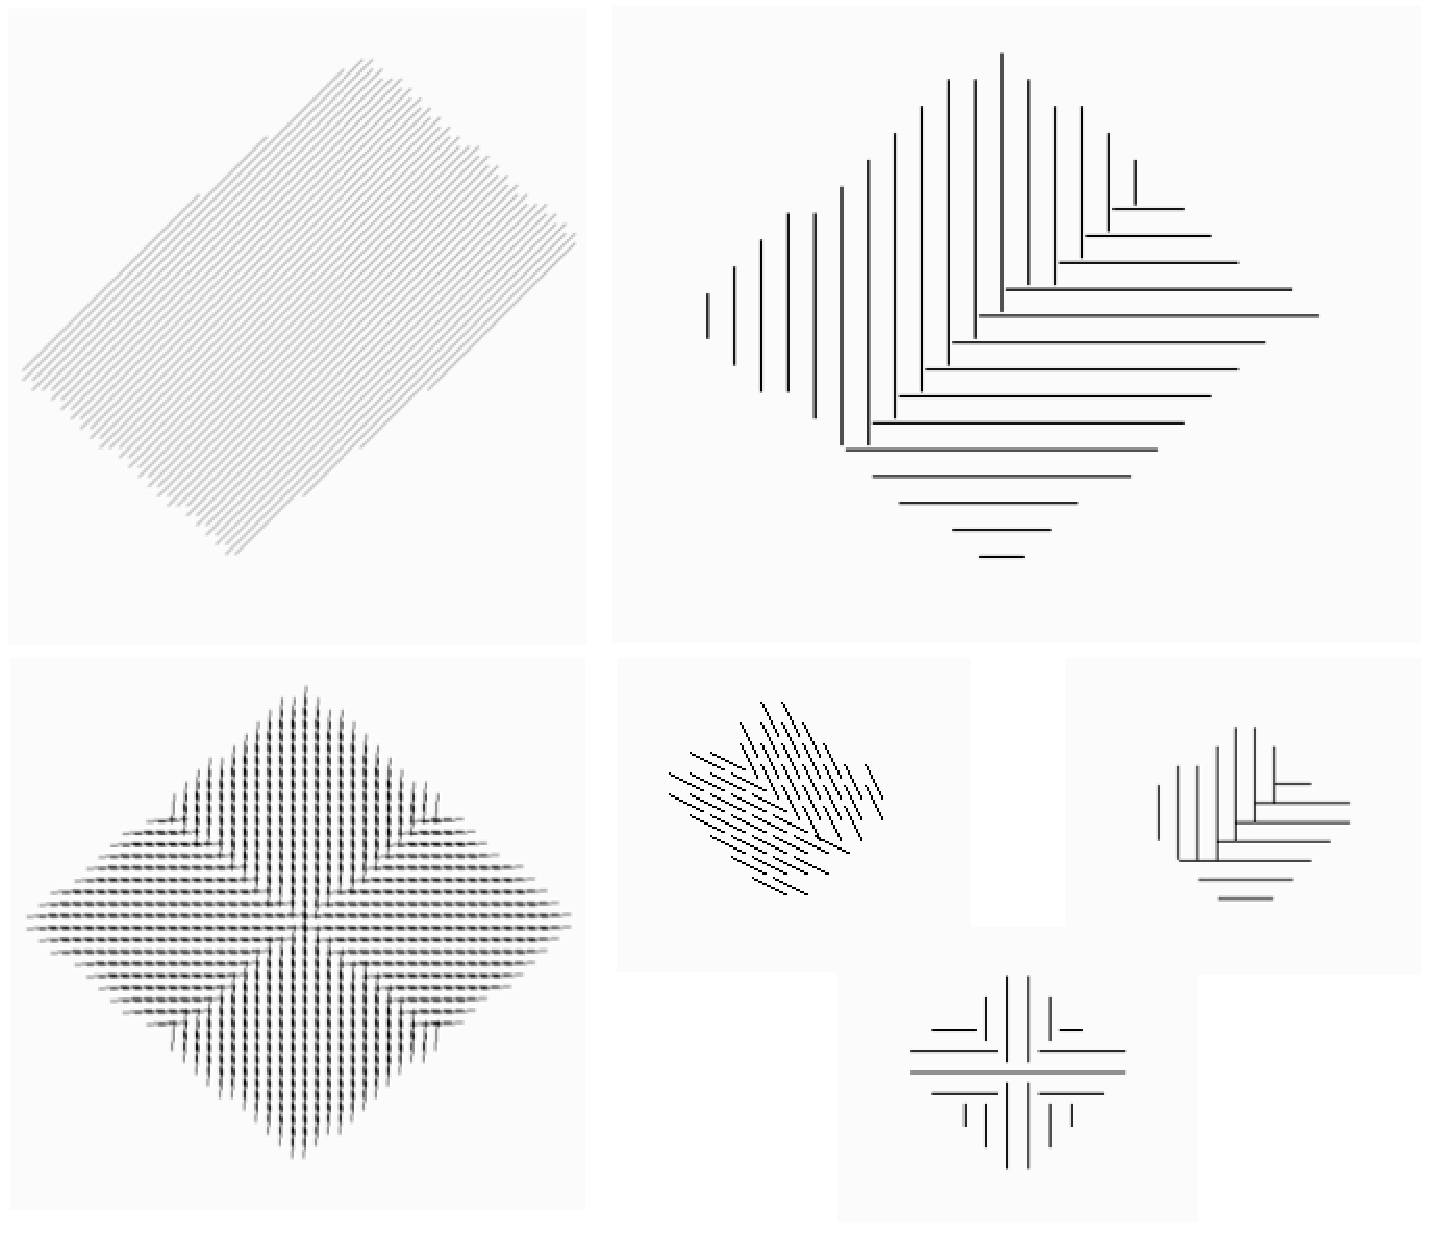
\includegraphics[width=\textwidth]{fig_modphase_back.pdf}
 }
 }
\caption{Examples of MP-multiscale coefficients backprojection.}
\label{fig_modphase_back}
\end{figure*}
Let us provide some essential notation~: we assume that the entries of the phase map $P$ lie in a manifold $\mathcal{M}$ 
(\textit{e.g.} $\mathcal{M}\equiv S^1$). According to \cite{rahman05}, take $p_0,p_1 \in \mathcal{M}$ and define $Log_{p_0}(p_1)$ 
as the log-map of $p_1$ onto the tangent space $\mathcal{T}_{p_0}$ of $\mathcal{M}$ at $p_0$. The back-projection is obtained 
using the inverse of the log-map $Exp_{p_0}$. \footnote{In differential geometry, the Exp map and Log map are generalizations of 
the usual exponential and logarithm function. Here the manifold $\mathcal{M}$ is a Riemannian manifold. In that case, the Exp map 
at point $p_0$, $Exp_{p_0}(s)$ is the map which takes a vector $s$ of the tangent space of $\mathcal{M}$ at $p_0$ and provides the 
point $p_1$ by travelling along the geodesic starting at $p_0$ in the direction s.}\\
For instance, if we choose $\mathcal{M} \equiv S^1$ then $p_0 = \exp(i \theta_0)$ and $p_1 = \exp(i \theta_1)$. The $Exp_{p_0}$ and 
$Log_{p_0}$ maps are then defined as follows~:
\begin{eqnarray}
\forall p_1 \in S^, \,\,\,  Log_{p_0} (p_1) & = & \theta_1 - \theta_0 \\
\forall s \in \mathbb{R} \,\,\, Exp_{p_0} (s) & = & exp(i(\theta_0 + s))
\end{eqnarray}
The multiscale transform for manifold valued data introduced in \cite{rahman05} is equivalent to a two-step interpolation-refinement 
scheme similar to the lifting scheme described in~\cite{wave:sweldens98}. The wavelet coefficients and low pass approximation pixels 
are then computed as follows at each scale $j$ and pixel $k$~:
\begin{eqnarray}\label{eq:mani}
w_{j+1,k}^P & = & Log_{c_{j,2k+1}^P}\left(\mathcal{P}(c_{j,2k}^P)\right)   \\
c_{j+1,k}^P & = & Exp_{c_{j,2k}^P} ( -\mathcal{U}(w_{j+1,k}^P))
\label{eq:mani2}
\end{eqnarray}
The wavelet coefficient $w_{j+1,k}^P$ at pixel $k$ and scale $j$ is the projection of its prediction/interpolation $\mathcal{P}(c_{j,2k}^P)$ 
onto the tangent space $\mathcal{T}_{c_{j,2k+1}^P}$ of $\mathcal{M}$ at $c_{j,2k+1}^P$. The low pass approximation $c_{j+1,k}^P$ at scale $j+1$ 
is computed by updating $c_{j,2k}^P$ from the wavelet coefficient $w_{j+1,k}^P$.\\
The main advantage of this scheme is its ability to capture local regularities while guaranteeing the low pass approximation to belong to 
the manifold $\mathcal{M}$. Indeed, the wavelet coefficient $w_{j+1,k}^P$ at pixel $k$ and scale $j+1$ is computed as the $Exp$ map at 
$c_{j,2k+1}^P$ of an approximation $\mathcal{P}(c_{j,2k}^P)$ of $c_{j,2k}^P$.\\
Note also that even if the definitions of the $Exp_{p_0}$ and $Log_{p_0}$ maps involve the absolute phase $\theta(k)$ (\textit{i.e.} $tan(\theta(k)) = U_k/Q_k$), 
at least they only require the computation of differences of phases values thus avoiding the explicit manipulation of an absolute phase.\\
However the non-linearity of the proposed transform is a major drawback when considering denoising and restoration applications.\\ 

\paragraph{Illustration~:\\}
In the case of polarized data, the entries of the phase map $P$ lie in $\mathcal{M} \equiv S^1$. In the following experiments, $\mathcal{P}$ and $\mathcal{U}$ are chosen such that~:
\begin{eqnarray}
w_{j+1}^P & = & Log_{c_{j,2k+1}^P}(c_{j,2k}^P)  \\
c_{j+1,k}^P & = & Exp_{c_{j,2k}^P} \left( - \frac{w_{j+1}^P}{2}\right)
\end{eqnarray}
This multiscale transform is invertible and its inverse is computed as follows~:
\begin{eqnarray}
c_{j,2k}^P & = & Exp_{c_{j+1,k}^P} \left(\frac{w_{j+1}^P}{2}\right)\\
c_{j,2k+1}^P & = & Exp_{c_{j,2k}^P}\left( w_{j+1}^P \right)   
\end{eqnarray}
The picture in Figure~\ref{fig_modphase_back} features some examples of backprojections of MP-multiscale coefficients.

\subsection{Undecimated MP-multiscale transform}
For image restoration purposes, the use of undecimated multiscale transforms has been shown to provide better results than decimated transforms~\cite{starck:book98,starck:book06}. 
The aforementioned modulus/phase multiscale analysis can be extended to an undecimated scheme consisting in~: i) applying an undecimated wavelet transform to the modulus map, 
ii) analyzing the phase map P using an extension to the undecimated case of the multiscale transform described in \cite{rahman05}. In that case, Equations~\eqref{eq:mani} 
and \eqref{eq:mani2} are replaced with the following equations~:
\begin{eqnarray}\label{eq:maniu}
c_{j+1,k}^P & = & Exp_{c_{j,k}^P} ( \mathcal{F}(c_{j,.}^P))\\
w_{j+1}^P & = & Log_{c_{j+1,k}^P}\left(c_{j,k}^P\right)  
\end{eqnarray}
where $\mathcal{F}(c_{j,.}^P) = \sum_l h_{l} Log_{c_{j,k}}\left(c_{j,k-2^jl}\right)$ with $\sum_l h_l = 1$ and $h_l > 0$. The low pass 
approximation $c_{j+1,k}^P$ is then computed from a linear combination (linear filter) of a neighborhood $\{c_{j,k-2^jl}\}_l$ of $c_{j,k}$ 
weighted by the positive scalars $\{h_l\}_l$. Note that from scale $j$ to scale $j+1$, the spatial size of the neighborhood increases 
by a factor $2$ which would be equivalent to downsize by a factor $2$ the band pass filter of the classical wavelet decomposition scheme.\\

\subsection{Example}
In the case of polarized data, the entries of the phase map $P$ lie in $\mathcal{M} \equiv S^1$. In the following experiments, $\mathcal{F}$ is chosen such that~:
\begin{eqnarray}
c_{j+1,k}^P & = & Exp_{c_{j,k}^P}\left(\sum_l h_{l}Log_{c_{j,k}}\left(c_{j,k-2^jl}^P\right)\right)  \\
w_{j+1,k}^P & = & Exp_{c_{j,k}^P} \left(c_{j+1,k}^P\right)
\end{eqnarray}
where~:
\begin{equation}
h_l = \left\{
\begin{array}{ccc}
0 & \mbox{ if } & l < -2 \mbox{ or } l > 2 \\
1/16 &\mbox{ if }& l=-2 \mbox{ or } l=2 \\
1/4 &\mbox{ if }& l=-1 \mbox{ or } l=1\\
3/8 &\mbox{ if }& l= 0
\end{array}
\right.
\end{equation}
This multiscale transform is invertible and its inverse is computed as follows~:
\begin{equation}
 c_{j,k}^P  =  Exp_{c_{j+1,k}^P } \left(- w_{j+1,k}^P\right)  
\end{equation}

\begin{figure*}[htb]
 \vbox{
 \centerline{
 \hbox{
 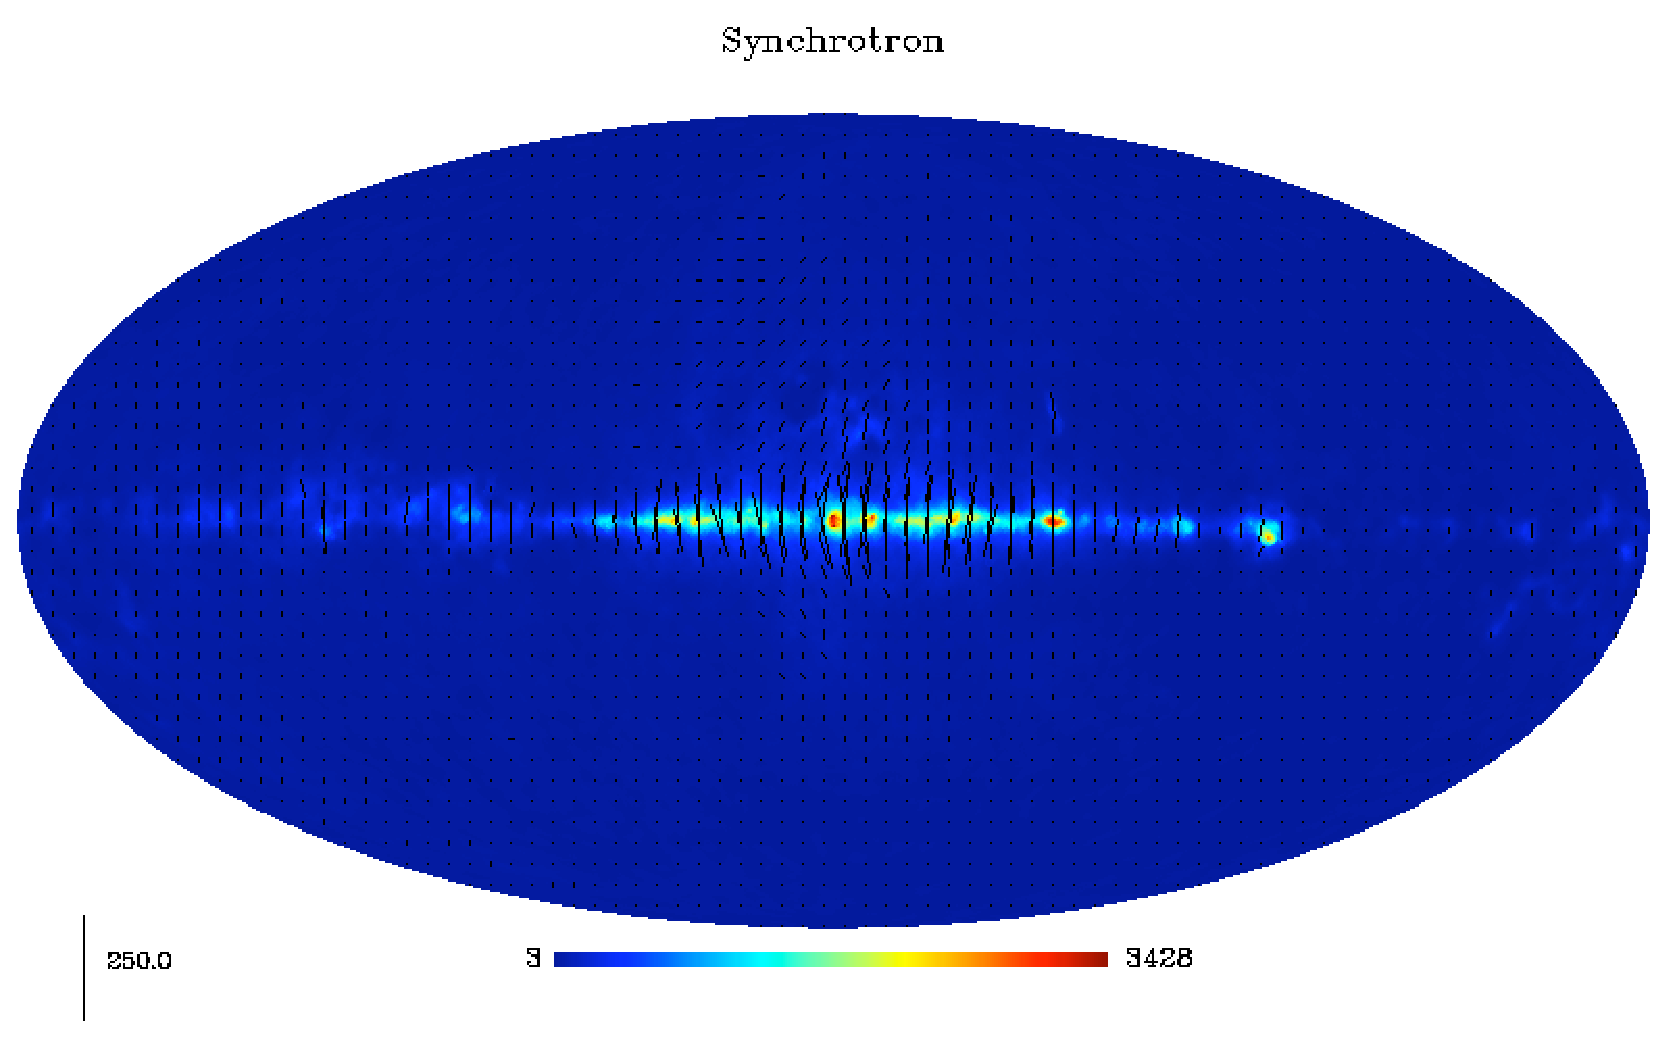
\includegraphics[width=7cm]{fig_mol_synchrotron.pdf}
 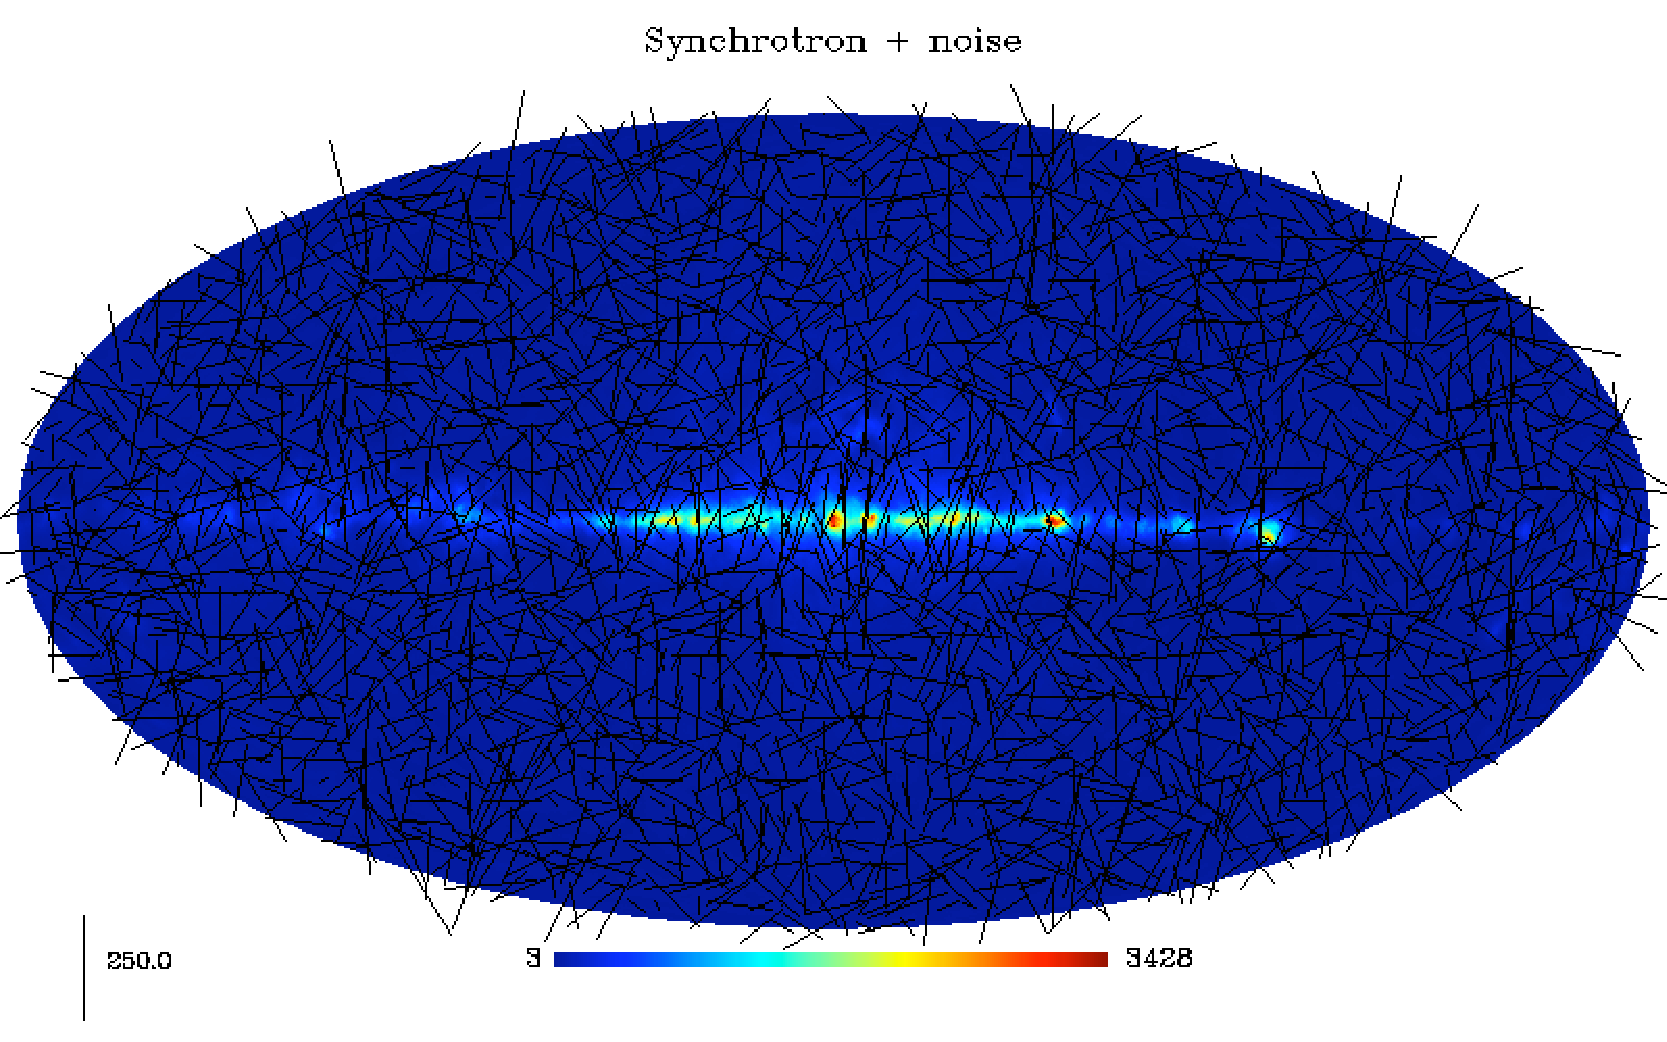
\includegraphics[width=7cm]{fig_mol_synchrotron_noise.pdf}
 }
 }
 \centerline{
 \hbox{
 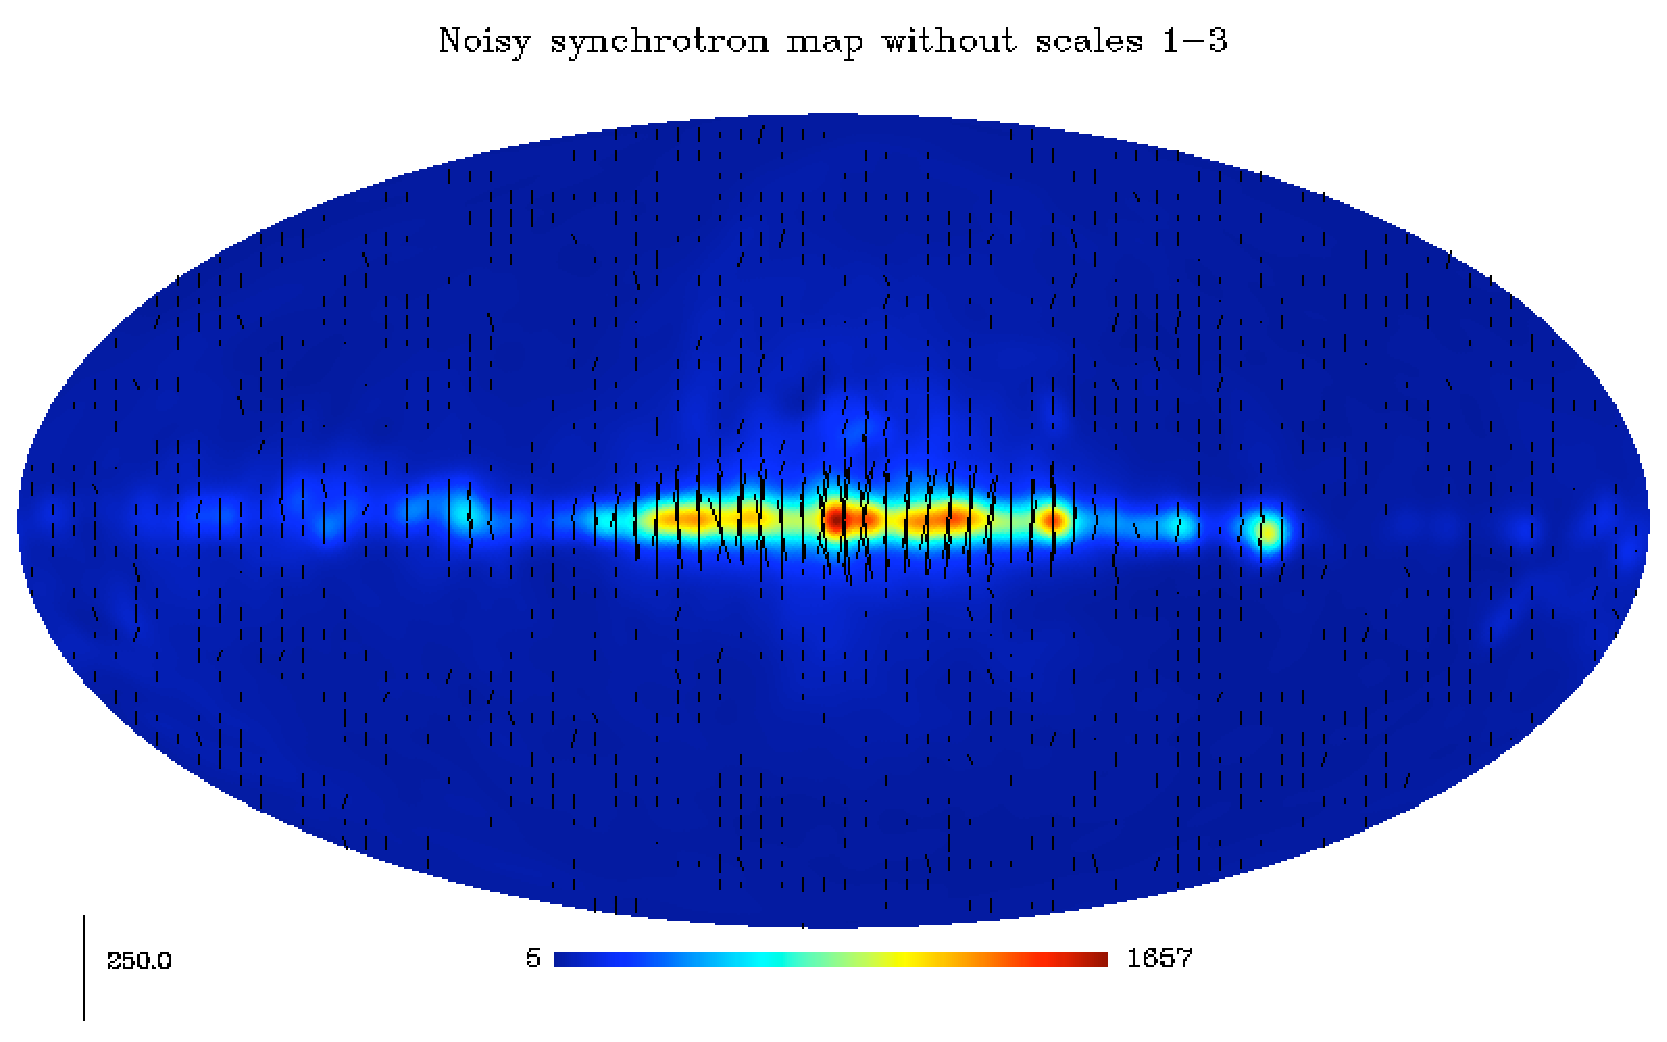
\includegraphics[width=7cm]{fig_mol_synchrotron_noise_no_scale1-3.pdf}
 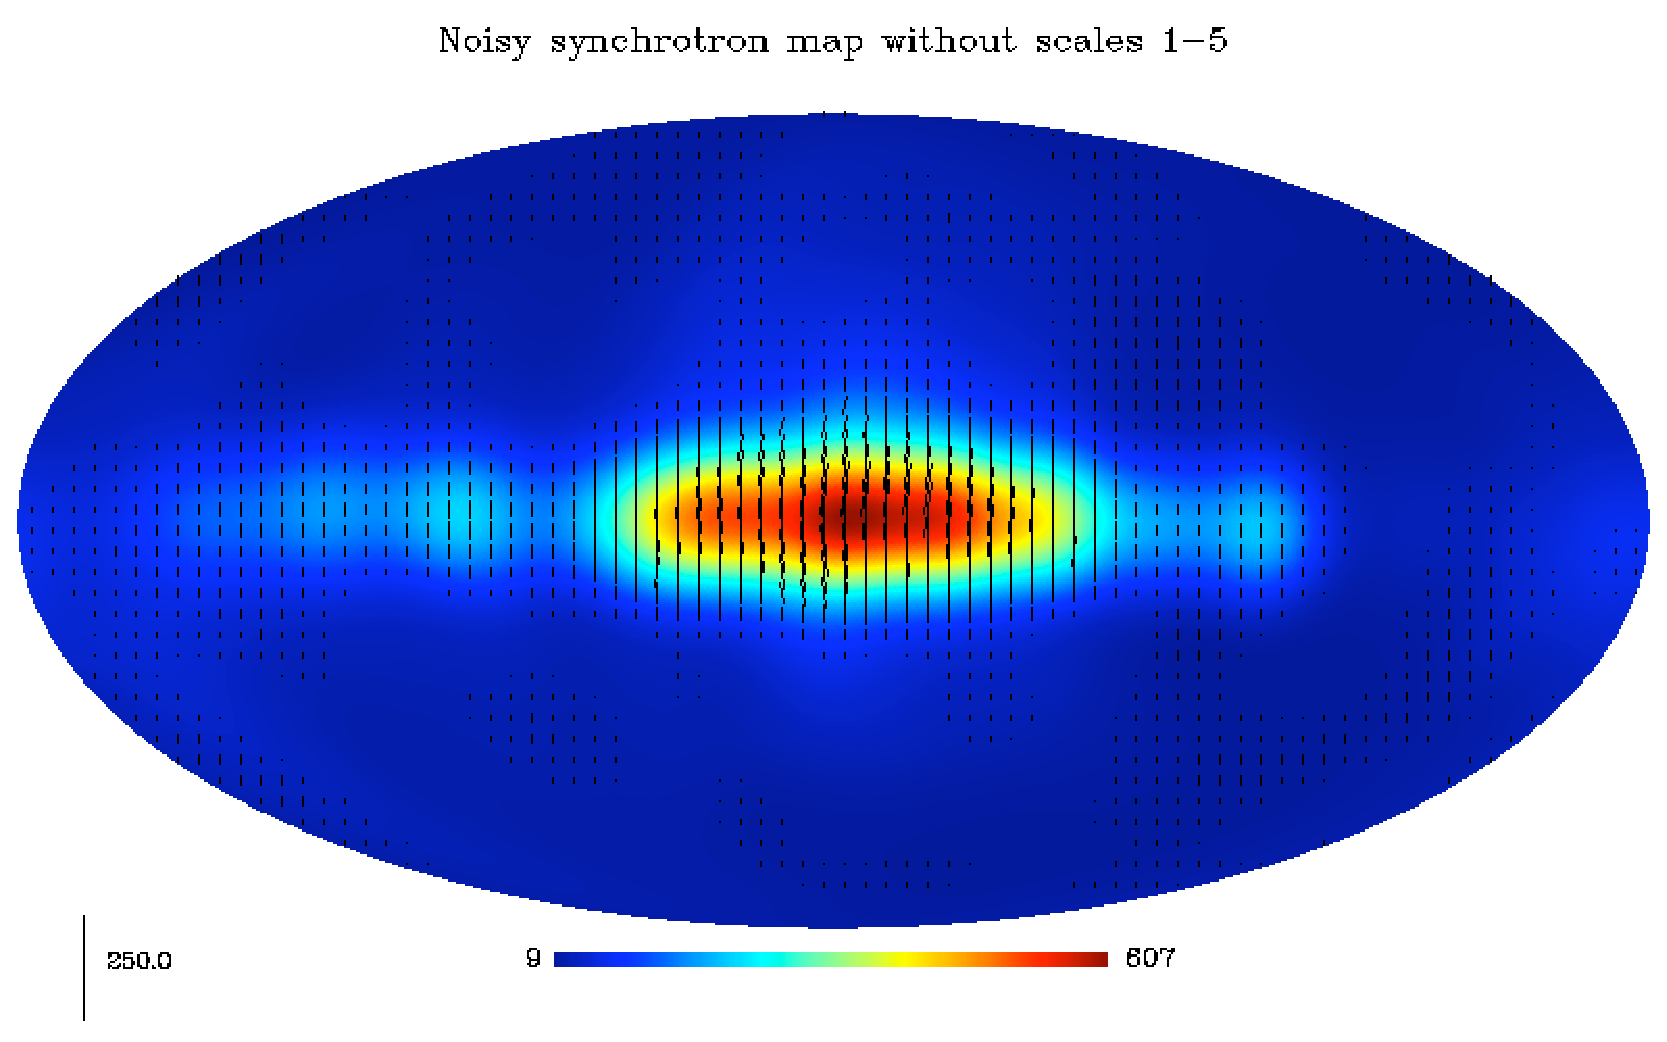
\includegraphics[width=7cm]{fig_mol_synchrotron_noise_no_scale1-5.pdf}
 }
 }
 }
\caption{ Polarized field smoothing - \textit{top left~:} simulated synchroton emission.  \textit{top right~:} same field corrupted by additive noise.
 \textit{bottom left~:} MP-multiscale reconstruction after setting to zero all coefficients from the three first scales.
\textit{bottom right~:} MP-multiscale reconstruction after setting to zero all coefficients from  the five first scales.}
\label{fig_modphase_smoothfield}
\end{figure*}
Fig.~\ref{fig_modphase_smoothfield} top  shows a simulated polarized field of the synchrotron emission and its noisy version.
We have applied the MP-multiscale transform and we remove the first three scales (i.e. we put all coefficients to zero) before 
reconstructing. The resulting image is shown on the bottom left of Fig.~\ref{fig_modphase_smoothfield}. The bottom right of 
Fig.~\ref{fig_modphase_smoothfield} corresponds to the same experiment, but by removing the five first scales. We can see that 
the field is smoother and smoother, but respecting the large scale structure of the field. This transform will be very well suited 
to CMB studies where the phase is analyzed independently of the modulus, such as in~\cite{coles05,naselsky05}.

%---------------------------------------------------------------------------------------------------------------------------------------
%---------------------------------------------------------------------------------------------------------------------------------------


\section{Polarized Wavelet Transform using Spherical Harmonics}
\label{sec:pol_iwt}

\subsection{Isotropic Undecimated Wavelet Transform on the Sphere (UWTS) }
\label{sec:UWTS}

\begin{figure*}[htb]
\centerline{
 \hbox{
 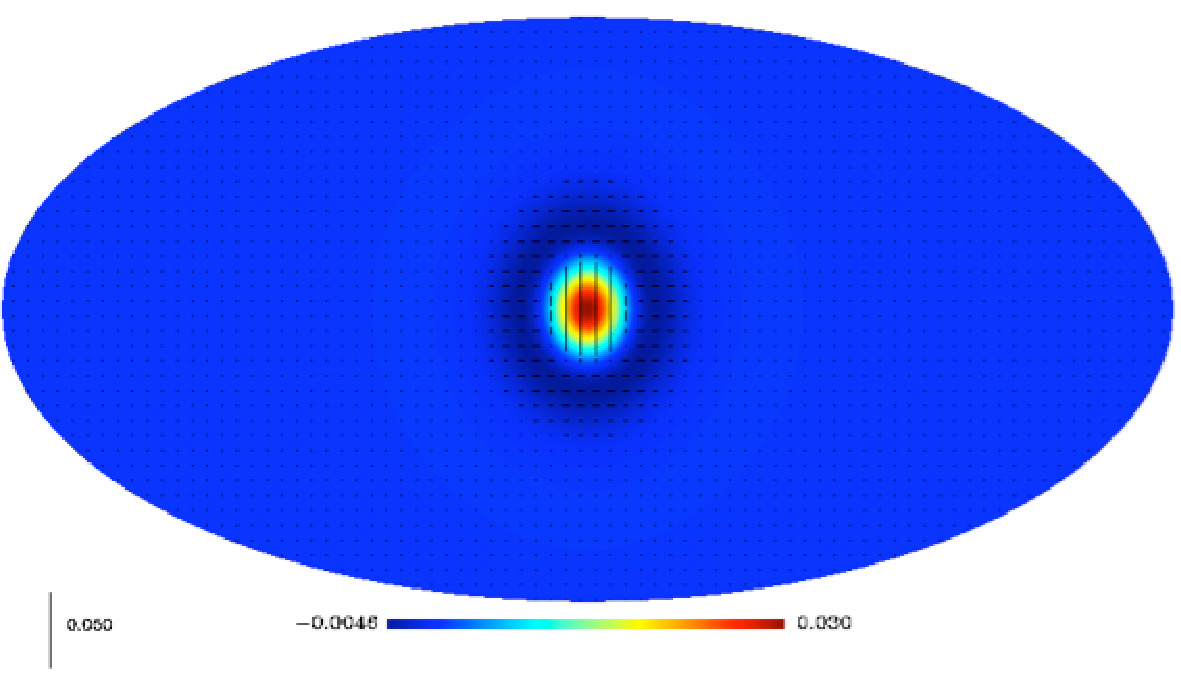
\includegraphics[width=7cm]{fig_q_iwt_back.pdf}
 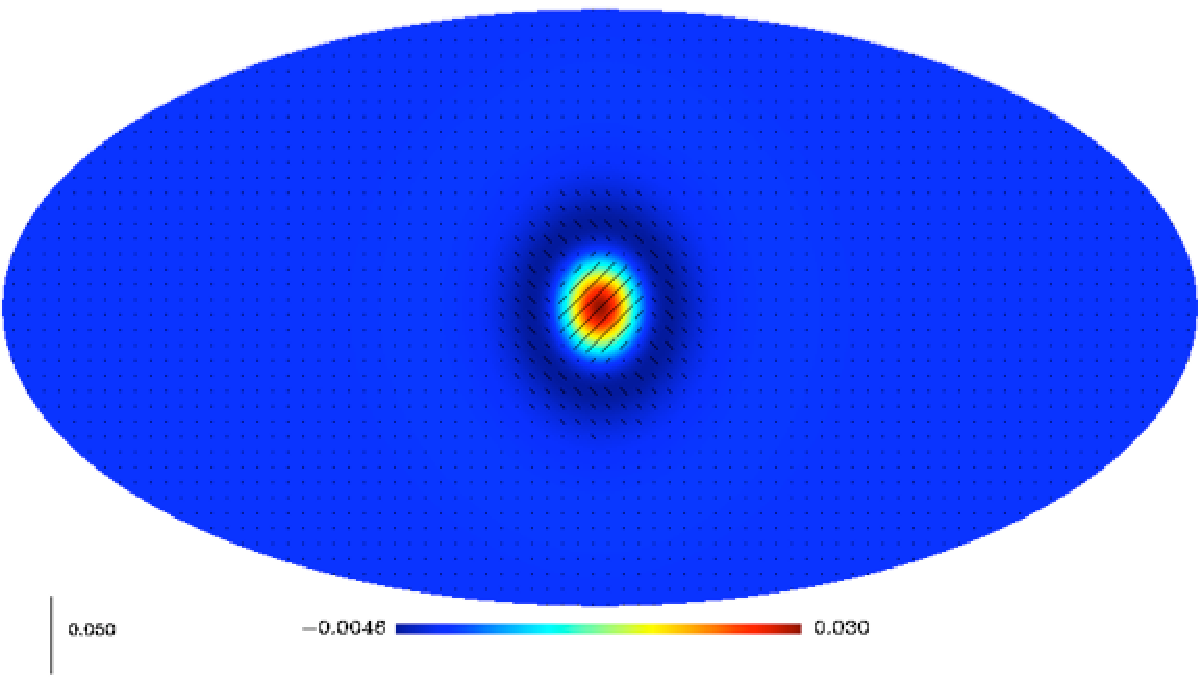
\includegraphics[width=7cm]{fig_u_iwt_back.pdf}
 }
 }
\caption{Q-isotropic wavelet transform backprojection (left) and U-isotropic wavelet backprojection (right).}
\label{fig_qu_iwt_back}
\end{figure*}


%---------------------------------------------------------------------------------------------------------------------------------------
The undecimated isotropic transform on the sphere described in~\cite{starck:sta05_2} is similar in many respects to the usual 
\emph{ \`a trous} isotropic wavelet transform. It is obtained using a zonal scaling function $\phi_{l_c}(\vartheta, \varphi)$ 
which depends only on colatitude $\vartheta$ and is invariant with respect to a change in longitude $\varphi$. It follows that 
the spherical harmonic coefficients $\hat \phi_{l_c} (l,m)$ of $\phi_{l_c}$ vanish when $m \ne 0$ which makes it simple to compute 
those spherical harmonic coefficients $\hat c_{0}(l,m)$ of $c_0 = \phi_{l_c} * f$ where $*$ stands for convolution :
\begin{eqnarray}
 \hat c_{0}(l,m) = \widehat{\phi_{l_c} * f} (l,m) = \sqrt{\frac{4\pi}{2l+1} } \hat \phi_{l_c} (l,0) \hat f(l,m) 
\end{eqnarray}
A possible scaling function~\cite{starck:book98}, defined in the spherical harmonics representation, is $\phi_{l_c}(l, m) = {2 \over 3} B_{3} ( { {2 l} \over {l_{c} } } )$ 
where $B_{3}$ is the cubic B-spline compactly supported over $[-2, 2]$. Denoting $\phi_{2^{-j} l_{c} }$ a rescaled version of 
$\phi_{l_{c}}$ with cut-off frequency $2^{-j} l_{c}$, a multi-resolution decomposition of $f$ on a dyadic scale is obtained recursively : 
\begin{eqnarray}
c_0   & = &  \phi_{ l_{c} }  * f    \nonumber    \\
c_j    &=&   \phi_{2^{-j}  l_{c}  }  * f  =   c_{j-1} * h_{j-1} \nonumber    \\
\end{eqnarray}
where the zonal low pass filters $h_{j}$ are defined by 
\begin{eqnarray}
 \hat{H}_{j}(l,m)  & =  &  \sqrt{\frac{4\pi}{2l+1} }  \hat h_{j}(l,m)  \nonumber \\
 &  =  & \left\{
  \begin{array}{ll}
  \frac {   \hat \phi_{\frac{l_{c}}{2^{j+1}} }(l,m)   }   {  \hat  \phi_{  \frac{l_{c}}{2^{j}} }(l,m)   } & \mbox{if }  l  < \frac{ l_{c}} {2^{j+1}} \quad \textrm{and}\quad m = 0\\
0 & \mbox{otherwise } \ 
  \end{array}
  \right.
\end{eqnarray}
The cut-off frequency is reduced by a factor of $2$ at each step so that in applications where this is useful such as compression, 
the number of samples could be reduced adequately. Using a pixelization scheme such as Healpix \cite{pixel:healpix}, this can easily 
be done by dividing by 2 the Healpix {\it nside} parameter when computing the inverse spherical harmonics transform. 
% Of course, this is only an approximate \emph{Sampling Theorem} but it proved sufficient for numerical purposes.  However, in the present isotropic undecimated transform, no downsampling is performed  and the maps have the same number of pixels on each scale. Hence the orthogonality requirement is relaxed, which provides us with a higher degree of freedom in the choice and design  of the wavelet function $\psi_{l_c}$ to be used with the scaling function $\phi_{l_c}$. 
As in the \emph{\`a trous} algorithm, the wavelet coefficients can be defined as the difference between two consecutive resolutions, 
$w_{j+1}(\vartheta, \varphi) = c_{j}(\vartheta, \varphi) - c_{j+1}(\vartheta, \varphi)$. This defines a zonal wavelet function $\psi_{l_c}$ as 
\begin{eqnarray}\label{wavelet}
\hat \psi_{\frac{l_c}{2^{j}}}(l,m) = \hat \phi_{\frac{l_c}{2^{j-1}}} (l,m)  - \hat \phi_{\frac{l_c}{2^{j}}}(l,m)
\end{eqnarray}

\begin{figure*}[htb]
\centerline{
\hbox{
 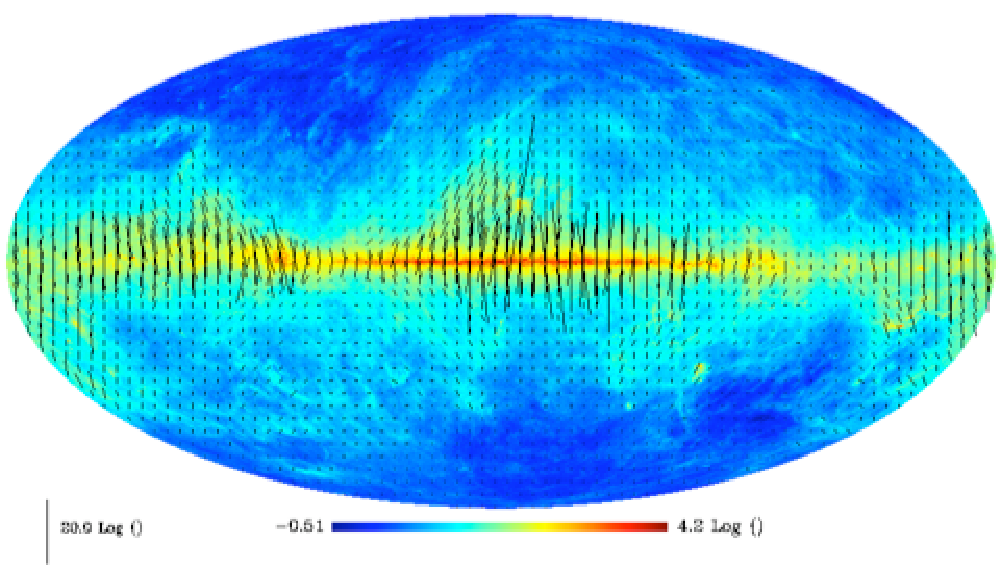
\includegraphics[width=7cm]{fig_dust_input.pdf}
}}
\caption{Simulated observations on the sphere of the polarized galactic dust emission.}
\label{fig_simu_pol_dust}
\end{figure*}

With this particular choice of wavelet function, the decomposition is readily inverted by summing the coefficient maps on all wavelet scales
 \begin{eqnarray}\label{IWT}
   %c_{0}(\vartheta, \varphi) = c_{J}(\vartheta, \varphi) + \sum_{j=1}^{J} w_j(\vartheta, \varphi)
   f(\vartheta, \varphi) = c_{J}(\vartheta, \varphi) + \sum_{j=1}^{J} w_j(\vartheta, \varphi)
\end{eqnarray}
where we have made the simplifying assumption that $f$ is equal to $c_0$. Obviously, other wavelet functions $\psi$ could be used just as well, such as the needlet function~\cite{marinucci08}.

% Also,  because of the redundancy of the described decomposition, the inverse transform  is not unique and in fact this can profitably be used to impose additional constraints on the synthesis functions (\emph{e.g.} smoothness, positivity) used in the reconstruction \cite{starck:sta06}. 

\begin{figure*}[htb]
\centerline{
\vbox{
 \hbox{
 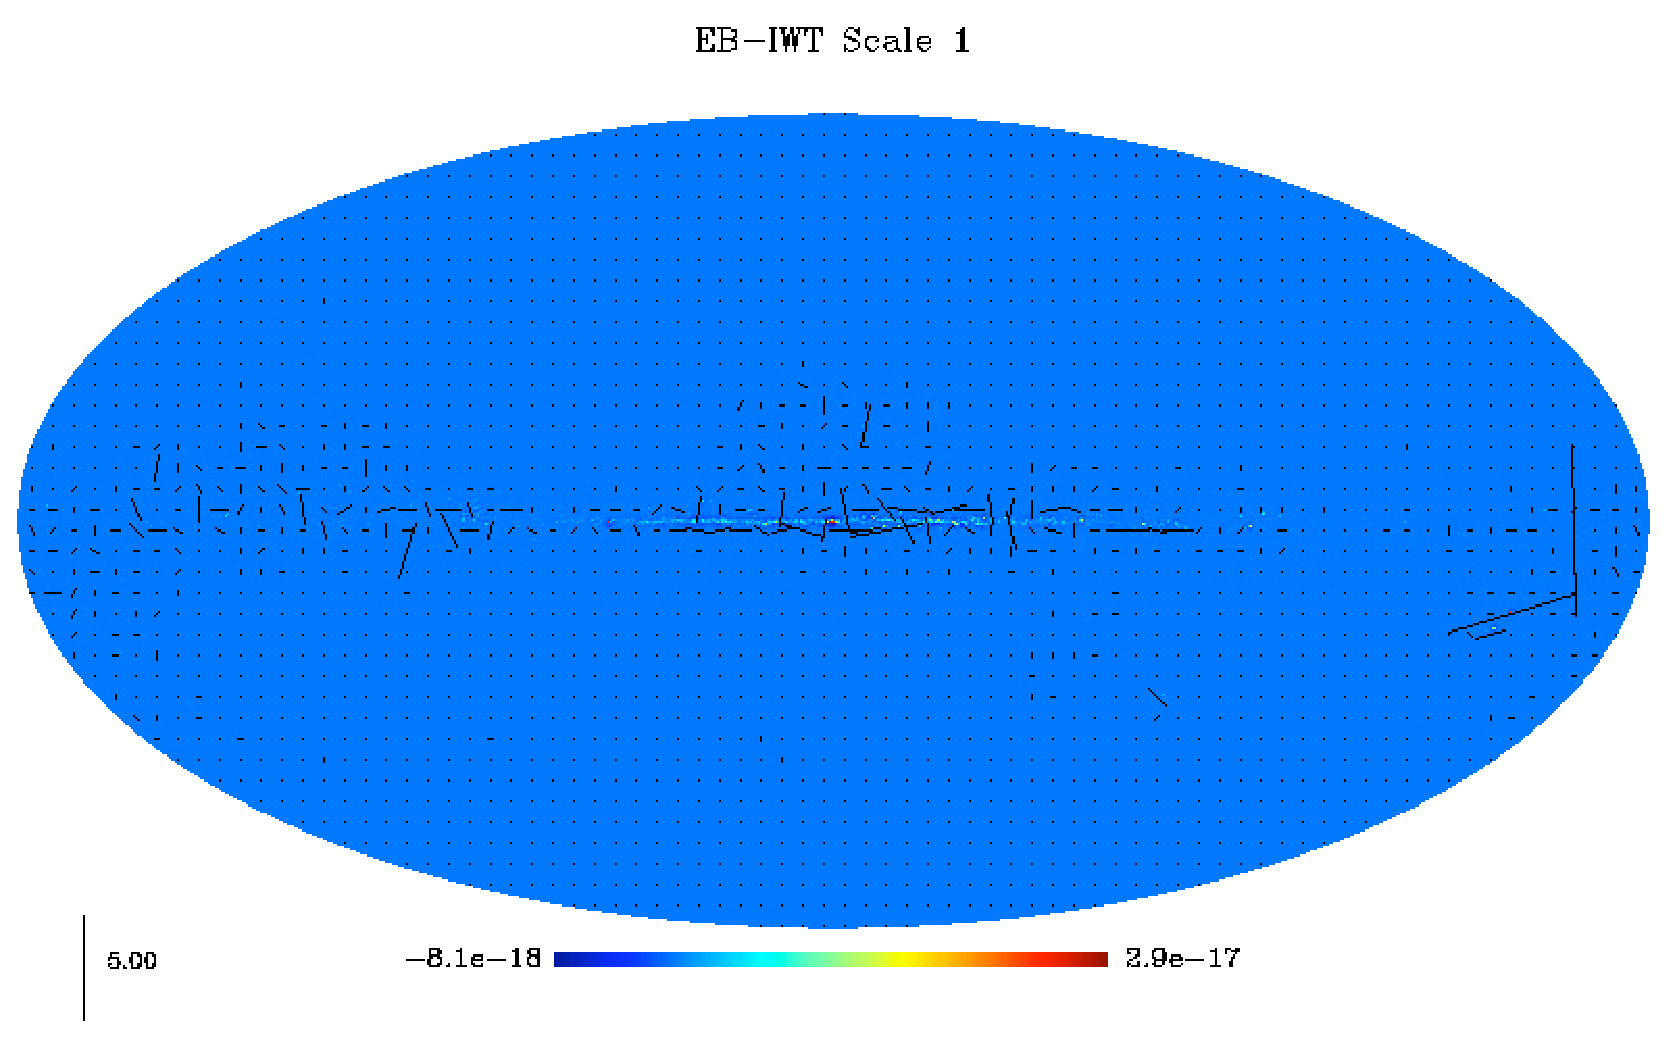
\includegraphics[width=7cm]{fig_ebiwt_scale1.pdf}
 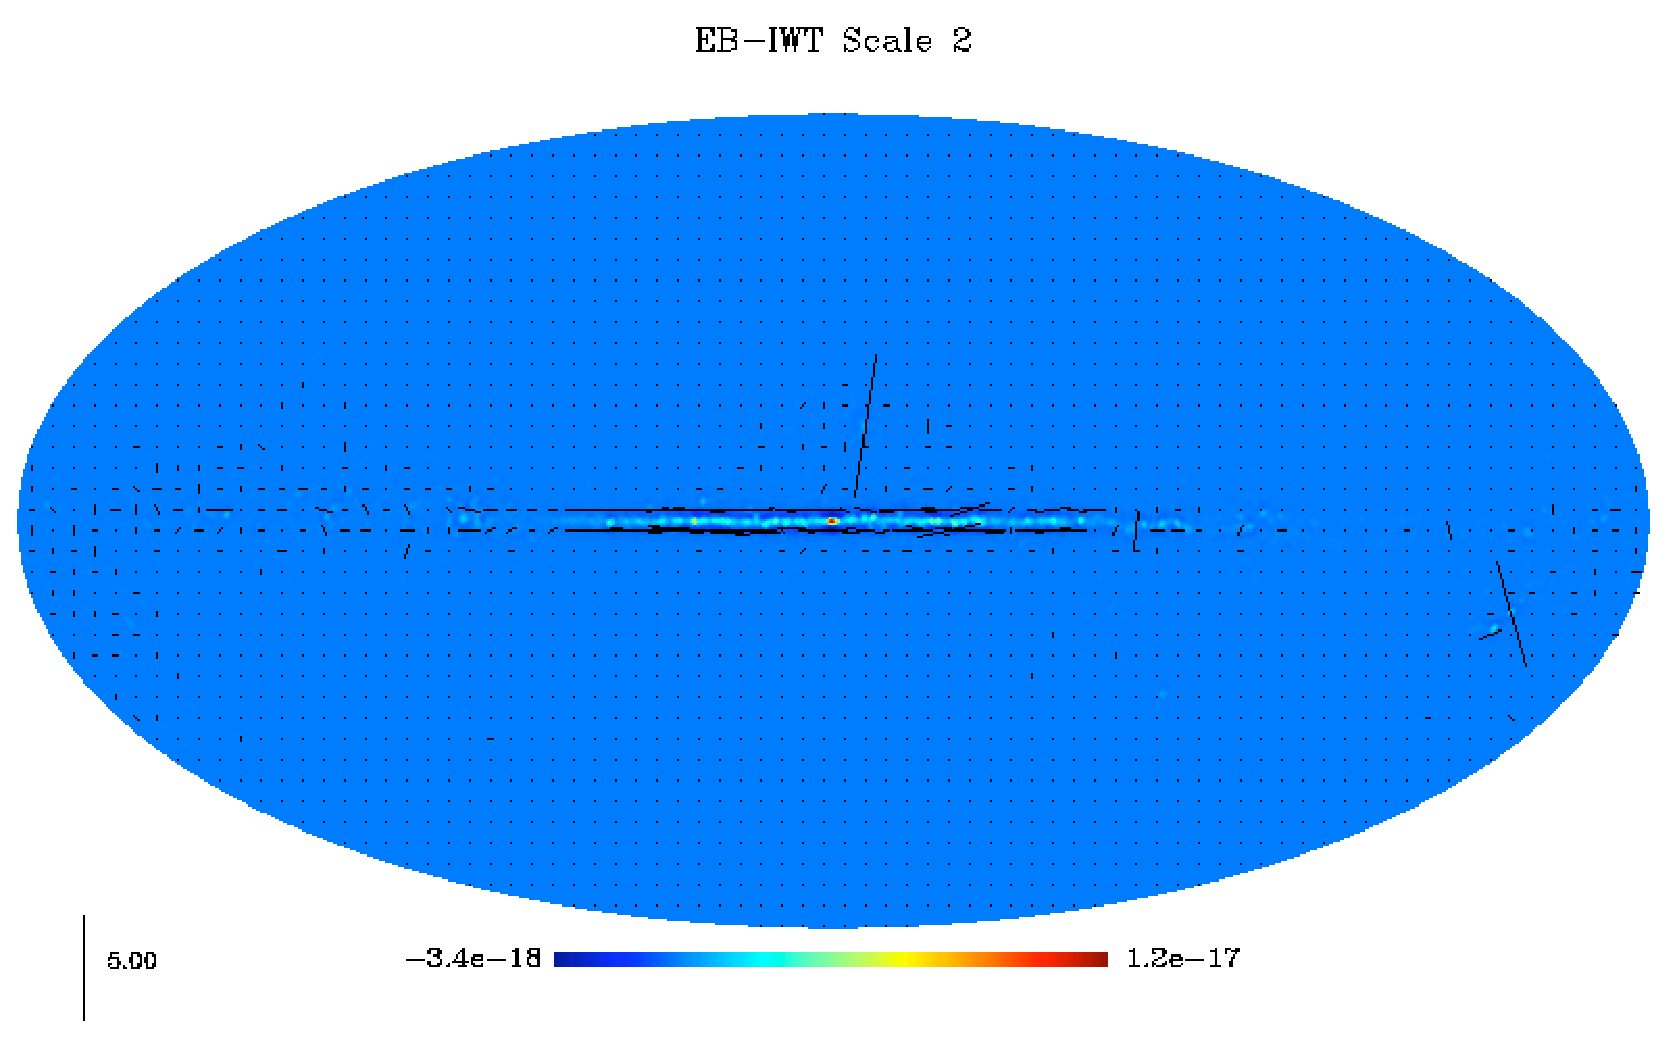
\includegraphics[width=7cm]{fig_ebiwt_scale2.pdf}
 }
 \hbox{
 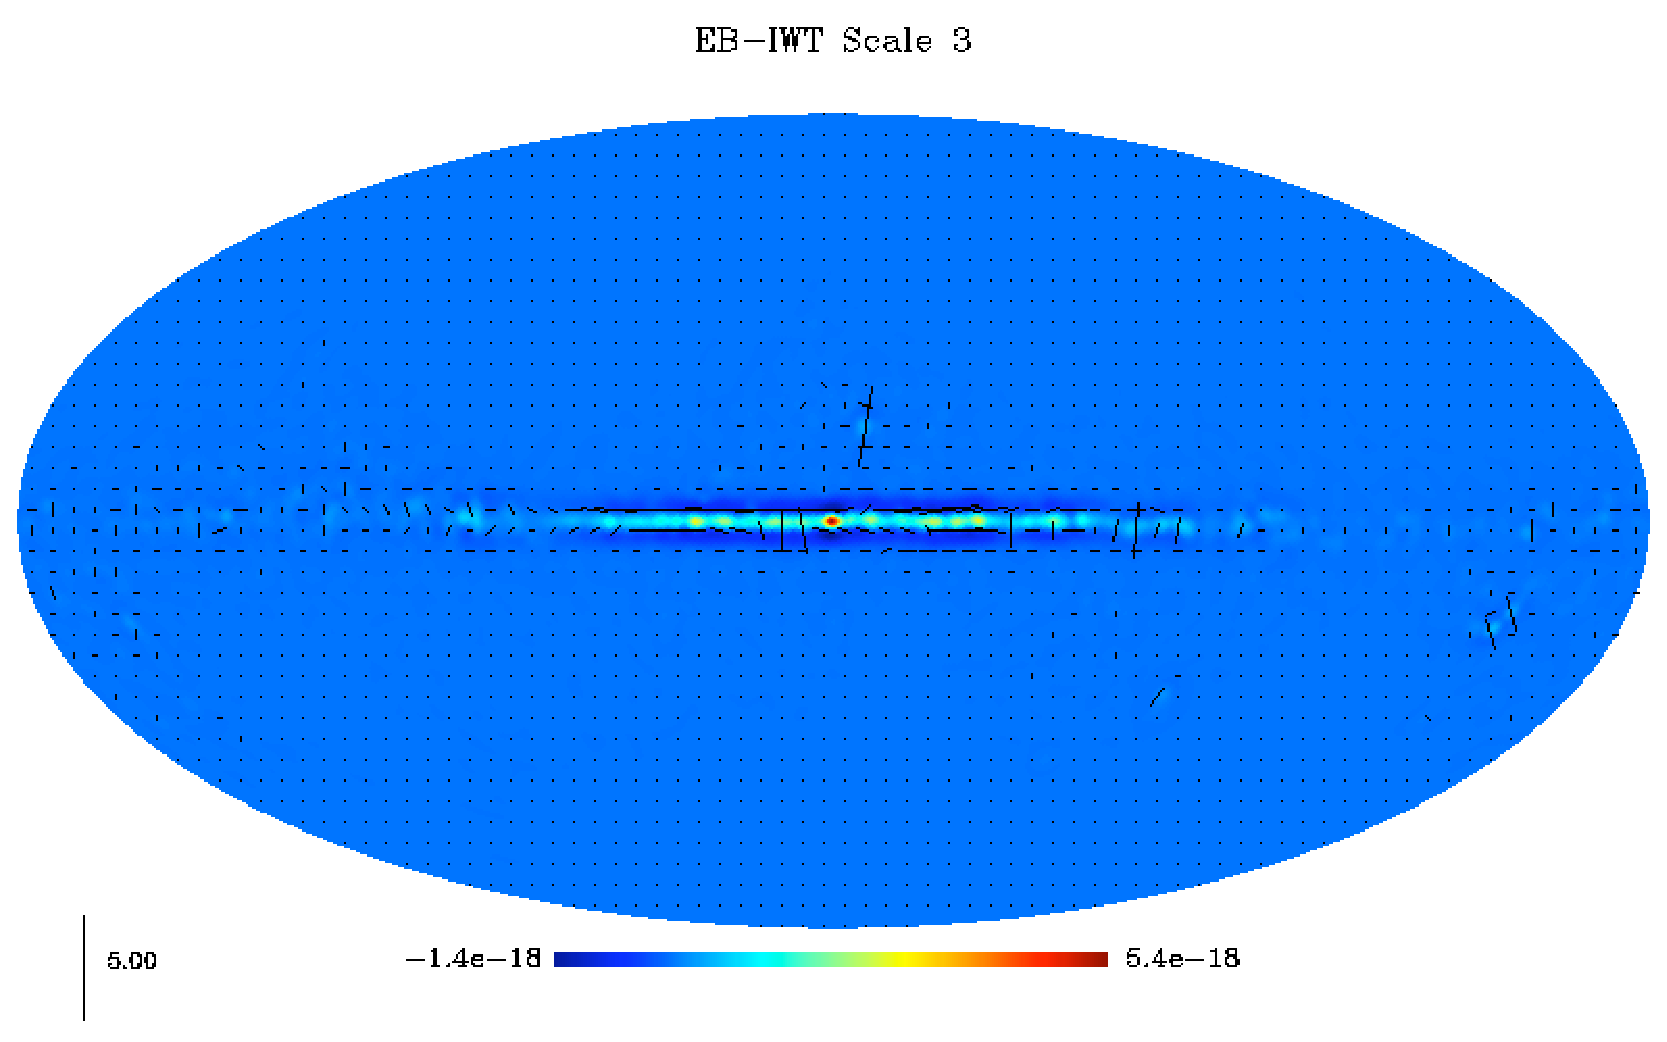
\includegraphics[width=7cm]{fig_ebiwt_scale3.pdf}
 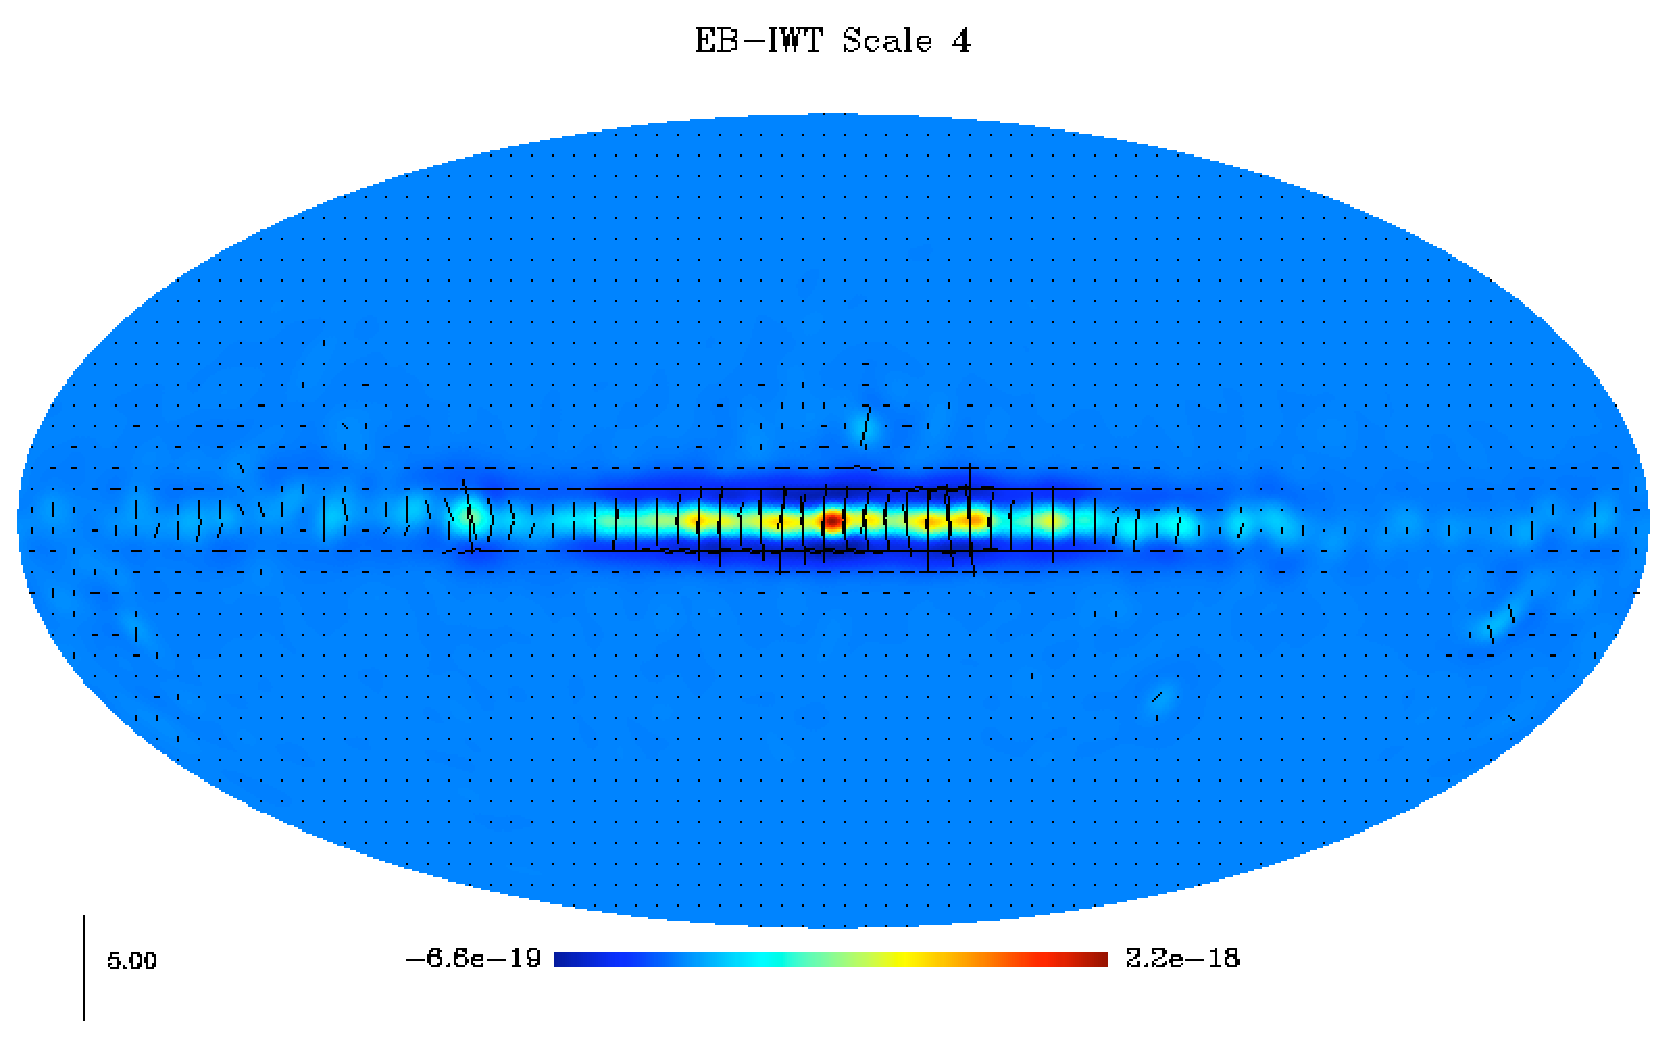
\includegraphics[width=7cm]{fig_ebiwt_scale4.pdf}
 }
  \hbox{
 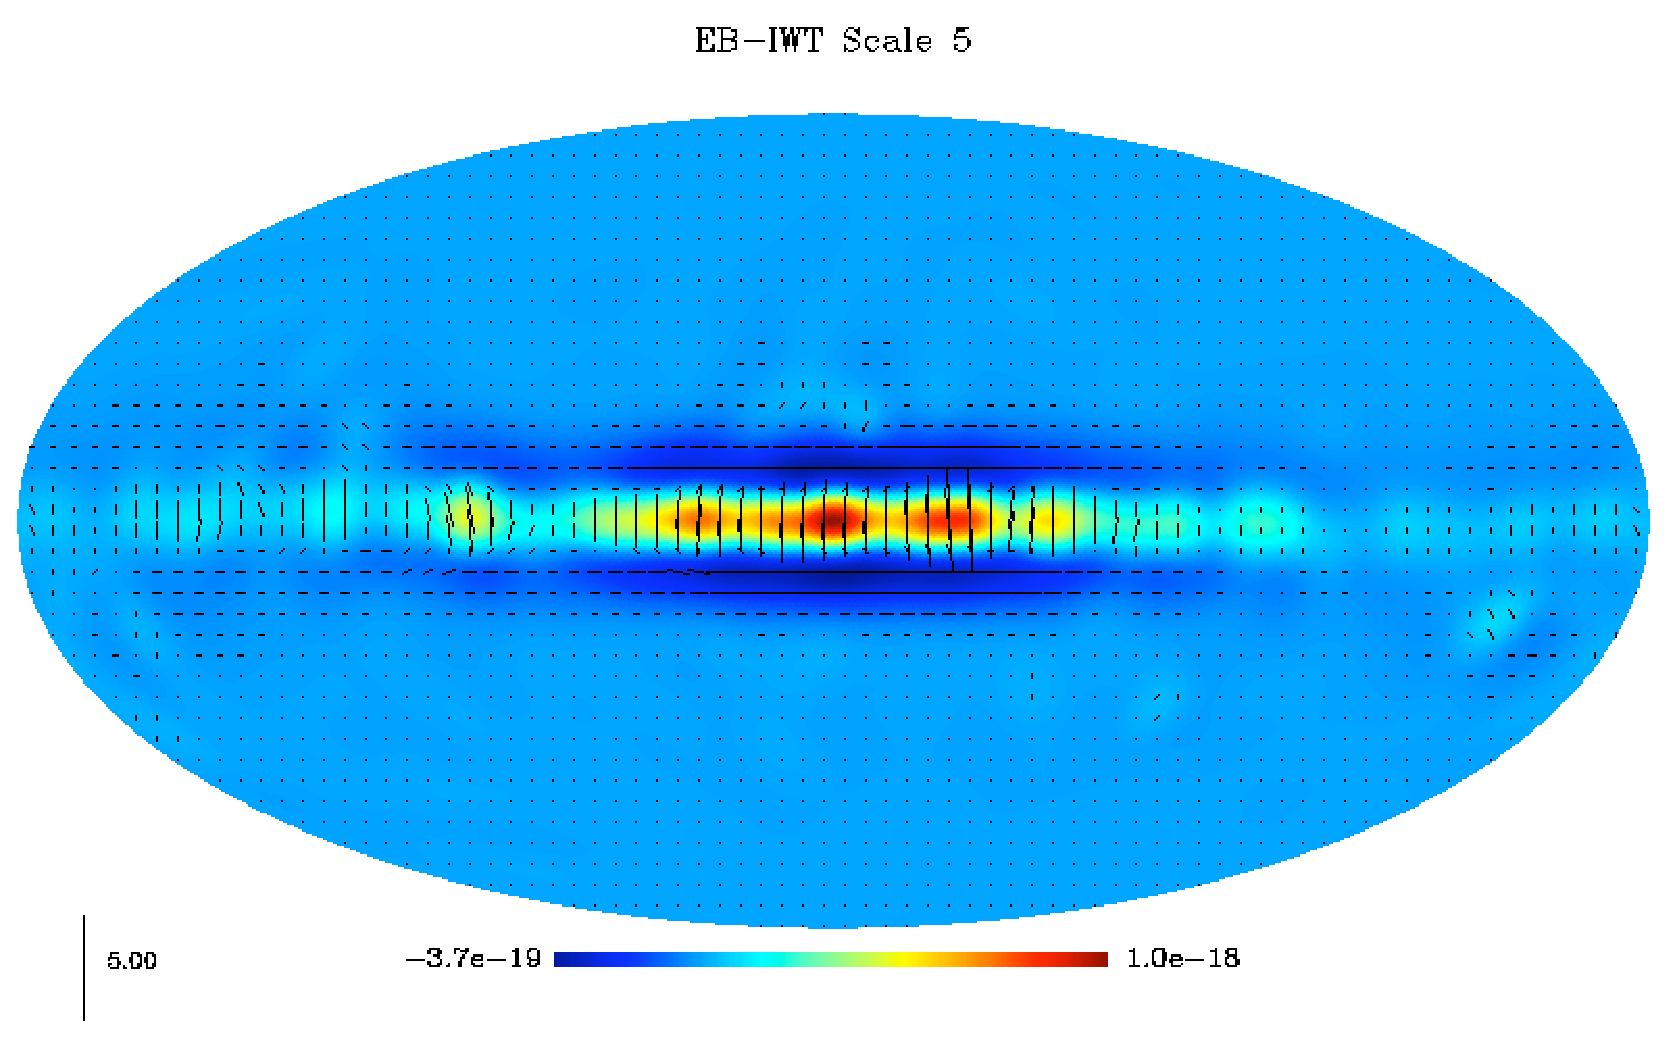
\includegraphics[width=7cm]{fig_ebiwt_scale5.pdf}
 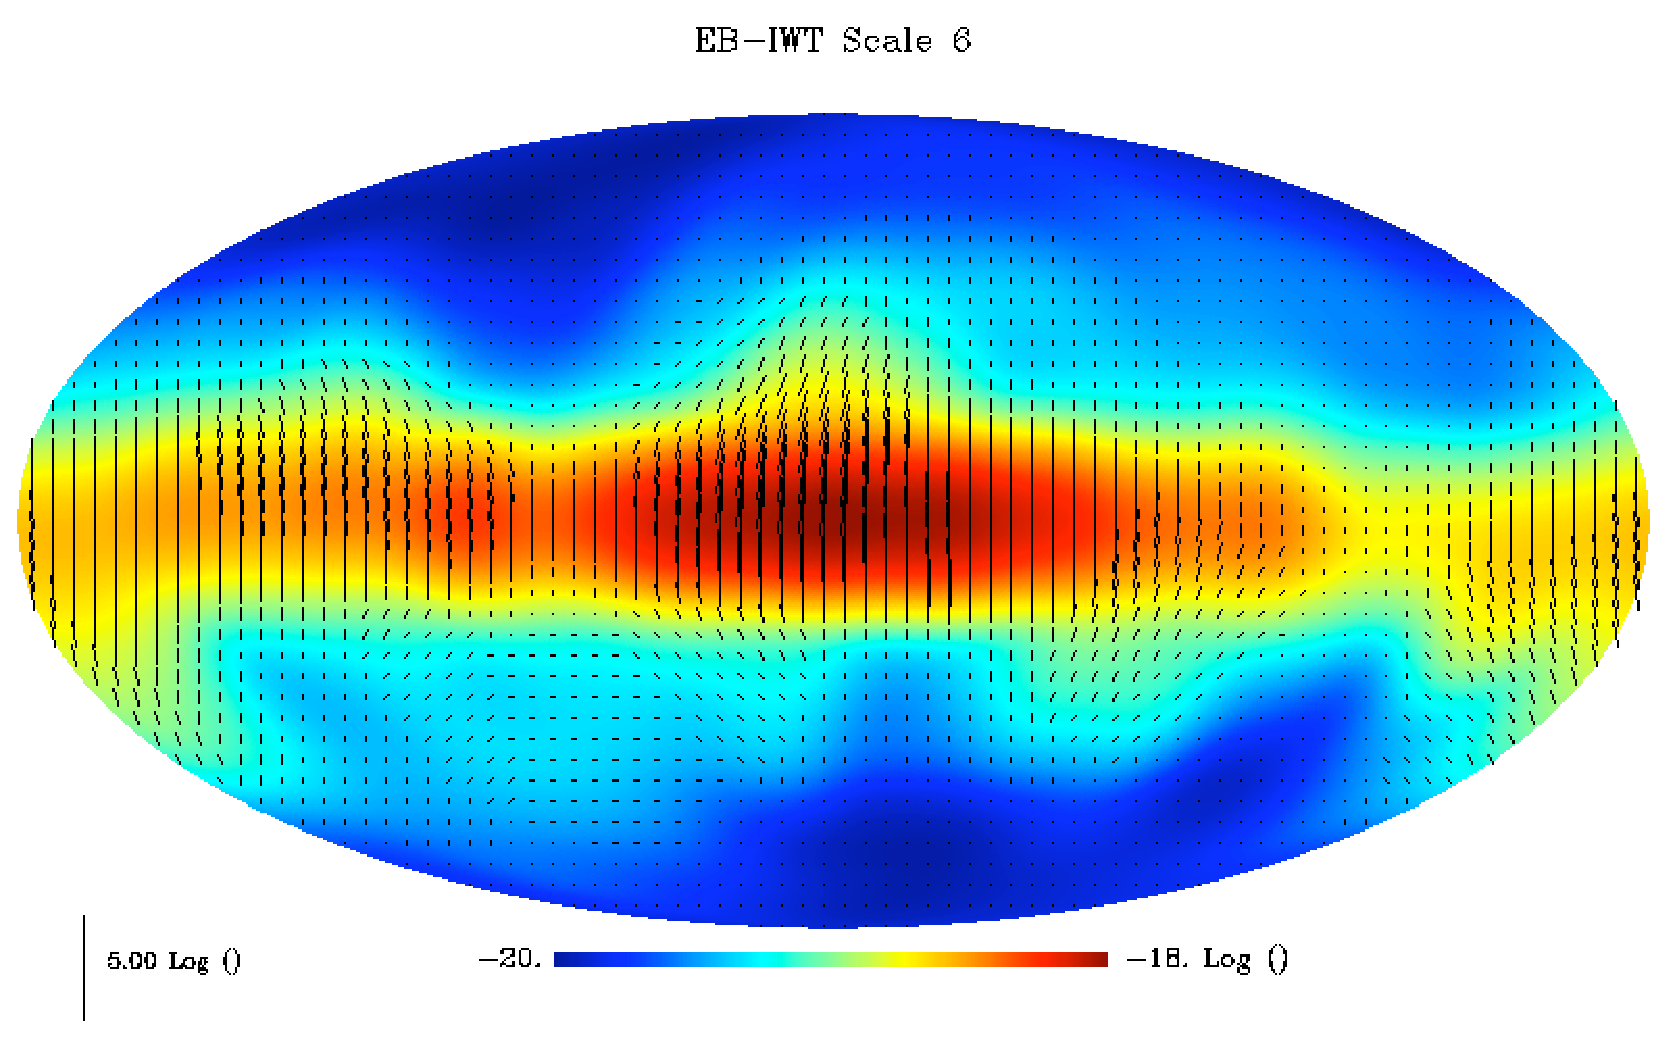
\includegraphics[width=7cm]{fig_ebiwt_scale6.pdf}
 }
  }
 }
\caption{QU-Undecimated Wavelet Transform of the simulated polarized map of galactic dust emission shown in figure~(\ref{fig_simu_pol_dust}).}
\label{fig_quwt_trans_dust}
\end{figure*}

\subsection{Extension to Polarized Data}
By applying the above scalar isotropic wavelet transform to each component $T$, $Q$, $U$ of a polarized map on the sphere, we have~:
\begin{eqnarray}
\label{tqu_iwt}
T(\vartheta, \varphi) & = c_{J}^T (\vartheta, \varphi)+ \sum_{j=1}^{J} w_j^T  (\vartheta, \varphi)\\ \nonumber
Q(\vartheta, \varphi) & = c_{J}^Q (\vartheta, \varphi)+ \sum_{j=1}^{J} w_j^Q (\vartheta, \varphi)\\ \nonumber
U(\vartheta, \varphi) & = c_{J}^U (\vartheta, \varphi)+ \sum_{j=1}^{J} w_j^U (\vartheta, \varphi)
\end{eqnarray}
where $c_{J}^X$ stands for the low resolution approximation to component $X$ and $w_j^X$ is the map of wavelet coefficients of that component on scale $j$. This leads to the following decomposition~:
\begin{eqnarray}
(Q \pm iU)[k] =    (c^Q_{J} \pm c^U_{J,p})[k]   +   \sum_{j=1}^J   ( w_{j}^Q \pm w_{j}^U )[k]
\label{eq_qu_rec_uwt}
\end{eqnarray}
Fig.\ref{fig_qu_iwt_back} shows the backprojection of a Q-wavelet coefficient (left) and a $U$-wavelet coefficient (right).
Fig.~\ref{fig_quwt_trans_dust} shows the undecimated isotropic polarized wavelet transform of the dust image shown on 
Fig.~\ref{fig_simu_pol_dust} using six scales, \textit{i.e.} five wavelet scales and the coarse approximation.
%---------------------------------------------------------------------------------------------------------------------------------------
%---------------------------------------------------------------------------------------------------------------------------------------
\section{Polarized Curvelet Transform}
\label{sec:pol_cur}
% \begin{figure*}
% \centerline{
% \hbox{
% \psfig{figure=fig_back_cur_sphere.ps,bbllx=1cm,bblly=7cm,bburx=20cm,bbury=20cm,height=8.5cm,width=12cm,clip=}
% }}
% \caption{Backprojection of  various curvelet coefficients at different scales and orientations on the sphere.  Each map is obtained by setting all but one of the curvelet coefficients to zero, and applying an inverse curvelet transform. Depending on the scale and the position of the non zero curvelet coefficient, the reconstructed image presents a feature with a given width, length and orientation.}
 %\label{Figure:back_cur}
% \end{figure*}
 \begin{figure*}[htb]
\centerline{
\vbox{
 \hbox{
 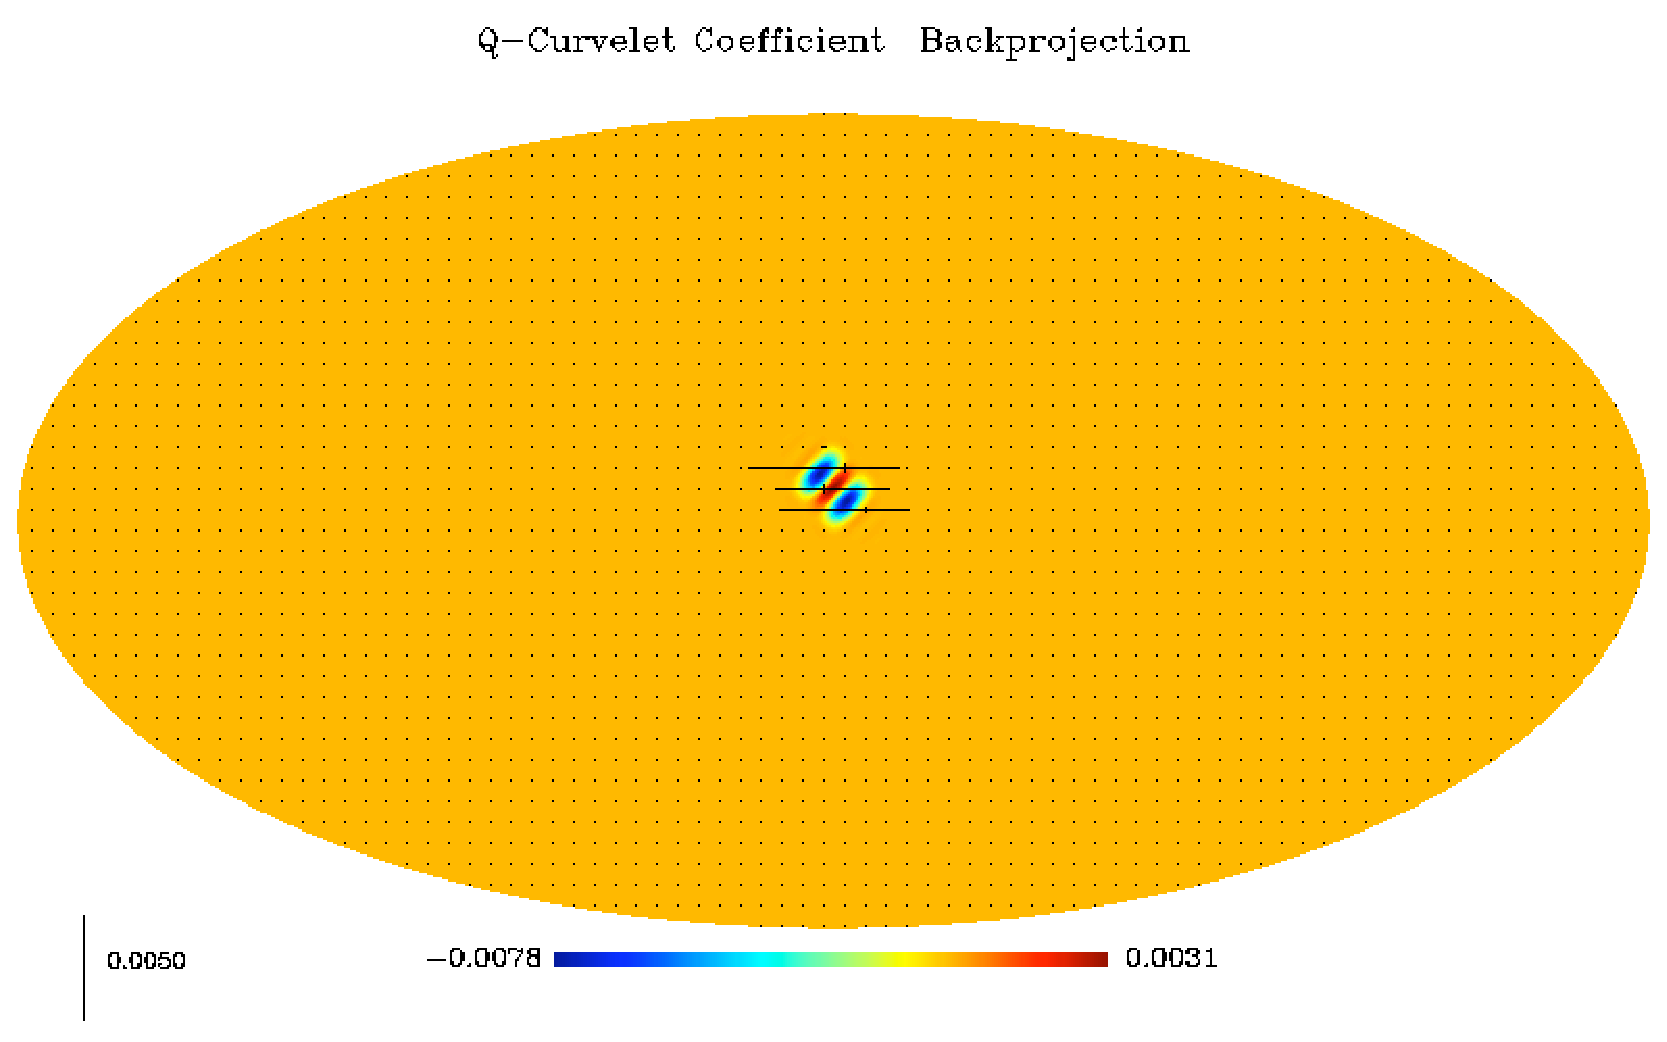
\includegraphics[width=7cm]{fig_mol_backproj_qucur_qj3.pdf}
 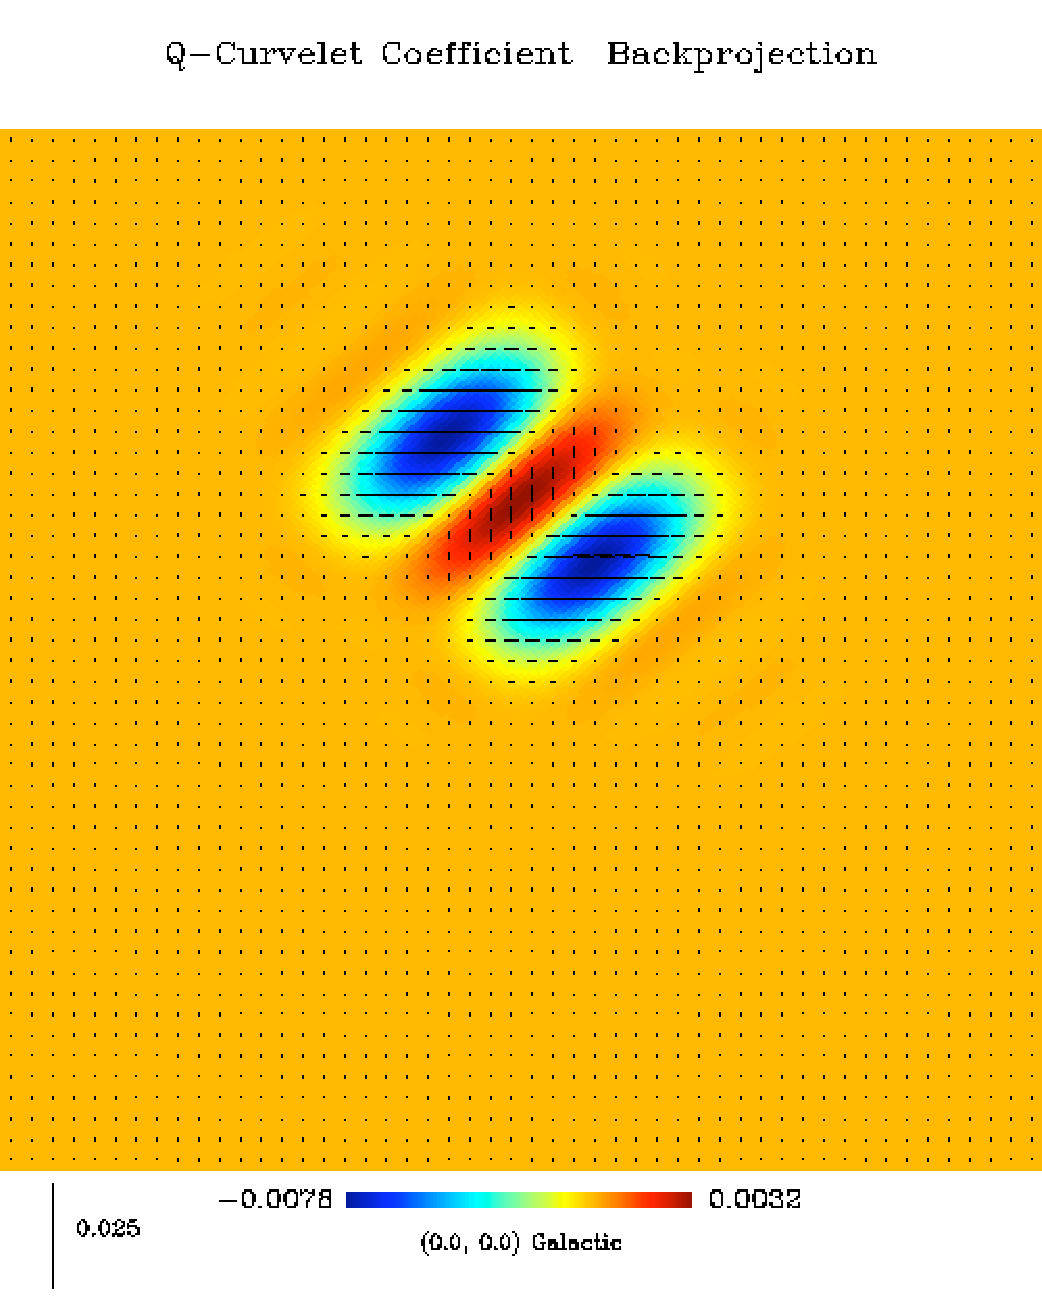
\includegraphics[width=4cm]{fig_backproj_qucur_qj3.pdf}
 }
 \hbox{
 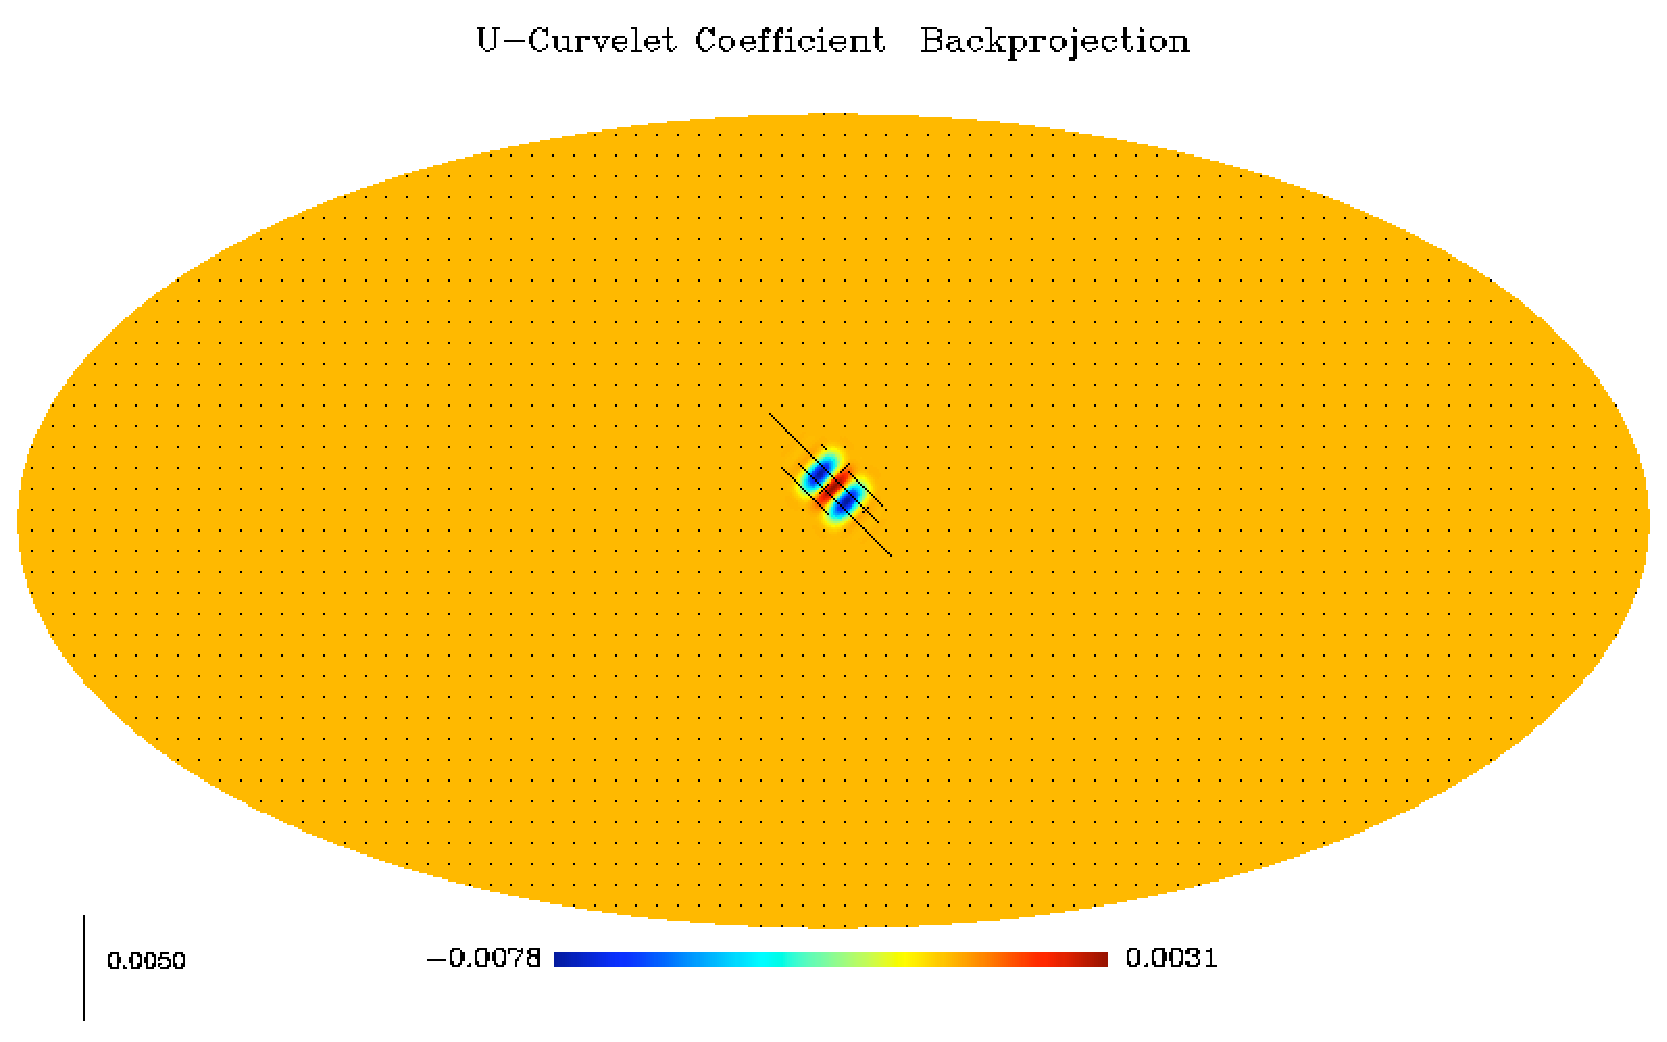
\includegraphics[width=7cm]{fig_mol_backproj_qucur_uj3.pdf}
 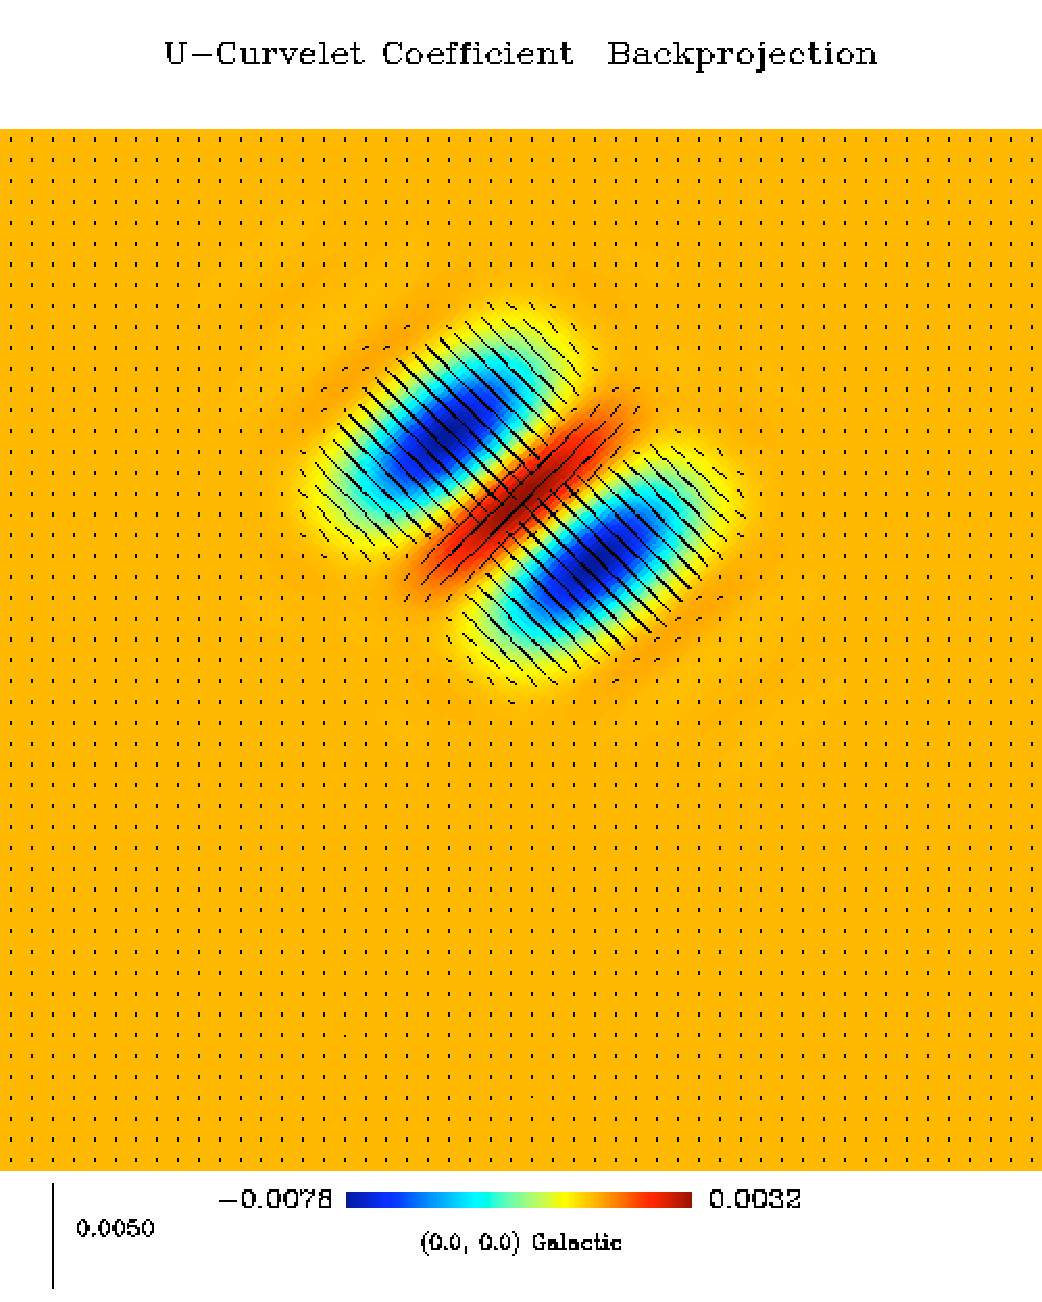
\includegraphics[width=4cm]{fig_backproj_qucur_uj3.pdf}
 }
  }
 }
\caption{Top, Q-curvelet backprojection (left)  and zoom (right). Bottom, U-curvelet backprojection (left)  and zoom. }
\label{fig_qucur_back}
\end{figure*}
The 2D ridgelet transform \cite{cur:candes99_1} was developed in an attempt to overcome some limitations inherent in former multiscale methods 
\emph{e.g.} the 2D wavelet, when handling smooth images with edges \textit{i.e.} singularities along smooth curves. Ridgelets are translation 
invariant \emph{ridge} functions with a wavelet profile in the normal direction. Although ridgelets provide sparse representations of smooth 
images with straight edges, they fail to efficiently handle edges along curved lines. This is the framework for curvelets which were given a 
first mathematical description in \cite{Curvelets-StMalo}. Basically, the curvelet dictionary is a multiscale pyramid of localized directional 
functions with anisotropic support obeying a specific parabolic scaling such that at scale $2^{-j}$, its length is $2^{-j/2}$ and its width is $2^{-j}$. 
This is motivated by the parabolic scaling property of smooth curves. Other properties of the curvelet transform as well as decisive optimality results 
in approximation theory are reported in \cite{Curvelets-StMalo,CandesDonohoCurvelets}. Notably, curvelets provide optimally sparse representations 
of manifolds which are smooth away from edge singularities along smooth curves. Several digital curvelet transforms \cite{cur:donoho99,starck:sta01_3,cur:demanet06} 
have been proposed which attempt to preserve the essential properties of the continuous curvelet transform and many papers \cite{starck:sta04,felix2008,starck:sta04} 
report on their successful application in image processing experiments. The so-called first generation discrete curvelet described in \cite{cur:donoho99,starck:sta01_3} 
consists in applying the ridgelet transform to sub-images of a wavelet decomposition of the original image. By construction, the sub-images are 
well localized in space and frequency and the subsequent ridgelet transform provides the necessary directional sensitivity. This latter implementation 
in combination with the good geometric properties of the Healpix pixelization scheme, inspired the digital curvelet transform on the sphere~\cite{starck:sta05_2}. 
The digital curvelet transform on the sphere is clearly invertible in the sense that each step of the overall transform is itself invertible. 
The curvelet transform on the sphere has a redundancy factor of $16J + 1$ when $J$ scales are used, which may be a problem for handling huge data sets 
such as from the future Planck-Surveyor experiment. This can be reduced by substituting the pyramidal wavelet transform to the undecimated wavelet 
transform in the above algorithm. More details on the wavelet, ridgelet, curvelet algorithms on the sphere can be found in \cite{starck:sta05_2}. 
As for the isotropic wavelet on the sphere, a straightforward extension to polarized data will consist in applying successively the curvelet transform 
on the sphere to the three components $T$, $Q$ and $U$. Figure~\ref{fig_qucur_back} shows the backprojection of a Q-curvelet coefficient and 
U-curvelet coefficient. Clearly, the shapes of these polarized curvelet functions are very different from the polarized wavelet functions.%---------------------------------------------------------------------------------------------------------------------------------------
%---------------------------------------------------------------------------------------------------------------------------------------
\section{Polarized E/B Wavelet and E/B Curvelet}
\label{sec:pol_eb}

\subsection{Introduction}
We have seen that the generalization of the Fourier representation for polarized data on the sphere is the spin-2 spherical harmonics basis denoted $_{\pm 2}Y_{\ell m}$: 
\begin{equation} 
Q \pm i U  = \sum_{\ell, m}  { _{\pm 2}a_{\ell m}}   {_{\pm 2}Y_{\ell m} }
\end{equation} 
  
At this point, it is convenient~\cite{zalda} to introduce the two quantities denoted $E$ and $B$ which are defined on the sphere by 
\begin{eqnarray}\label{EB}
E = &  \sum_{\ell, m}   a_{\ell m} ^E Y_{\ell m} =  \sum_{\ell, m}  - \frac{ 1}{2}   ({_{ 2}a_{\ell m}}  +  {_{- 2}a_{\ell m}} )    Y_{\ell m} \\ \nonumber
B = & \sum_{\ell, m}   a_{\ell m} ^B Y_{\ell m} =  \sum_{\ell, m}  i \frac{ 1}{2}    ({_{ 2}a_{\ell m}}  -  {_{- 2}a_{\ell m}} )   Y_{\ell m} 
\end{eqnarray} 
%\begin{equation}\label{EB}
%E =  \sum_{\ell, m}   a_{\ell m} ^E Y_{\ell m} =  \sum_{\ell, m}  - \frac{   {_{ 2}a_{\ell m}}  +  {_{- 2}a_{\ell m}}  }  {2}  Y_{\ell m}  \quad \quad 
%B =  \sum_{\ell, m}   a_{\ell m} ^B Y_{\ell m} =  \sum_{\ell, m}  i \frac{   {_{ 2}a_{\ell m}}  -  {_{- 2}a_{\ell m}}  }  {2}   Y_{\ell m} 
%\end{equation} 
where $Y_{\ell m}$ stands for the usual spin 0 spherical harmonics basis functions. The quantities $E$ and $B$ are derived by applying 
the spin lowering operator twice to $Q + i U$  and the spin raising operator twice to $Q - i U$ so that $E$ and $B$ are real scalar 
fields on the sphere, invariant through rotations of the local reference frame. The normalization of $a_{\ell m} ^E$ and $a_{\ell m} ^B$ 
chosen in the latter definition is purely conventional but it appears to be rather popular~\cite{1997PhRvD..55.1830Z,2003PhRvD..67b3501B}. 
Still, we could multiply $a_{\ell m} ^E$ and $a_{\ell m} ^B$ by some $A_{\ell}$ and we would have just as good a representation of the initial 
polarization maps. Through a change of parity $E$ will remain invariant whereas the sign of pseudo-scalar $B$ will change. The $E$ and $B$ 
modes defined here are not so different from the \emph{gradient} (\emph{i.e. curl} free) and \emph{curl} (\emph{i.e. divergence} free) components 
encountered in the analysis of vector fields. Finally, the spatial anisotropies of the Gaussian CMB temperature and polarization fields are 
completely characterized in this new linear representation by the power spectra and cross spectra of $T$, $E$ and $B$. Thanks to the different 
parities of $T$ and $E$ on one side and $B$ on the other, the sufficient statistics reduce to only four spectra namely $C_\ell^{EE}, C_\ell^{TE}, 
C_\ell^{TT}, C_\ell^{BB}$. For a given cosmological model, it is possible to give a theoretical prediction of these spectra. Aiming at inverting 
the model and inferring the cosmological parameters, an important goal of CMB temperature and polarization data analysis is then to estimate the 
latter power spectra, based on sampled, noisy sometimes incomplete $T$, $Q$ and $U$ spherical maps.  

\subsection{E/B Isotropic Wavelet}
Following the above idea of representing CMB polarization maps by means of $E$ and $B$ modes, we propose a formal extension of the previous 
undecimated isotropic wavelet transform that will allow us to handle linear polarization data maps $T$, $Q$ and $U$ on the sphere. Practically, 
the maps we consider are pixelized using for instance the Healpix pixelization scheme. In fact, we are not concerned at this point with the 
recovery of E and B modes from pixelized or incomplete data maps which itself is not a trivial task. The extension of the wavelet transform 
on the sphere we describe here makes use of the $E$ and $B$ representation of polarized maps described above in a formal way. Given polarization 
data maps $T$, $Q$ and $U$, the proposed wavelet transform algorithm consists of the following steps : 
\vspace{.1cm}
\begin{center}
\begin{minipage}[b]{0.85\linewidth}
\footnotesize{
\begin{enumerate}
\item Apply the spin $\pm 2$ spherical harmonics transform to $Q+iU$ and $Q-iU$. Practically, the Healpix software package provides an implementation 
of this transform for maps that use this pixelization scheme. Otherwise, a fast implementation was recently proposed by \cite{wiauxspin2}.
\item Combine the decomposition coefficients ${ _{2}a_{\ell m}}$ and ${ _{-2}a_{\ell m}}$ from the first step into $a_{\ell m}^E$ and $a_{\ell m}^B$ 
and build \emph{formal} $E$ and $B$ maps associated with $Q$ and $U$ by applying the usual inverse spherical harmonics transform, as in equation~\ref{EB}. 
For numerical and algorithmic purposes, it may be efficient to stay with the spherical harmonics representation of $E$ and $B$.
\item Apply the undecimated isotropic transform on the sphere described above to map $T$ and to the $E$, $B$ representation of the polarization maps. 
\end{enumerate}}
\end{minipage}
\end{center}
\vspace{.1cm}
The wavelet coefficient maps  $w_j^T$, $w_j^E$, $w_j^B$ and the low resolution approximation maps $c_J^T$, $c_J^E$, $c_J^B$ are obtained by applying 
the isotropic undecimated wavelet transform described in section~\ref{sec:UWTS} to the $T$, $E$, $B$ representation of the polarized data. Figure~\ref{fig:UWTSpol} 
shows the result of applying the proposed transform to the polarized CMB data map \emph{ka} \footnote{available at http://lambda.gsfc.nasa.gov/product/map/current/ } 
from the WMAP experiment. The top two images show the initial $Q$ and $U$ maps while the subsequent maps are the low pass and wavelet coefficients'maps 
in a four scale decomposition. The scaling function we used is a cubic box spline as proposed in section~\ref{sec:UWTS}. The wavelet coefficients were 
obtained as the difference between two successive low pass approximations of the multiresolution decomposition of the $E$ and $B$ maps. The proper choice 
for the scaling and wavelet functions will depend on the application and the existence of constraints to be enforced.
\begin{figure*}
\vbox{
\centerline{
\hbox{
\psfig{figure=ka_q_nb_hi.pdf,bbllx=5cm,bblly=2cm,bburx= 19cm,bbury=28cm,height=7cm,width=4cm,angle = 90,clip=}
\psfig{figure=ka_u_nb_hi.pdf,bbllx=5cm,bblly=2cm,bburx= 19cm,bbury=28cm,height=7cm,width=4cm,angle = 90,clip=}
}
}
\centerline{
\hbox{
\psfig{figure=ka__hi3_1_nb.pdf,bbllx=5cm,bblly=2cm,bburx= 19cm,bbury=28cm,height=7cm,width=4cm,angle = 90,clip=}
\psfig{figure=ka__hi3_2_nb.pdf,bbllx=5cm,bblly=2cm,bburx= 19cm,bbury=28cm,height=7cm,width=4cm,angle = 90,clip=}
}
}
\centerline{
\hbox{
\psfig{figure=ka__hi2_1_nb.pdf,bbllx=5cm,bblly=2cm,bburx= 19cm,bbury=28cm,height=7cm,width=4cm,angle = 90,clip=}
\psfig{figure=ka__hi2_2_nb.pdf,bbllx=5cm,bblly=2cm,bburx= 19cm,bbury=28cm,height=7cm,width=4cm,angle = 90,clip=}
}
}
\centerline{
\hbox{
\psfig{figure=ka__hi1_1_nb.pdf,bbllx=5cm,bblly=2cm,bburx= 19cm,bbury=28cm,height=7cm,width=4cm,angle = 90,clip=}
\psfig{figure=ka__hi1_2_nb.pdf,bbllx=5cm,bblly=2cm,bburx= 19cm,bbury=28cm,height=7cm,width=4cm,angle = 90,clip=}
}
}
\centerline{
\hbox{
\psfig{figure=ka__hi0_1_nb.pdf,bbllx=5cm,bblly=2cm,bburx= 19cm,bbury=28cm,height=7cm,width=4cm,angle = 90,clip=}
\psfig{figure=ka__hi0_2_nb.pdf,bbllx=5cm,bblly=2cm,bburx= 19cm,bbury=28cm,height=7cm,width=4cm,angle = 90,clip=}
}
}
}
\caption{\textbf{top~:} $Q$ and $U$ CMB polarization data maps from channel \emph{ka} of the WMAP experiment. \textbf{left~:} low pass and wavelet coefficients in three scales of the formal E mode. \textbf{right~:} low pass and wavelet coefficients in three scales of the formal B mode.}
\label{fig:UWTSpol}
\end{figure*}

%---------------------------------------------------------------------------------------------------------------------------------------
\subsection*{Reconstruction}
%---------------------------------------------------------------------------------------------------------------------------------------
\begin{figure*}[htb]
\centerline{
\vbox{
 \hbox{
 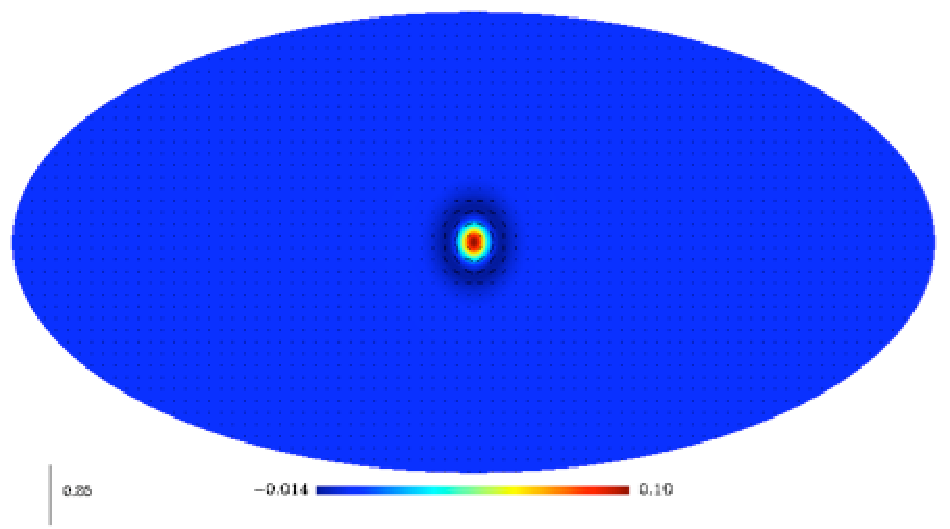
\includegraphics[width=7cm]{fig_e_iwt_back_scale2.pdf}
 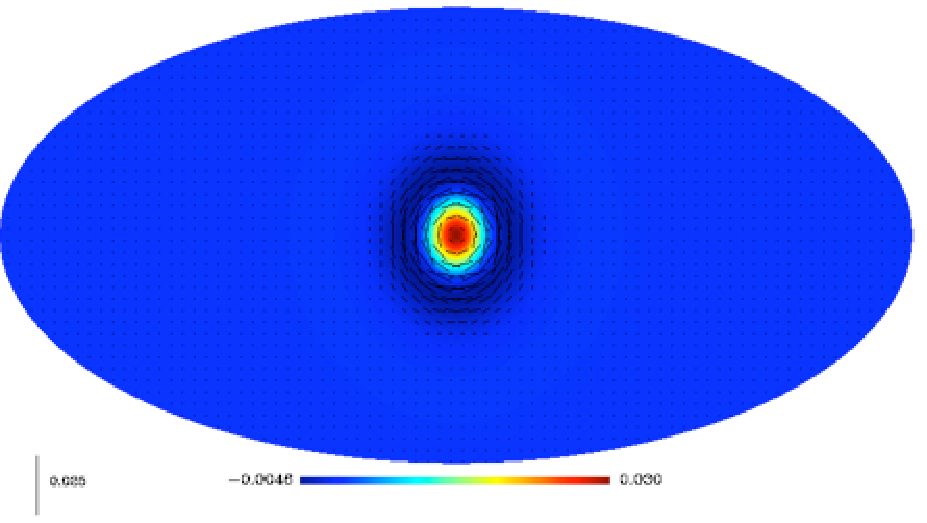
\includegraphics[width=7cm]{fig_b_iwt_back_scale2.pdf}
 }
  \hbox{
 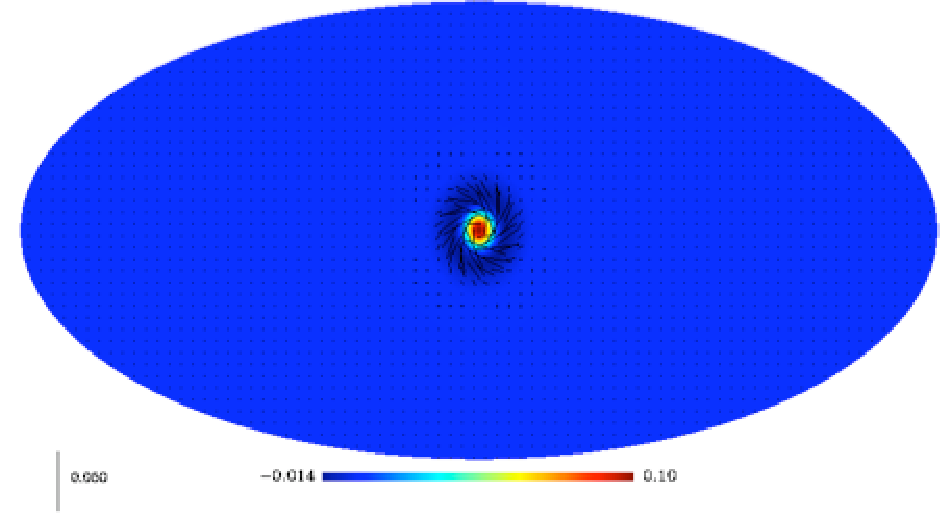
\includegraphics[width=7cm]{fig_e_iwt_back_scale3.pdf}
 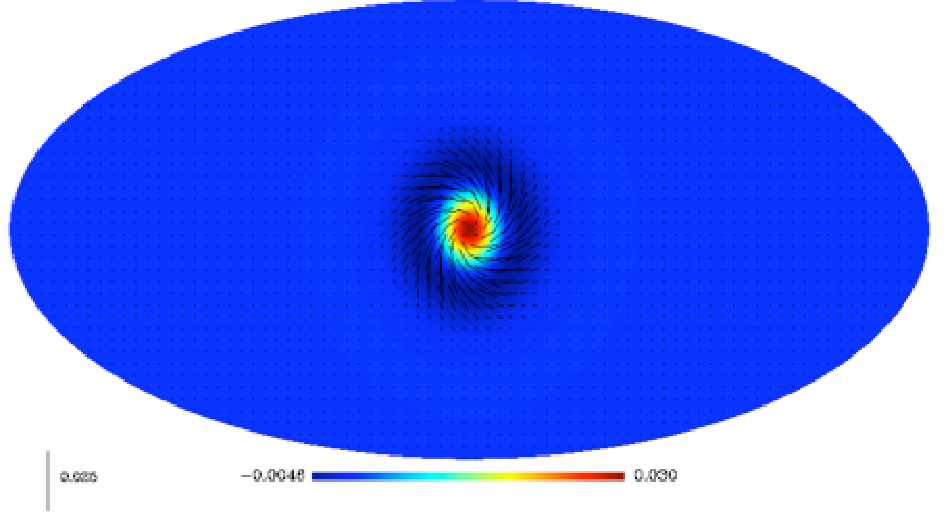
\includegraphics[width=7cm]{fig_b_iwt_back_scale3.pdf}
 }
 \hbox{
 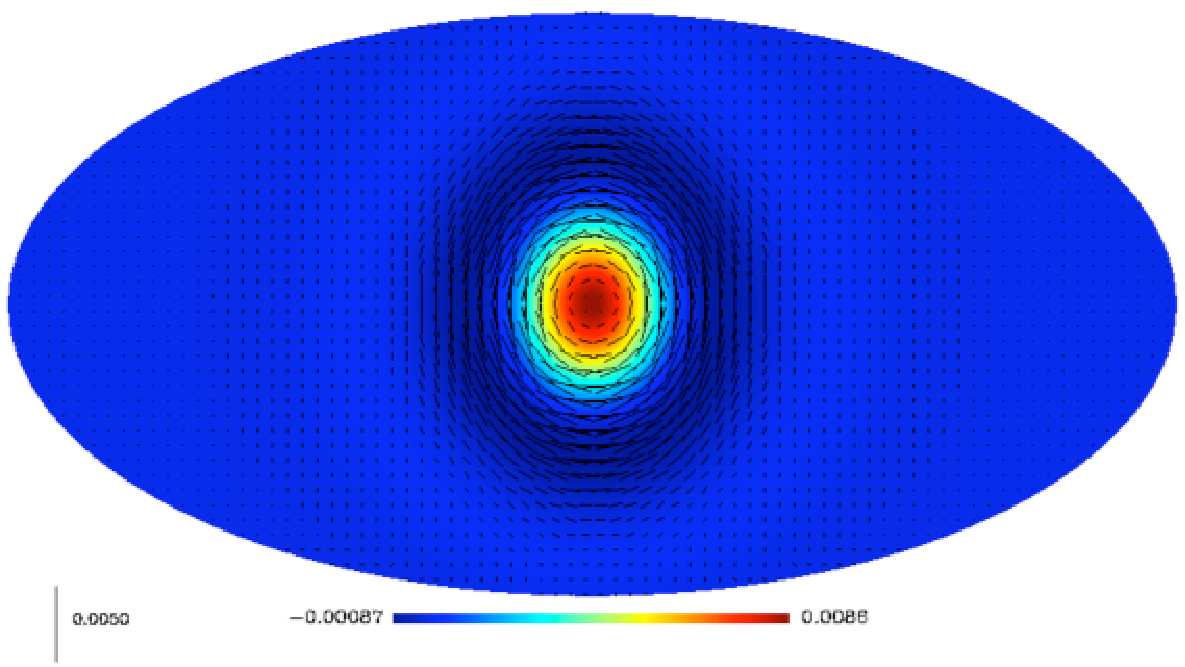
\includegraphics[width=7cm]{fig_e_iwt_back_scale4.pdf}
 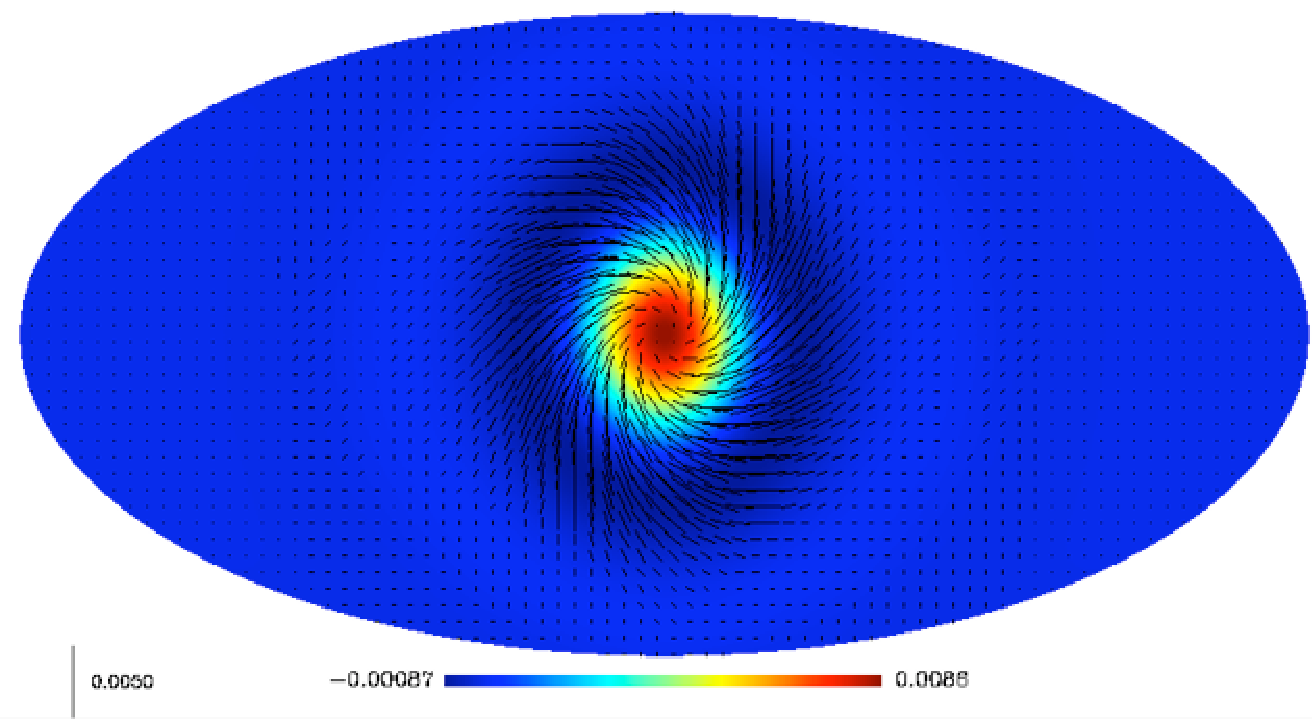
\includegraphics[width=7cm]{fig_b_iwt_back_scale4.pdf}
 }
 }
 }
\caption{E-isotropic wavelet transform backprojection (left) and B-isotropic wavelet backprojection (right).}
\label{fig_eb_iwt_back}
\end{figure*}
Obviously, the transform described above is invertible and the inverse transform is readily obtained by applying the inverse 
of each of the three steps in reverse order. If, as in the example decomposition above, we take the wavelet function to be 
the difference between two successive low pass approximations, the third step is inverted by simply summing the last low pass 
approximation with the maps of wavelet coefficients from all scales as in equation~\ref{IWT} : 
\begin{eqnarray}
T  & = & c_{J}^T + \sum_{j=1}^{J} w_j^T \quad \quad \nonumber \\
E & = & c_{J}^E + \sum_{j=1}^{J} w_j^E \quad \quad \nonumber \\
B & = &  c_{J}^B + \sum_{j=1}^{J} w_j^B
\end{eqnarray}
where $c_{J}^X$ stands for the low resolution approximation to component $X$ and $w_j^X$ is the map of wavelet coefficients of that component on scale $j$. Finally, noting that : 
\begin{eqnarray}
Q  & =  & -\frac{1}{2} \sum_{\ell, m}   a_{\ell m} ^E   ( {_{ 2} Y}_{\ell m} +  {_{ -2} Y}_{\ell m} ) +  i a_{\ell m} ^B ( {_{ 2} Y}_{\ell m} -  {_{ -2} Y}_{\ell m} )  \nonumber \\
     & =  & \sum_{\ell, m}   a_{\ell m} ^E   Z_{\ell m}^+ +  i a_{\ell m} ^B Z_{\ell m}^-   \\ \nonumber
U  & =   & -\frac{1}{2} \sum_{\ell, m}   a_{\ell m} ^B   ( {_{ 2} Y}_{\ell m} +  {_{ -2} Y}_{\ell m} ) -  i a_{\ell m} ^E ( {_{ 2} Y}_{\ell m} -  {_{ -2} Y}_{\ell m} )  \nonumber \\
      & =  & \sum_{\ell, m}   a_{\ell m} ^B Z_{\ell m}^+ -  i a_{\ell m} ^E Z_{\ell m}^-   
\end{eqnarray}
the initial representation of the polarized data in terms of $T$, $Q$ and $U$ maps is reconstructed from its wavelet coefficients using the following equations : 
% \begin{eqnarray}
%T= c_{J}^T + \sum_{j=1}^{J} w_j^T \\ \nonumber
%Q = \Big \{ \sum_{\ell, m}   <  c_{J}^E , Y_{\ell m}>  {_{ +} Z}_{\ell m} +  i <  c_{J}^B , Y_{\ell m}>  {_{ -} Z}_{\ell m} \Big \}        +   \sum_{j=1}^{J}  \Big \{ \sum_{\ell, m}  <  w_j^E , Y_{\ell m}>  {_{ +} Z}_{\ell m} +  i <  w_j^B , Y_{\ell m}>  {_{ -} Z}_{\ell m} \Big \}    \\ \nonumber 
%U = \Big \{ \sum_{\ell, m}   <  c_{J}^B , Y_{\ell m}>  {_{ +} Z}_{\ell m}  -  i <  c_{J}^E , Y_{\ell m}>  {_{ -} Z}_{\ell m} \Big \}        +   \sum_{j=1}^{J}  \Big \{ \sum_{\ell, m}  <  w_j^B , Y_{\ell m}>  {_{ +} Z}_{\ell m} -  i <  w_j^E , Y_{\ell m}>  {_{ -} Z}_{\ell m} \Big \}    
%\end{eqnarray}
%\begin{eqnarray}
%T =& c_{J}^T + \sum_{j=1}^{J} w_j^T \\ \nonumber
%Q =& c_{J}^E  \sum_{\ell, m} Y_{\ell m}^{\dagger} Z_{\ell m}^+ + i c_{J}^B  \sum_{\ell, m} Y_{\ell m} ^{\dagger} Z_{\ell m}^-  +   \sum_{j=1}^{J}  \Big \{  w_j^E  \sum_{\ell, m} Y_{\ell m}^{\dagger} Z_{\ell m}^+ +{i} w_j^B  \sum_{\ell, m} Y_{\ell m}^{\dagger}  Z_{\ell m}^- \Big \}    \\ \nonumber 
%U =& c_{J}^B  \sum_{\ell, m} Y_{\ell m}^{\dagger} Z_{\ell m}^+ -  i c_{J}^E  \sum_{\ell, m} Y_{\ell m} ^{\dagger} Z_{\ell m}^-  +   \sum_{j=1}^{J}  \Big \{  w_j^B  \sum_{\ell, m} Y_{\ell m}^{\dagger} Z_{\ell m}^+ - {i} w_j^E  \sum_{\ell, m} Y_{\ell m}^{\dagger}  Z_{\ell m}^- \Big \}   
%\end{eqnarray}
\begin{eqnarray}\label{eq:recons}
T =& c_{J}^T + \sum_{j=1}^{J} w_j^T \\ \nonumber
Q =& c_{J}^{E,+} + i c_{J}^{B,-} + \sum_{j=1}^{J} \Big \{ w_j^{E,+} + i w_j^{B,-} \Big \} \\ \nonumber 
U =& c_{J}^{B,+} - i c_{J}^{E,-} + \sum_{j=1}^{J} \Big \{ w_j^{B,+} - i w_j^{E,-} \Big \}
\end{eqnarray}
where
\begin{eqnarray}\label{eq:change}
c_{J}^{X,+} = c_{J}^X \sum_{\ell, m} Y_{\ell m}^{\dagger} Z_{\ell m}^+ \quad \textrm{and} \quad c_{J}^{X,-} = c_{J}^X \sum_{\ell, m} Y_{\ell m}^{\dagger} Z_{\ell m}^- 
\end{eqnarray}
with $W^\dagger$ denoting the transpose conjugate of $W$ so that $\tilde{W} W^\dagger$ is the scalar dot product of $\tilde{W}$ and $W$ 
while $W^\dagger \tilde{W}$ is an operator (or matrix) acting on its left hand side as a projection along $W$ and \emph{reconstruction} 
along $\tilde{W}$. In practice, the Healpix software package provides us with an implementation of the forward and inverse spin $0$ and 
spin $2$ spherical harmonics transforms which we need to implement the proposed inverse transform given by equations~\ref{eq:recons} 
and~\ref{eq:change}. Clearly, as mentioned earlier in section~\ref{sec:UWTS}, we could have chosen some other wavelet function than merely 
the difference between two consecutive scaling functions, and the transformation would still be nearly as simple to invert. Fig.\ref{fig_eb_iwt_back} 
shows, on the left, backprojections of E-wavelet coefficients, and, on the right, backprojections of B-wavelet coefficients on the right hand side at different scales.

%---------------------------------------------------------------------------------------------------------------------------------------
\subsection*{E-B  Curvelet}
%---------------------------------------------------------------------------------------------------------------------------------------
\begin{figure*}[htb]
\centerline{
\vbox{
 \hbox{
 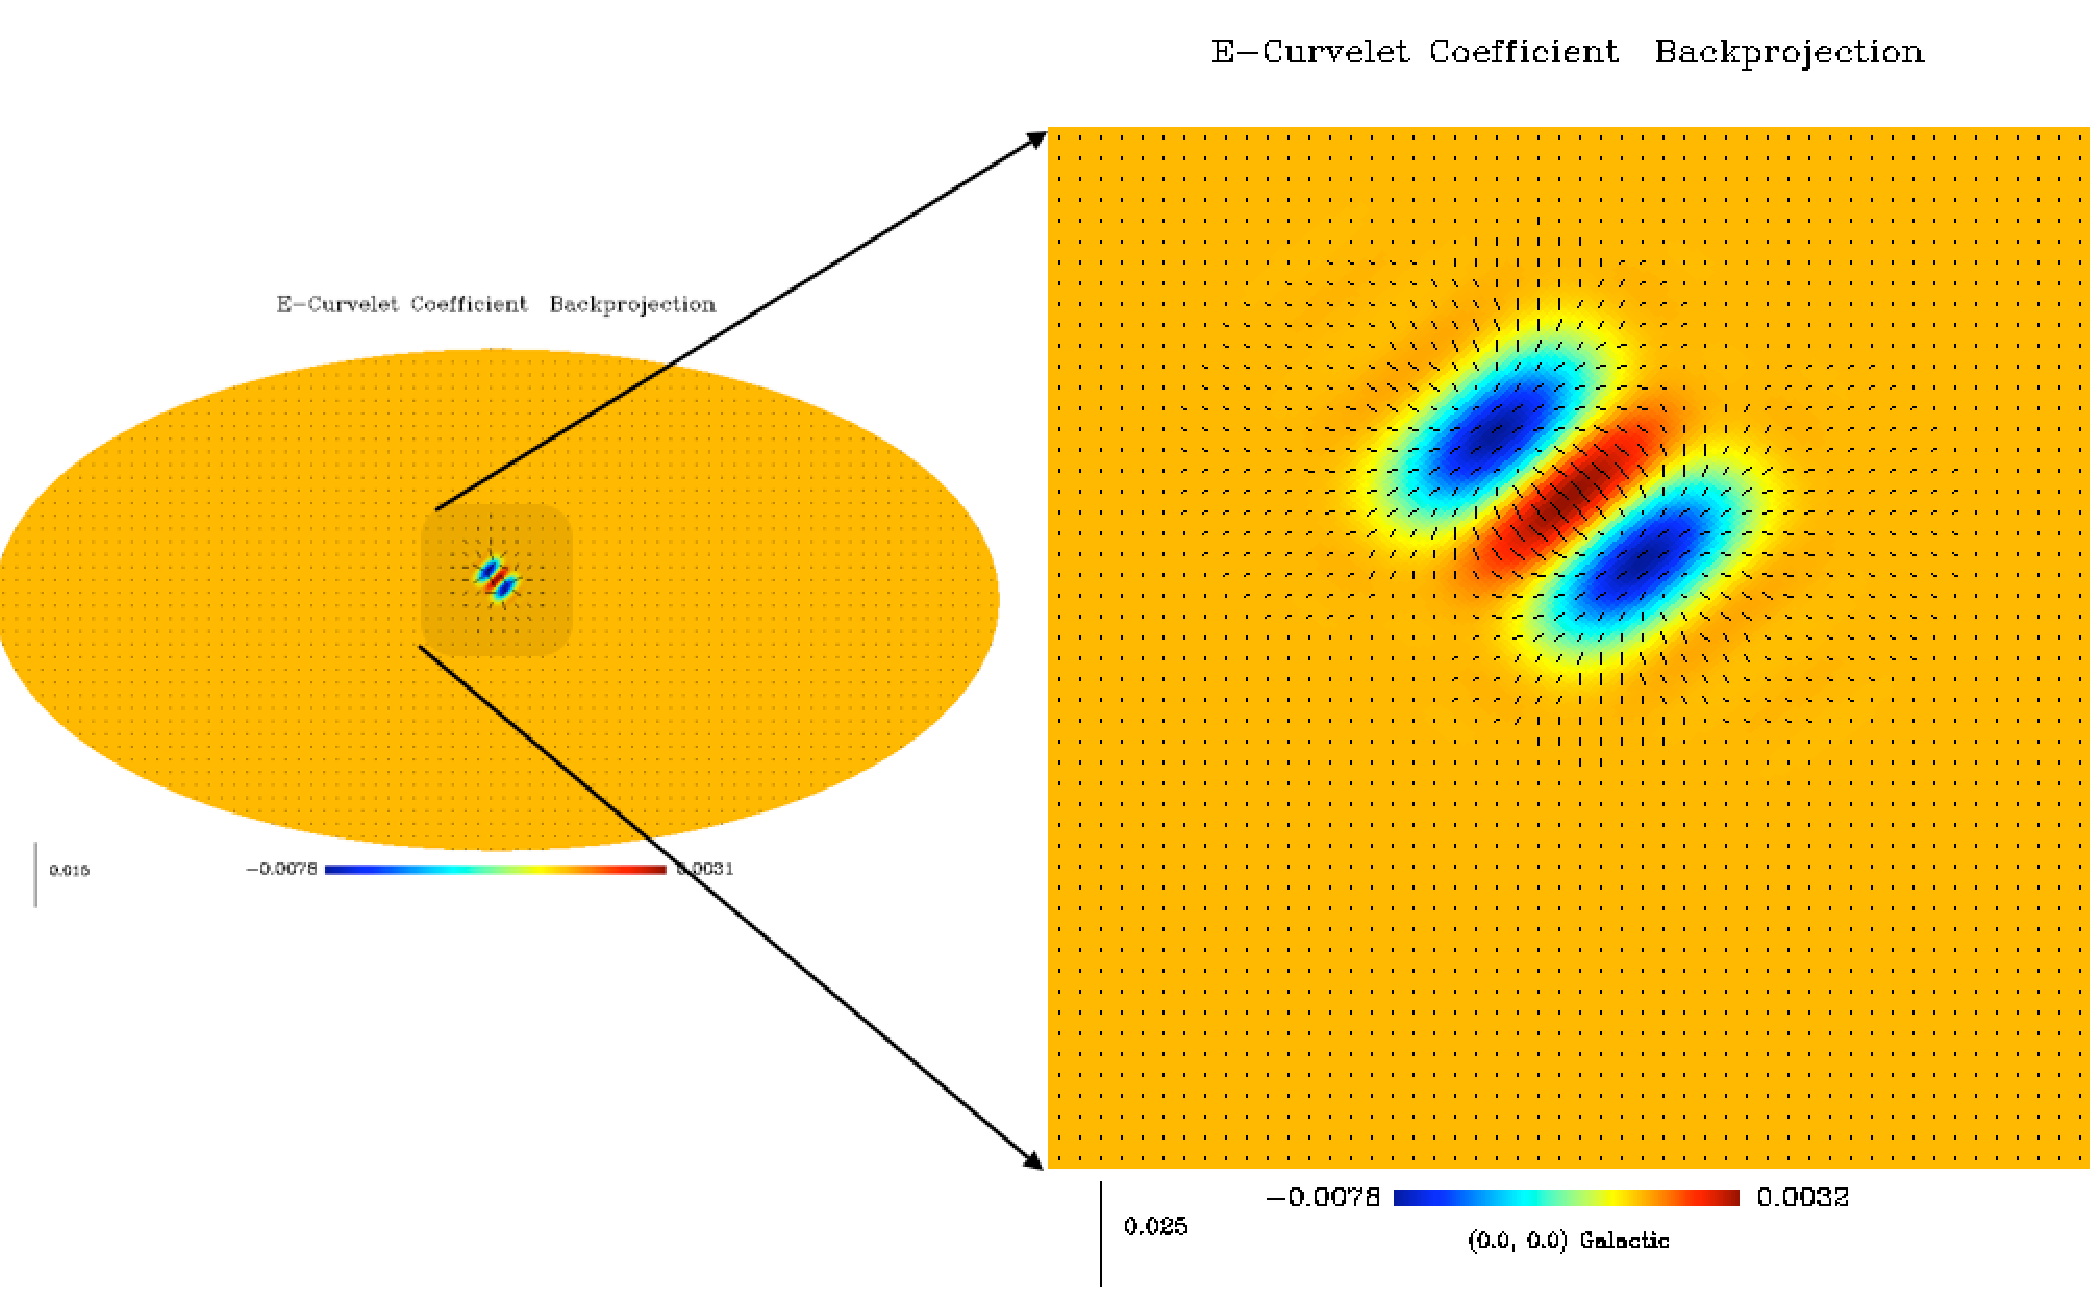
\includegraphics[width=12cm]{fig_ecur_back.pdf}
 }
  }
 }
\caption{E-curvelet coefficient backprojection.}
\label{fig_ecur_back}
\end{figure*}

\begin{figure*}[htb]
\centerline{
\vbox{
 \hbox{
 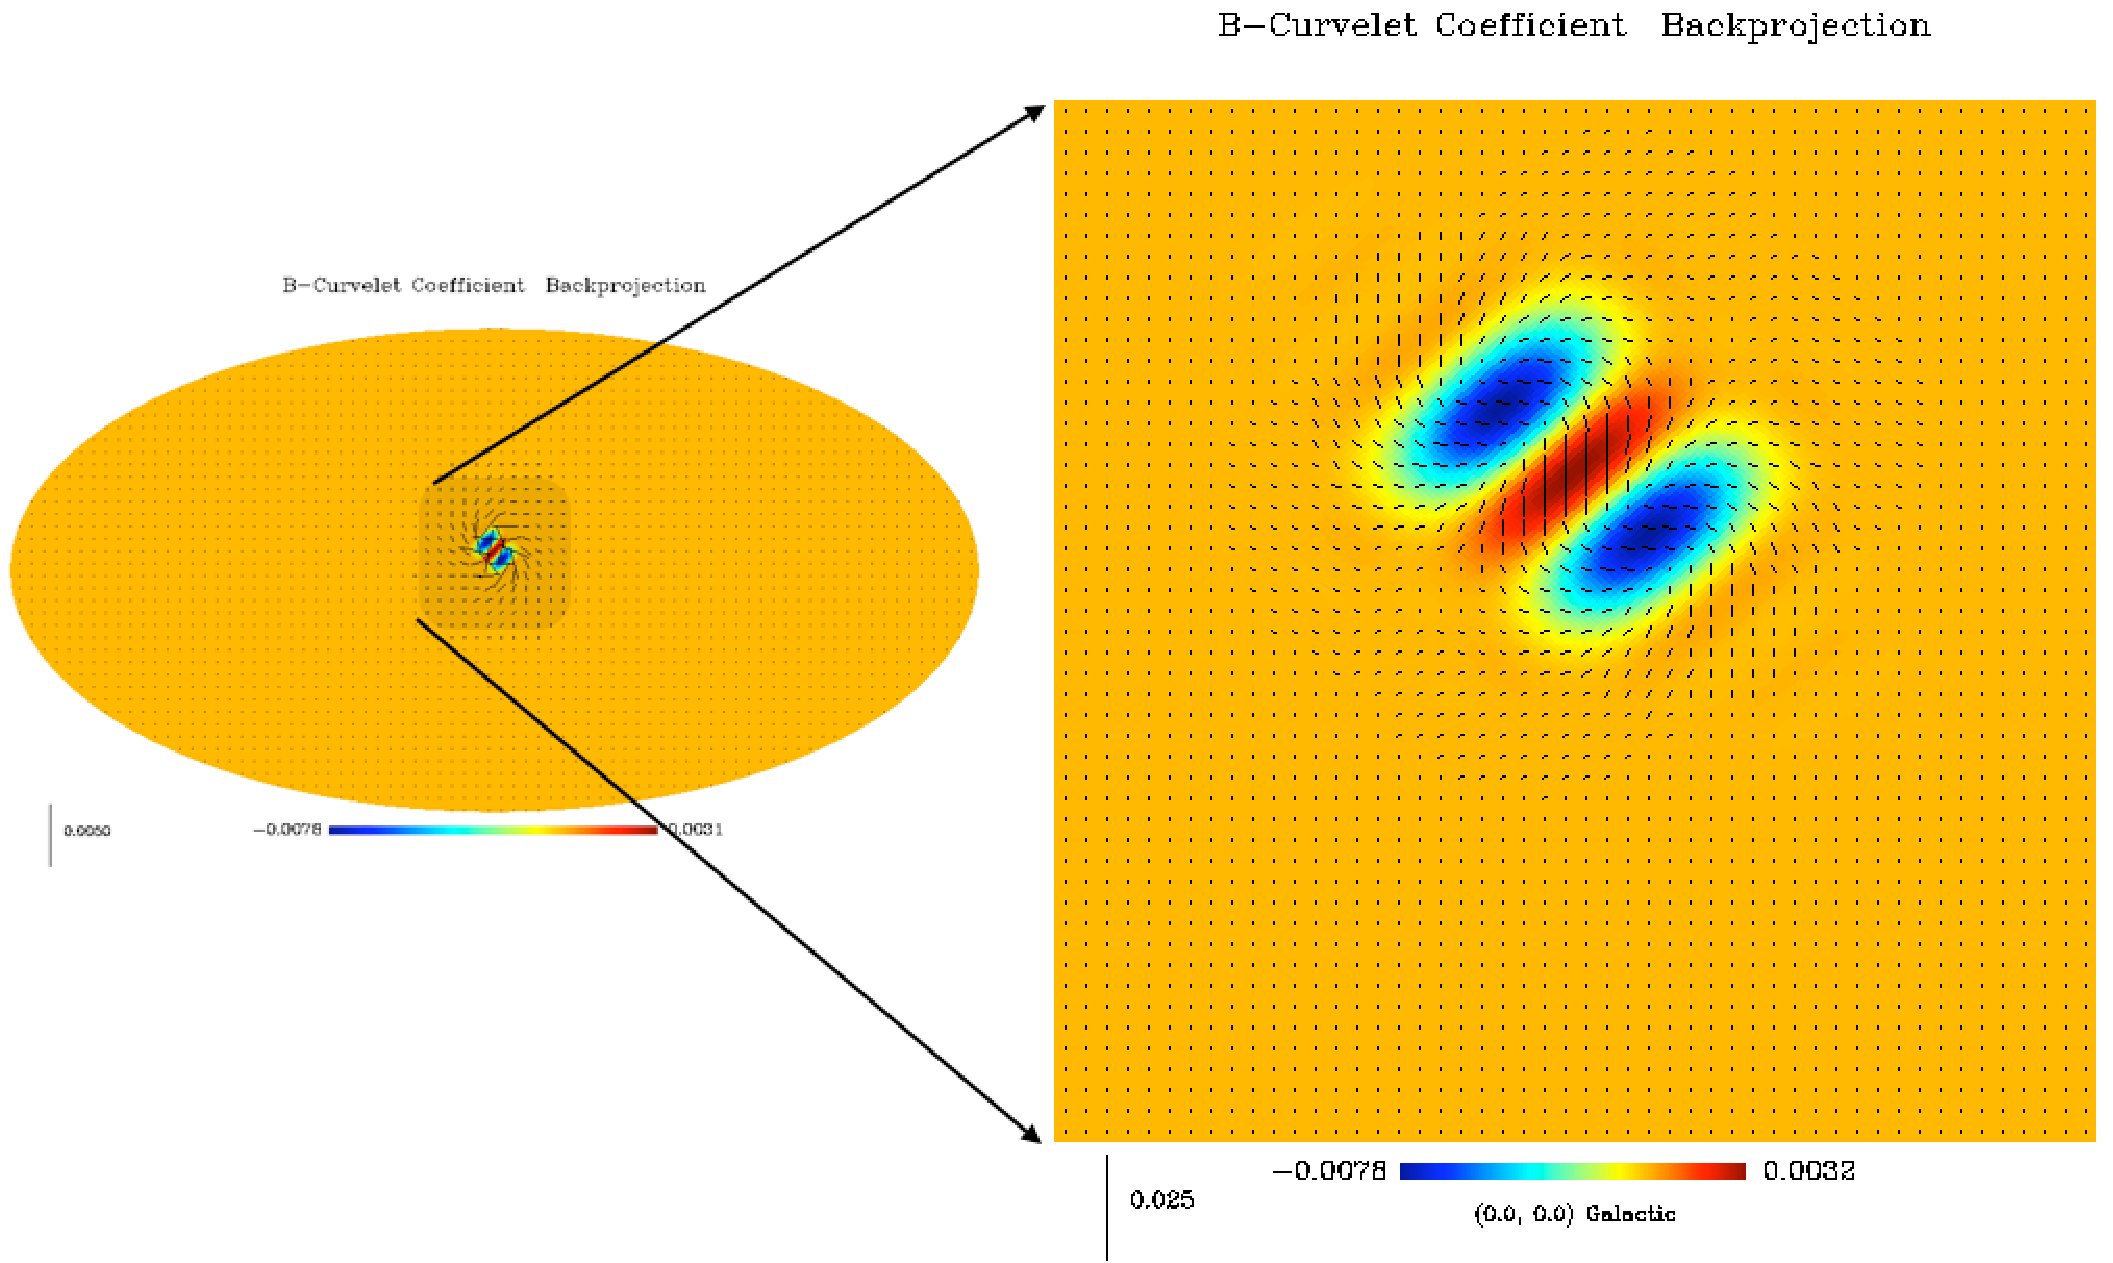
\includegraphics[width=12cm]{fig_bcur_back.pdf}
 }
 }
 }
\caption{B-curvelet coefficient backprojection.}
\label{fig_bcur_back}
\end{figure*}
Similarly to the EB-wavelet constructions, we can easily construct an EB-curvelet transform by first computing the E and B components using 
the spin $\pm 2$ spherical harmonics transform, and then applying a curvelet transform on the sphere separately on each of these two components.
Fig.~\ref{fig_ecur_back} shows the backprojection of an E-curvelet coefficient and Fig.~\ref{fig_bcur_back} shows the backprojectionof a B-curvelet coefficient.

%---------------------------------------------------------------------------------------------------------------------------------------


% Filtering chapter


\chapter{Blind Source Separation on the Sphere}
\label{ch_mrs_ica}

\section{Introduction}
\index{blind source separation}
\index{ICA}

Blind Source Separation (BSS) is a problem that occurs in multi-dimensional data processing. The overall goal is to recover 
unobserved signals, images or sources $S$ from mixtures of these sources $X$ observed typically at the output of an 
array of sensors. The simplest mixture model takes the form:
\begin{equation}\label{model0}
X = A S
\end{equation}
where $X$ and $S$ are random vectors of respective sizes $m \times 1$, $n \times 1$ and $A$ is an $m \times n$ matrix. The 
entries of $S$ are assumed to be independent random variables. Multiplying $S$ by $A$ linearly mixes the $n$ sources into 
$m$ observed processes. \\ 
   
Independent Component Analysis methods were developed to solve the BSS problem, i.e. given a batch of $T$ observed 
samples of $X$, estimate the mixing matrix $A$ and reconstruct the corresponding $T$ samples of the source vector $S$, relying 
mostly on the statistical independence of the source processes. Note that with the above model, the independent sources can 
only be recovered up to a multiplication by a non-mixing matrix i.e. up to a permutation and a scaling of the 
entries of $S$. Although independence is a strong assumption, it is in many cases physically plausible. The point is that 
it goes beyond the simple second order decorrelation obtained for instance using Principal Component Analysis (PCA) : decorrelation 
is not enough to recover the source processes since any rotation of a white random vector remains a white random vector.\\

Algorithms for blind component separation and mixing matrix estimation depend on the model used for the probability distribution 
of the sources. In a first set of techniques, source separation is achieved in a noise-less setting, based on the 
non-Gaussianity of all but possibly one of the components. Most mainstream Independent Component Analysis (ICA)  techniques belong to this category : JADE~\citep{ica:jade}, 
FastICA, Infomax~\citep{ica:icabook}. In a second set of blind techniques, the components are modeled as Gaussian processes, either 
stationary or non stationary and, in a given representation, separation requires that the sources have diverse, i.e. non 
proportional, variance profiles. The Spectral Matching ICA method (SMICA) ~\citep{ica:Del2003}, considers in this sense the case of 
mixed stationary Gaussian components and goes further than the above model Eq.~\eqref{model0} by taking into account additive 
instrumental noise $N$:
\begin{equation}\label{model1}
X = A S + N
\end{equation}
Moving to a Fourier representation, the idea is that colored components can be separated based on the diversity of their power spectra.\\ 
 
The next  section give a short overview of two significant ICA methods mentioned above and implemented in the \mrs package: 
JADE  and FastICA ~\citep{ica:icabook}. 
This is followed by a description of ways to 
combine wavelets and ICA techniques. Some useful properties of wavelet transforms can indeed come enhance the performance of ICA  methods in several situations. 
Finally, we present the method GMCA, which performs a blind source separation using the the sparsity concept.
    
\section{JADE}
\index{ICA!jade}

The Joint Approximate Diagonalization of Eigenmatrices method (JADE) assumes the observed data $X$ follows the noiseless mixture 
model~\eqref{model0} where the independent sources $S$ are non-Gaussian i.i.d.\footnote{The letters i.i.d. stand for 
independently and identically distributed meaning that each entries of $X$ at a given time $t$ are independent of $X$ at any other 
time $t'$ and that the distribution of $X$ does not depend on time.} random processes. The mixing matrix is assumed to be square 
and invertible so that (de)mixing is actually just a change of basis.

As mentioned above, second order statistics do not retain enough information for source separation in this context: finding a change of 
basis in which the data covariance matrix is diagonal will not in general enable to identify the independent sources properly. Nevertheless, 
decorrelation is half the job~\citep{ica:tutorial} and one may seek the basis in which the data is represented by maximally independent 
processes among those bases in which the data is decorrelated. This leads to so-called orthogonal algorithms: after a proper whitening of 
the data by multiplication with the inverse of a square root of the covariance matrix of the data $W$, one is then seeking a rotation $R$ 
(which leaves things white) so that $\hat{ S}$ defined by
\begin{equation}
\hat{ S} = W^{-1} \, Y =  W^{-1}\, R \, X_{\textrm{white}}  = W^{-1}\, R \, W \, X 
\end{equation}
and $\hat{B} = \widehat{A^{-1}} =  W^{-1}\, R \, W$ are estimations of the sources and of the inverse of the mixing matrix.\\

JADE is such an orthogonal ICA method and, like most mainstream ICA techniques, it exploits higher order statistics so as to achieve some 
sort of non linear decorrelation. Precisely, in the case of JADE, statistical independence is assessed using fourth order cross cumulants : 
%\begin{eqnarray} \nonumber	 
%F_{ijkl} & = & \textrm{cum}( y_i, y_j, y_k, y_l ) \nonumber \\
%  & = & \mathcal{E} (y_i y_j y_k y_l) - \mathcal{E} (y_i y_j)\mathcal{E} (y_k y_l) \nonumber \\
%  & & -\mathcal{E} (y_iy_l)\mathcal{E} ( y_j y_k)-\mathcal{E} (y_iy_k)\mathcal{E} (y_j y_k)
%\end{eqnarray}
\begin{eqnarray} \nonumber
F_{ijkl} & = & \textrm{cum}( y_i, y_j, y_k, y_l ) \nonumber \\
 & = & \mathcal{E} (y_i y_j y_k y_l) - \mathcal{E} (y_i y_j)\mathcal{E} (y_k y_l) -\mathcal{E} (y_iy_l)\mathcal{E} ( y_j y_k)-\mathcal{E} (y_iy_k)\mathcal{E} (y_j y_k)
\end{eqnarray}
where $\mathcal{E}$ stands for statistical expectation and the $y_i$'s are the entries of vector $Y$ modeled as random variables, 
and the correct change of basis (i.e. rotation) is found by somehow diagonalizing the fourth order cumulant tensor. 
Indeed, if the $y_i$'s were independent, all the cumulants with at least two different indices would be zero. As a consequence of 
the independence assumption of the source processes $S$ and of the whiteness of $Y$ for all rotations $R$, the fourth order 
tensor $F$ is well structured: JADE was precisely devised to take advantage of the algebraic properties of $F$. JADE's objective 
function is given by
\begin{eqnarray}  \nonumber	 
%\mathcal{J}_{\textrm{jade}}( R )   &=& \sum _{ijkl \ne ijkk}  \textrm{cum}(  y_i, y_j, y_k, y_l )^2  \nonumber    \\
  \mathcal{J}_{\textrm{jade}}( R ) & =&  \sum _{ij}   \sum_{k \ne l} \textrm{cum}(  y_i, y_j, y_k, y_l )^2  
\end{eqnarray}
which can be interpreted as a joint diagonalization criterion. Fast and robust algorithms are available for the minimization 
of $\mathcal{J}_{\textrm{jade}}( R )$ with respect to $R$ based on Jacobi's method for matrix diagonalization~\citep{ica:pham2001}. 
More details on JADE can be found in~\citep{ica:jade,ica:tutorial,ica:icabook}.


\subsubsection{JADE for spherical maps}

Applying JADE on multichannel data mapped to the sphere does not require any particular modification of the algorithm. Indeed, JADE estimates 
the fourth order cumulant tensor from the available data samples assuming an i.i.d. random field. Hence, given a pixelization scheme on 
the sphere such as provided by the Healpix package, JADE can be directly applied to the multichannel spherical data pixels.


\section{FastICA}
\index{ICA!fastica}

FastICA is by now a standard technique in ICA. Like JADE, it is meant for the analysis of mixtures of independent non-Gaussian sources in 
a noise-less setting. A complete description of this method can be found in \citep{ica:icabook} and references therein\footnote{Many papers on this 
algorithm are available at http://www.cs.helsinki.fi/u/ahyvarin/papers/fastica.shtml}. We give here a brief and simplified account 
of the algorithm. FastICA, again like JADE, is a so-called orthogonal ICA method: the independent components are sought by maximizing a 
measure of non-Gaussianity under the constraint that they are decorrelated. Intuitively, one should understand that mixtures of independent 
non-Gaussian random variables tend to look more Gaussian. An enlightening view on the relation between mutual information, which is 
a natural measure of independence, decorrelation and non-Gaussianity can be found in~\citep{ica:3easy,ica:geomindep}. Non-Gaussianity is assessed 
in FastICA using a contrast function $G$ based on a non-linear approximation to negentropy~\citep{ica:icabook}. In practice, depending 
on the application, different approximations or non-linear (non-quadratic) functions should be experimented with. In a simple deflation scheme, 
for sphered data, the directions are found sequentially : a direction $r$ of maximal non-Gaussianity is sought by maximizing
\begin{equation}
J_G(r) = \Big( \mathcal{E} \{ G(r^T x_{\textrm{white}}  ) \} - \mathcal{E} \{ G(\nu ) \} \Big)^2 
\end{equation}
where $\nu$ stands for centered unit variance Gaussian variable, under the constraint that $r$ has unit norm and that $r$ is orthogonal 
to the directions found previously.\\ \\
The contrast function $G$ can for instance be chosen among the following~\citep{ica:icabook}:
\begin{eqnarray}
G_0 (u)  & = &  \frac{1}{a} \textrm{log}\,\textrm{cosh} (a u ) \nonumber    \\
G_1 (u)  & = &  -\frac{1}{a} \textrm{exp}(- a u^2 / 2 )   \nonumber	   \\
G_2 (u)  & = &  \frac{1}{4} u^4 \nonumber    \\
\end{eqnarray}
where $a$ is a constant to be determined depending on the application. It can be shown that the maxima of $J_G$ occur at certain maxima 
of $\mathcal{E} \{ G(r^T x_{\textrm{white}} ) \} $. These are obtained for $r$ solution to :
\begin{equation}
\mathcal{E} \{ x_{\textrm{white}} g(r^T x_{\textrm{white}}  ) \} - \lambda r = 0 
\end{equation}
where $\lambda$ is a constant easily expressed in terms of the optimal direction $r_0$, and $g$ is the derivative of $G$. Solving this 
equation using Newton's method, and a few approximations, a fixed-point algorithm is derived which consists in repeating the 
following two steps until convergence :
\begin{eqnarray}
r  & \leftarrow & \mathcal{E} \{ x_{\textrm{white}} g(r^T x_{\textrm{white}}  ) \} - \mathcal{E} \{ g'(r^T x_{\textrm{white}}  ) \} r     \nonumber  \\
r  & \leftarrow  &  \frac{r}{\| r \|}   \nonumber	   \\
\end{eqnarray}
A simple implementation of this algorithm is included in the present package. It is largely based on the $\textbf{Matlab}^{TM}$ code 
available at www.cis.hut.fi/projects/ica/fastica/. 

 
\section{Wavelet and BSS} 
\index{wavelet!ICA}
\index{ICA!wavelet}

\label{sec:wjade}
\index{ICA!wjade}
\index{jade!wavelet}

Wavelets come into play as a sparsifying transform. Applying a wavelet transform on both sides of~\eqref{model0} does not affect the 
mixing matrix and the model structure is preserved. Also, moving the data to a wavelet representation does not affect its information 
content. However, the statistical distribution of the data coefficients in the new representation is different: wavelets are known to 
lead to sparse i.i.d. representations of structured data. Further, the local (coefficient wise) signal to noise ratio 
depends on the choice of a representation. A wavelet transform tends to grab the informative coherence between pixels while averaging 
the noise contributions, thus enhancing structures in the data. Although the standard ICA model~\eqref{model0} is for a noiseless setting, 
the derived methods can be applied to real data. Performance will depend on the detectability of significant coefficients i.e. on 
the sparsity of the statistical distribution of the coefficients. Moving to a wavelet representation will often lead to more robustness to noise.    

Once the data has been transformed to a proper representation (e.g. wavelets but also ridgelets and curvelets in the case of strongly 
anisotropic 2D or 3D data), WJADE (resp. WFastICA) consists in applying the standard JADE (resp. FastICA) method to the new multichannel coefficients. Once the mixing matrix 
is estimated, the initial source maps are obtained using the adequate inverse transform after some non linear denoising or thresholding of 
the coefficients if necessary.


\section{Sparse Blind Source Separation: the GMCA method}
% \section{Generalized Morphological Component Analysis on the sphere}
\label{sec:gmca}

\subsection{Morpho-Spectral Diversity}
%\label{sec:morph-spec-diversity}
Extending the redundant representation framework to the multichannel case requires defining what a multichannel overcomplete representation is.
Let us assume in this section that $\A = [\varphi_{\nu,1}, \cdots, \varphi_{\nu, N_c}] \in \RR^{N_c \times N_s}$ is a \textit{known spectral} dictionary, 
and $\W = [ \varphi_{1}, \cdots, \varphi_{T}] \in \RR^{N \times T}$ is a \textit{spatial} or \textit{temporal} dictionary\footnote{The adjectives 
\textit{spectral} and \textit{spatial} that characterize the dictionaries are not formal. Owing to the symmetry of the multichannel sparse decomposition problems, 
$\A$ and $\W$ have no formal difference. In practice and more particularly in multi/hyperspectral imaging, $\A$ will refer to the dictionary of physical spectra 
and $\W$ to the dictionary of image/signal waveforms. In the BSS problem, $\A$ is unknown.}. We assume that each source $s_i$ can be represented as 
a (sparse) linear combination of atoms in $\W$; $s_i=\W\alpha_i$. Let $\balpha$ the $N_s \times T$ matrix whose rows are $\alpha_i^\Tr$.

From Eq.~\eqref{model0}, the multichannel noiseless data $\bY$ can be written as
\be
\label{eq:tensor1}
\bY = \A\balpha\W^\Tr = \sum_{i=1}^{N_s}\sum_{j=1}^{T} \parenth{\varphi_{\nu,i}\varphi_{j}^\Tr}\alpha_i[j] ~.
\ee
Consequently, each column in of $\bY$ reads
\be
\label{eq:tensor2}
\bY[.,l] = \parenth{\A \otimes \W[l,.]} \mathrm{vect}(\balpha) ~, \quad \forall ~ l=1,\cdots,N ~,
\ee
and finally
\be
\label{eq:tensor3}
\mathrm{vect}(\bY) = \parenth{\A \otimes \W} \mathrm{vect}(\balpha) ~,
\ee
where $\otimes$ is the tensor (Kronecker) product and the operator $\mathrm{vect}$ stacks the columns of its argument in a long 1D vector. 
This latter equation brings a clear and simple insight: the sparsity of the sources in $\W$ translates into sparsity of the multichannel data 
$\bY$ in the multichannel tensor product dictionary ${\bf \Psi}=\A \otimes \W$. 

The multichannel dictionary $\bf \Psi$ can also be seen as concatenation of multichannel atoms ${\bf \Psi}^{(ij)}=\varphi_{\nu,i}\varphi_{j}^\Tr$ 
which are rank-one matrices obtained from each atomic spectrum $\varphi_{\nu,i}$ and each spatial elementary atom $\varphi_{j}$ (see Eq.~\eqref{eq:tensor1}). 

Some of the popular recovery results in sparse component analysis algorithm rely on the mutual coherence of 
the dictionary~\citep{cur:elad02,miki:Gribonval-Nielsen,mca:Donoho-Elad}. In the multichannel case a quantity 
of that kind can be defined. In fact, by standard properties of the tensor product, one can easily show that 
the Gram matrix of a tensor product is the tensor product of the Gram matrices. Thus the mutual coherence of the multichannel dictionary $\bf \Psi$ is:
\index{coherence}
\begin{equation}
\label{eq:mmc}
0 \le \mu_{\bf \Psi}  =  \max\left\{\mu_{\A},\mu_{\W}\right\} < 1 ~ .
\end{equation}

This expression of mutual coherence is instructive as it tells us that multichannel atoms can be distinguished 
based on their spatial or spectral morphology. In other words, discriminating two multichannel atoms $\Psi_{ij}$ and $\Psi_{i'j'}$ may put on different faces:
\begin{itemize}
\item{Spatial or temporal (respectively spectral) diversity:} in this case $i=i'$ and $j \neq j'$ (respectively $i \neq i'$ and $j = j'$). 
These atoms have the same spectrum (respectively, spatial shape) but one can discriminate between them based on their 
spatial (respectively, spectral) diversity. From \eqref{eq:mmc}, their coherence is lower than $\mu_{{\W}}$ (respectively $\mu_{{\A}}$). 
Disentangling these multichannel atoms can equivalently be done in \ref{ch_sca_datarest}.

\item{Both diversities:} $i \neq i'$ and $j \neq j'$, this seems to be a more favorable scenario to differentiate 
the atoms as they do not share neither the same spectrum nor the same spatial (or temporal) ``shape". Note that 
from \eqref{eq:mmc}, the coherence between these atoms in this case is lower than $\mu_{{\A}}\mu_{{\W}} \le \max\left\{\mu_{\A},\mu_{\W}\right\}$.
\end{itemize}

\subsection{Multichannel Sparse Decomposition}

We embark from Eq.~\eqref{eq:tensor1}, where the multichannel dictionary ${\bf \Psi}$ is supposed to be overcomplete, i.e. $NN_c < TN_s$. 
The goal is to recover the sparsest solution $\balpha$ from $\bY$ which requires solving:
\begin{equation}
\label{eq:multi_l0}
\min_{\balpha \in \RR^{N_s \times T}} \sum_{i=1}^{N_s}\norm{\alpha_i}_{0} \st \bY  = \A \balpha \W^\Tr.
\end{equation}
As justified in \ref{sect_mca}, this combinatorial problem can be replaced by its convex relaxation substituting the $\ell_1$ norm for the $\ell_0$ pseudo-norm, hence giving:
\begin{equation}
\label{eq:multi_l1}
\min_{\balpha \in \RR^{N_s \times T}} \sum_{i=1}^{N_s}\norm{\alpha_i}_{1} \st \bY  = \A \balpha \W^\Tr.
\end{equation}

As \eqref{eq:tensor3} is a vectorized monochannel form of \eqref{eq:tensor1}, what we are trying so do is actually to find 
the sparsest solution of a monochannel underdetermined system of linear equations where the solution is sparse in an 
overcomplete tensor product dictionary. Recovery properties of monochannel sparse decomposition by $\ell_1$ minimization 
were overviewed in chapter~\ref{ch_sca_datarest}. Therefore, if one is able to translate those identifiability criteria 
in the language of tensor product dictionaries, then we are done.

In particular, the coherence-based sparse recovery criterion given in \citep{DonohoHuo} is trivial to adapt owing to \eqref{eq:mmc}. 
Indeed, if $\bY$ is $k$-sparse in the multichannel dictionary ${\bf \Psi}$ with $k < C(\mu_{{\bf \Psi}}^{-1}+1)$ for some $C > 0$ (typically $C=1/2$), 
and the dictionary is sufficiently incoherent (both spectrally and spatially), then the solution of Eq.~\eqref{eq:multi_l1} is unique, 
is a point of equivalence of Eq.~\eqref{eq:multi_l0} and Eq.~\eqref{eq:multi_l1}, and the recovery is stable to bounded noise on $\bY$. 

Above, we addressed the multichannel sparse decomposition problem without assuming any constraint on the sparsity pattern 
of the different channels. It is worth however pointing out that sparse recovery conditions from multichannel measurements 
can be refined if some structured sparsity is hypothesized. For instance, for structured multichannel representation 
(e.g. sources with disjoint supports) \citep{GN05} provided coherence-based sufficient recovery conditions by solving Eq.~\eqref{eq:multi_l1}. 
One should note that despite apparent similarities, the multichannel sparse decomposition problem discussed here is conceptually 
different from the one targeting \textit{simultaneous} sparse recovery of multiple measurements vectors (MMV) considered by several authors, see e.g. 
\citep{CREK05,MalioutovMMV05,TroppMMV06,ChenHuo06,ArgyriouMMVLearning08,BachMMVLearning08,GribonvalMMV08,EldarMMV08,LouniciMMVLearning09,WainwrightMMV09}. 
The latter are not aware of any mixing process via $\A$, and their goal is to recover $\balpha$ from MMV $\bY=\balpha\W^\Tr$ in which 
the vectors $\alpha_i$, i.e. rows of $\balpha$, have a common sparsity pattern. However the MMV model can also be written 
$\mathrm{vect}(\bY^\Tr) = \parenth{\W \otimes \I} \mathrm{vect}(\balpha^\Tr)$ as in Eq.~\eqref{eq:tensor3}. The most widely used approach 
to solve the simultaneous sparse recovery problem with joint sparsity is to minimize a mixed $\ell_p-\ell_q$ norm of the form 
$\sum_{j=1}^T\parenth{\norm{\balpha[.,j]}_p^q}^{1/q}$ for $p \geq 1, 0 \leq q \leq +\infty$.

\subsection{Generalized Morphological Component Analysis}
\label{subsec:gmca}
We now turn to the BSS problem and highlight the role of sparsity and morphological diversity as a source of contrast to solve it. 
Towards this goal, we assume that the sources are sparse in the spatial dictionary $\W$ that is the concatenation of $K$ orthonormal bases 
$\parenth{{\W}_{k}}_{k=1,\cdots,K}$: $\W = \left[{\W}_{1},\cdots,{\W}_{K} \right]$. The restriction to orthonormal bases is only formal 
and the algorithms to be presented later still work in practice even with redundant sub-dictionaries $\W_k$. 

\newpage
The Generalized Morphological Component Analysis framework assumes a priori that each source is modeled as the linear combination 
of $K$ morphological components where each component is sparse in a specific basis:
\begin{eqnarray}
\label{eq:sourcecomponents}
\forall i \in \{1,\cdots,N_s\}; \qquad s_i & = & \sum_{k=1}^K x_{i,k} = \sum_{k=1}^K \W_k\alpha_{i,k} \\
& = & \W \alpha_i \qquad \mbox{ where } \alpha_i =  \left[\alpha_{i,1}^\Tr,\cdots,\alpha_{i,K}^\Tr \right]^\Tr ~ \nonumber
\end{eqnarray}
GMCA seeks an unmixing scheme, through the estimation of $\A$, which leads to the sparsest sources $\bf S$ in the dictionary $\W$. 
This is expressed by the following optimization problem written in the augmented Lagrangian form:
\begin{multline}
\label{eq:optimgmca}
\min_{{\A},\alpha_{1,1},\cdots,\alpha_{N_s,K}} \frac{1}{2}\norm{\bY - {\A}\balpha\W^\Tr}^2_{\mathrm{F}} + \lambda \sum_{i=1}^{N_s} \sum_{k=1}^K \norm{\alpha_{i,k}}_p^p \\ 
\st \norm{a_i}_2 = 1 ~ \forall i \in \{1,\cdots,N_s\} ~
\end{multline} 
where typically $p=0$ or its relaxed convex version with $p=1$, and $\norm{{\bf X}}_{\mathrm{F}}=\parenth{\trace({\bf X}^\Tr{\bf X})}^{1/2}$ is the Frobenius norm. 
The unit $\ell_2$-norm constraint on the columns of $\A$ avoids the classical scale indeterminacy of the product $\bf AS$ in \eqref{model1}. 
The reader may have noticed that the MCA problem in chapter~\ref{ch_sca_datarest} is a special case of the GMCA problem Eq.~\eqref{eq:optimgmca} 
when there is only one source $N_s=1$ and one channel $N_c=1$ (no mixing). Thus GMCA is indeed a multichannel generalization of MCA. 

The program \eqref{eq:optimgmca} is a notoriously difficult non-convex optimization problem even for convex penalties when $p \geq 1$. 
More conveniently, following \eqref{model0}, the product $\bf AS$ can be split into $N_s \cdot K$ multichannel morphological components: 
${\bf AS} = \sum_{i,k} a_i x_{i,k}^\Tr = \sum_{i,k} (a_i \alpha_{i,k}^\Tr) \W_k^\Tr$. Based on this decomposition, and inspired by 
the block-coordinate relaxation as for MCA, GMCA yields an alternating minimization algorithm to estimate iteratively one term at a time \citep{starck:bobin07}. 
We will show shortly that the estimation of each morphological component $x_{i,k} = \W_k\alpha_{i,k}$ assuming $\A$ and $x_{\{i',k'\} \neq \{i,k\} }$ 
are fixed is obtained by simple hard or soft thresholding for $p=0$ and $p=1$.

Define the $(i,k)^{\textrm{th}}$ multichannel marginal residual by:
\begin{equation}
\label{eq:gmca_resi}
{\bf R}_{i,k} = {\bY} - \sum_{i' \neq i}   \sum_{k'\neq k}    a_{i'} x_{i',k'}^\Tr ~
\end{equation} 
as the part of the data $\bY$ unexplained by the multichannel morphological component $a_i x_{i,k}^\Tr$. Estimating $x_{i,k} = \W_{k} \alpha_{i,k}$, 
assuming $\A$ and the other components $x_{(i',k') \neq (i,k)}$ are fixed, leads to the component-wise optimization problem:
\begin{equation}
\label{eq:componentwisephi}
\min_{x_{i,k} \in \RR^{N}} \frac{1}{2}\norm{{\bf R}_{i,k} - (a_i \alpha_{i,k}^\Tr)\W^\Tr}_{\mathrm{F}}^2 +  \lambda \norm{\alpha_{i,k}}_p^p ~
\end{equation}

Since here ${\W}_k$ is an orthogonal matrix, with calculations using proximity operators, it can be shown that the unique solution 
of Eq.~\eqref{eq:componentwisephi} is obtained by a hard ($p=0$) or soft ($p=1$) thresholding. Hence, the closed-form estimate of 
the morphological component $x_{i,k}$ is: 
\begin{equation}
\label{eq:st_update}
\tilde{x}_{i,k} = \Delta_{\W_k,\lambda^\prime} \parenth{\frac{1}{\norm{a_i}_2^2} {\bf R}_{i,k}^\Tr a_i} ~
\end{equation}
where $\lambda^\prime=\lambda/\norm{a_i}_2^2$ for soft thresholding and $\lambda^\prime=\sqrt{2\lambda}/{\norm{a_i}_2}$ for hard thresholding. 
The operator $\Delta_{{\bf D}, \lambda}(x)$ consists of (i) computing the coefficients of $x$ in the dictionary ${\bf D}$, (ii)
thresholding (soft or hard) the obtained coefficients with the threshold $\lambda$, and (iii) reconstructing from thresholded coefficients: 
\begin{equation}
\Delta_{{\bf D},\lambda}(x) = {\bf D} \Thres_{\lambda} \left( {\bf D}^\Tr x \right)
\end{equation}
$\Thres_{\lambda}$ is either a hard or a soft thresholding. When $\W_k$ is redundant, \eqref{eq:st_update} is only the first iteration 
of a forward-backward splitting recursion, and which should be used when $\W_k$ is overcomplete.
However in practice \eqref{eq:st_update} can still be used to save computation time.
\index{iterative!hard thresholding}
\index{iterative!soft thresholding}

Now, considering $\{a_{i'}\}_{i' \neq i}$ and all morphological components as fixed, and recalling that $N_c \geq N_s$, updating the column $a_i$ is then just a least-squares estimate
\begin{equation}
\label{eq:a_update}
\tilde{a}_i = \frac{1}{\norm{s_i}^2_2} \left({\bf Y} - \sum_{i' \neq i} a_{i'} s_{i'}^\Tr\right) s_i ~
\end{equation}
where $s_i = \sum_{k=1}^K x_{i,k}$. This estimate is then projected onto the unit sphere to meet the unit $\ell_2$-norm constraint in Eq.~\eqref{eq:optimgmca}.
The GMCA algorithm is summarized in Algorithm~\ref{algo_gmca}.

{\linespread{1}
\begin{algorithm}[htb]
\caption{GMCA algorithm.}
\label{algo_gmca}
\noindent{\bf Task:} Sparse Blind Source Separation.\\
\noindent{\bf Parameters:} The data $\bY$, the dictionary $\W=[\W_1 \cdots \W_K]$, number of iterations $\niter$, number of sources $N_s$ and channels $N_c$, stopping threshold $\lambda_{\min}$, threshold update schedule.\\
\noindent{\bf Initialization:} $x_{i,k}^{(0)} = 0$ for all $(i,k)$, $\A^{(0)}$ random and threshold $\lambda_0$.\\
\noindent{\bf Main iteration:} \\
\For{$t=1$ {\bf to} $\niter$}{
    \For{$i=1,\cdots,N_s$ }{
    \For{$k=1,\cdots,K$ }{
       Compute the marginal residuals: $${\bf R}_{i,k}^{(t)} = {\bY}- \sum_{(i',k') \neq (i,k)} {a}_{i'}^{{(t-1)}}{x}_{i',k'}^{{(t-1)}^\Tr}.$$
       Estimate the current component ${x}_{i,k}^{(t)}$ via thresholding with threshold $\lambda_t$:\\
       ${x}_{i,k}^{(t)} = \Delta_{\W_k, \lambda_t}\left({\bf R}_{i,k}^{{(t)}^\Tr}{a}_i^{{{(t-1)}}}\right)$.
    }
Update $i$th source $s_i^{(t)} = \sum_{k=1}^K x_{ik}^{(t)}$. \\
Update $a_i$ assuming $a_{i' \neq i}^{(t)}$ and the morphological components $ {x}_{i,k}^{(t)} $ are fixed~:\\
 $ {a}_i^{{(t)}} = \frac{1}{\|{s}_i^{(t)}\|_2^2} \left({\bY} - \sum_{i' \neq i}^{N_s} {a}_{i'}^{(t-1)} {s}_{i'}^{{(t)}^\Tr} \right){s}_i^{{(t)}}$ and normalize to a unit $\ell_2$ norm.
}
Update the threshold $\lambda_t$ according to the given schedule.\\
\lIf{$\lambda_t \leq \lambda_{\min}$} stop.
}
\noindent{\bf Output:} Estimated sources $\big(s^{(\niter)}_i\big)_{i=1,\cdots,N_s}$ and mixing matrix ${\A}^{(\niter)}$.
\end{algorithm}}

For $p=1$ and fixed threshold $\lambda$, Algorithm~\ref{algo_gmca} can be shown to converge to a stationary point, see \citep{Tseng01,bobin-gmca-cmb}. 
This point is not guaranteed to be even a local minimum of the energy, and this is even less clear for $p=0$. Thus, in the same vein as MCA, GMCA relies 
on a salient-to-fine strategy using a varying threshold to mitigate the problem of sensitivity to initialization. More precisely, GMCA first computes 
coarse versions of the morphological components for any fixed source $s_i$. These raw sources are estimated from their most significant coefficients in $\W$. 
Then, the corresponding column $a_i$ is estimated from the most significant features of $s_i$. Each source and its corresponding column of $\A$ are then 
alternately and progressively refined as the threshold decreases towards $\lambda_{\min}$. This particular iterative thresholding scheme provides robustness 
to noise and initialization by working first on the most significant features in the data and then progressively incorporating smaller details to finely 
tune the model parameters. GMCA can be used with either linear or exponential decrease of the threshold as for MCA.

If $\A$ were known and fixed, the GMCA would be equivalent to performing an MCA sparse decomposition of $\bY$ in the tensor product 
multichannel dictionary ${\A} \otimes \W$. But as GMCA also updates the mixing matrix at each iteration, it is able to learn the 
spectral part of the multichannel dictionary directly from the data.

\subsubsection{The Thresholding Strategy}

\index{iterative!hard thresholding}
\index{iterative!soft thresholding}

\paragraph*{Hard or soft thresholding?} In practice, it was observed that hard thresholding leads to better results \citep{starck:bobin06,starck:bobin07}. 
Furthermore, if $\A$ is known and no noise contaminates the data, GMCA with hard thresholding will enjoy the sparse recovery guarantees given in \citep{starck:bobin_2,BobinJMIV}, 
with the proviso that the morphological components are contrasted and sparse in a sufficiently incoherent multichannel dictionary ${\A} \otimes \W$. 
%Furthermore in \citet{starck:bobin_2}, it was shown empirically that the use of hard-thresholding is likely to provide the $\ell_0$ sparse solution for 
%the single channel sparse decomposition problem. By analogy, the use of a hard-thresholding operator is assumed to solve the multichannel $\ell_0$ quasi-norm 
%problem instead of \eqref{eq:optim_l1}. Recent results give also theoretical support to iterative hard thresholding methods \citep{blumensath08,blumensath09,maleki09,donoho09}.

\paragraph*{Handling additive Gaussian noise.}
The GMCA algorithm is well suited to deal with data contaminated with additive Gaussian noise (see the next section for a Bayesian interpretation). 
For instance, assume that the noise $\bf E$ in \eqref{model1} is additive white Gaussian in each channel, i.e. its covariance matrix 
${\boldsymbol \Sigma}_{\bf E}$ is diagonal, and let $\sigma_{\bf E}$ be its standard deviation supposed equal for all channels for simplicity. 
Then, Algorithm~\ref{algo_gmca} can be applied as described above with $\lambda_{\min}=\tau\sigma_{\bf E}$, where $\tau$ is chosen as in denoising methods, 
typically taking its value in the range $[3,4]$. This attribute of GMCA makes it a suitable choice for use in noisy BSS. 
GMCA not only manages to separate the sources, but also succeeds in removing additive noise as a by-product.

\subsection{The Bayesian Perspective}
GMCA can be interpreted from a Bayesian standpoint. For instance, let us assume that the entries of the mixtures $\parenth{y_i}_{i=1,\cdots,N_c}$, 
the mixing matrix $\A$, the sources $\parenth{s_i}_{i=1,\cdots,N_s}$ and the noise matrix $\bf E$ are random processes. We assume that the noise 
$\bf E$ is zero-mean Gaussian where the noise vector $\veps_i$ in each channel is white, but the noise between channels is possibly correlated with 
known covariance matrix ${\boldsymbol \Sigma}_{\bf E}$. This means that the log-likelihood function takes the form:
\begin{equation}
LL(\bY\big|{\bf S},{\A},{\boldsymbol \Sigma}_{\bf E}) = \frac{1}{2} \norm{{\bY} - {\bf{AS}}}_{{\boldsymbol \Sigma}_{\bf E}}^2 ~,\ \text{where} \norm{\bf X}_{{\boldsymbol \Sigma}_{\bf E}}^2 = \trace\big({\bf X}^\Tr{\boldsymbol \Sigma}_{\bf E}^{-1}{\bf X}\big)
\end{equation}

We further assume that the uniform prior is imposed on entries of $\A$. Other priors on $\A$ could be imposed; e.g. known fixed column for example. 
As far as the sources are concerned, they are known from \eqref{eq:sourcecomponents} to be sparse in the dictionary $\W$. Thus their coefficients 
$\balpha=[\alpha_1,\cdots,\alpha_{N_s}]^\Tr$ will be assumed as drawn independently from a leptokurtic PDF with heavy tails 
such as the generalized Gaussian distribution form:
\begin{multline}
\label{eq:indepas}
\qquad \pdf_{\balpha}(\alpha_{1,1},\ldots,\alpha_{N_s,K}) \propto \prod_{i=1}^{N_s}\prod_{k=1}^{K}\exp\parenth{-\lambda_{i,k}\norm{\alpha_{i}}_{p_{i,k}}^{p_{i,k}}} ~ \\
0 \leq p_{i,k} < 2 ~ \forall (i,k) \in \{1,\cdots,N_s\}\times\{1,\cdots,K\} ~
\end{multline}
Putting together the log-likelihood function and the priors on $\A$ and $\balpha$, the MAP estimator leads to the following optimization problem:
\begin{equation}
\label{eq:optim_bayes}
\min_{{\A},\alpha_{1,1},\cdots,\alpha_{N_s,K}} \frac{1}{2}\norm{\bY - {\A}\balpha\W^\Tr}^2_{{\boldsymbol \Sigma}_{\bf E}} + \sum_{i=1}^{N_s} \sum_{k=1}^K \lambda_{i,k}\norm{\alpha_{i,k}}_{p_{i,k}}^{p_{i,k}} ~
\end{equation}
This problem has strong similarity with that of Eq.~\eqref{eq:optimgmca}. More precisely, if the noise is homoscedastic and decorrelated between channels 
(i.e. ${\boldsymbol \Sigma}_{\bf E} = \sigma_{\bf E}^2 {{\bf I}}$), if the shape parameters $p_{i,k}$ of the generalized Gaussian distribution prior 
are all equal to $p$ and the scale parameters are all taken as $\lambda_{i,k}=\lambda/\sigma_{\bf E}^2$, and if the columns of $\A$ are assumed uniform 
on the unit sphere, then Eq.~\eqref{eq:optim_bayes} is exactly Eq.~\eqref{eq:optimgmca}. Note that in the development above, the independence assumption in \eqref{eq:indepas} 
does not necessarily entail independence of the sources. Rather it means that there are no a priori assumptions that indicate any dependency between the sources. 

\subsection{The Fast GMCA Algorithm}
\label{gmca_algo}
\label{fast_gmca}
The goal here is to speed up the GMCA algorithm. As a warm-up, assume that the dictionary ${\W}$ is no longer redundant and reduces to a single orthobasis (i.e. $K=1$). 
Let us denote $\Ya=\bY\W$ the matrix where each of its rows stores the coefficients of each channel $y_i$. The optimization problem Eq.~\eqref{eq:optimgmca} then becomes 
(we omit the $\ell_2$ constraint on $\A$ to lighten the notation):
\begin{equation}
\label{eq:optim2}
\min_{{\A},{\bf \balpha}} \frac{1}{2}\norm{\Ya - {\A} \balpha}_\mathrm{F}^2 + \lambda \sum_{i=1}^{N_s} \norm{\alpha_{i}}_p^p ~
\end{equation}
where $p=0$ or $p=1$. The GMCA algorithm no longer needs to apply the analysis and synthesis operators at each iteration as only the channels $\bY$ 
have to be transformed once in $\W$. Clearly, this case is computationally much cheaper. 

However, this is rigorously valid only for an orthobasis dictionary, and no orthonormal basis is able to sparsely represent large variety of signals 
and yet we would like to use very sparse signal representations which motivated the use of redundancy in the first place. Arguments supporting the 
substitution of \eqref{eq:optim2} for \eqref{eq:optimgmca} for a redundant dictionary ${\W}$ were given in \citep{starck:bobin07,bobin08_aiep}. The idea is to first 
compute the sparsest representation of each channel $y_i$ in the redundant dictionary $\W$ using an appropriate (non-linear) decomposition algorithm (e.g. BP, MCA). 
Now, $\Ya$ denotes the matrix where each row contains the sparse decomposition of the corresponding channel. Because the channels are linear mixtures 
of the sources via the mixing matrix $\A$, the key argument developed by \citep{starck:bobin07} is that the sparse decomposition algorithm must preserve linear mixtures. 
Descriptively, the sparsest decomposition provided by the algorithm when applied to each channel must be equal to the linear combination of the sparsest 
decompositions of the sources. This statement is valid if the sources and the channels are identifiable, meaning that they verify sufficient conditions 
so that their unique sparsest representation can be recovered by the decomposition algorithm. For instance, if MCA is used, then it is sufficient as in 
\citep{starck:bobin_2,BobinJMIV} that the channels and the sources be sparse enough in an incoherent dictionary $\W$, and their morphological components 
be sufficiently contrasted. See \citep{starck:bobin07,bobin08_aiep} for details.

Hence, under these circumstances, a fast GMCA algorithm can be designed to solve \eqref{eq:optim2} by working in the transform domain after decomposing each 
observed channel $y_i$ in ${\W}$ using a sparse decomposition algorithm such as MCA. There is an additional important simplification when substituting problem 
\eqref{eq:optim2} for \eqref{eq:optimgmca}. Indeed, since $N_c \geq N_s$ (i.e. overdetermined BSS), it turns out that \eqref{eq:optim2} is a multichannel overdetermined 
least-squares fit with $\ell_0/\ell_1$-sparsity penalization. We again use an alternating minimization scheme to solve for $\A$ and $\balpha$:
\index{iterative!hard thresholding}
\index{iterative!soft thresholding}
\begin{itemize}
\item Update the coefficients: when $\A$ is fixed, since the quadratic term is strictly convex ($\A$ has full column-rank), the marginal optimization problem 
can be solved by a general form of the forward-backward splitting iteration \citep{ChenRockafellar97}:
\begin{equation}
\balpha^{(t+1)} = \Thres_{\mu\lambda} \parenth{\balpha^{(t)} + \mu{\boldsymbol \Xi} \A^\Tr(\Ya - {\A}\balpha^{(t)})} ~
\end{equation}
where ${\boldsymbol \Xi}$ is a relaxation matrix such that the spectral radius of $({\bf I} - \mu{\boldsymbol \Xi}\A^\Tr\A)$ is bounded above by 1, 
and the step-size $0 < \mu \leq 1/\opnorm{{\boldsymbol \Xi}\A\A^\Tr}$. Taking ${\boldsymbol \Xi} = (\A^\Tr\A)^{-1}$ ($\A^\Tr\A$ is non-singular 
and a kind of Newton's method ensues) yields the closed-form
\begin{equation}
\tilde{\balpha}  =  \Thres_{\lambda}\parenth{\A^{+}\Ya}
\end{equation}
where $\Thres_{\lambda}$ is a thresholding operator (hard for $p=0$ and soft for $p=1$).
\item If $\balpha$ is fixed, and since $\balpha$ is full row-rank, the mixing matrix $\A$ is given by the least-squares estimate: 
\begin{equation}
{\bf \tilde{A}} = \Ya\balpha^\Tr\parenth{\balpha\balpha^\Tr}^{-1} = \Ya\balpha^+ ~
\end{equation}
and the columns of ${\bf \tilde{A}}$ are then normalized.
\end{itemize}
Note that the latter two-step estimation scheme has a flavor of the alternating sparse coding/dictionary learning algorithm presented by \citep{ksvd:elad,fadili:peyrespie07} in a different framework.

This two-stage iterative process leads to the accelerated version of GMCA summarized in Algorithm~\ref{algo_fast_gmca}.
{\linespread{1}
\begin{algorithm}[htb]
\caption{Fast GMCA algorithm.}
\label{algo_fast_gmca}
\noindent{\bf Task:} Sparse Blind Source Separation.\\
\noindent{\bf Parameters:} The data $\bY$, the dictionary $\W=[\W_1 \cdots \W_K]$, number of iterations $\niter$, number of sources $N_s$ and channels $N_c$, 
stopping threshold $\lambda_{\min}$, threshold update schedule.\\
\noindent{\bf Initialization:} 
\begin{itemize}
\item $\balpha^{(0)} = 0$,  $\A^{(0)}$ a random matrix.
\item Apply the MCA Algorithm~\ref{algo_mca} with $\W$ to each data channel $y_i$ to get $\Ya$.
\item Set threshold $\lambda_0 = \max_{i,l}\abs{\Ya[i,l]}$.
\end{itemize}
\noindent{\bf Main iteration:} \\
\For{$t=1$ {\bf to} $\niter$}{
\begin{itemize}
\item  Update the coefficients $\balpha$:
      ${\balpha}^{(t+1)} =  \Thres_{\lambda_t}\big({\A}^{(t)^+} \Ya\big)$.
\item  Update the mixing matrix $\A$:
      ${\A}^{(t+1)} =   \Ya\balpha^{(t+1)^+}$, normalize columns to a unit $\ell_2$ norm.
\item Update  the threshold $ \lambda_t$ according to the given schedule.
\end{itemize}
\lIf{$\lambda_t \leq \lambda_{\min}$} stop.
}
Reconstruct the sources: $\tilde{s}_i   =    \sum_{k=1}^K {\W}_{k}  \alpha^{(\niter)}_{i,k}, i=1,\cdots,N_s$.\\
\noindent{\bf Output:} Estimated sources $\big(\tilde{s}_i\big)_{i=1,\cdots,N_s}$ and mixing matrix ${\A}^{(\niter)}$.
\end{algorithm}}

In the same vein as in Section~\ref{subsec:gmca}, the coarse-to-fine process is also at the heart of this fast version of GMCA 
with the threshold that decreases with increasing iteration count. This again brings robustness to noise and initialization.


%\subsection{The GMCA model}
%\label{sec:model}
%
%The observation with detector $i$ is then a noisy linear mixture of $n$ independent sources $\{s_j\}_{j=1,\cdots,n}$ : 
%$x_i = \sum_{j=1}^n a_{ij} s_j + n_i$. The coefficient $a_{ij}$ reflects the emission law of source $s_j$ in the 
%frequency band of the $i$-th sensor; $n_i$ models instrumental noise. When $m$ sensors provide observations at 
%different frequencies, this linear mixture model can be rewritten in a more convenient matrix formulation :
%\begin{equation}
%\label{eq:lm_model}
%{\bf X} = {\bf AS} + {\bf N}
%\end{equation}
%where ${\bf X}$ is the $m \times t$ data matrix the rows of which are the observed data maps in each channel, ${\bf A}$ 
%is the $m \times n$ mixing matrix, ${\bf S}$ is the $n \times t$ source matrix the rows of which are the sources $s_j$, 
%and ${\bf N}$ is the $m \times t$ noise matrix.
%
%We further assume that all the protagonists of the model in Equation~\ref{eq:lm_model} are random components (variables 
%or vectors). More particularly, the entries of the noise matrix ${\bf N}$ are assumed to be \textit{independently} 
%distributed according to a zero mean Gaussian distribution with variance $\sigma_i^2$ depending on the detector. 
%From physical considerations, ${\bf N}$ models instrumental noise the level of which varies independently from one 
%detector to another. ${\bf N}$ is thus a random Gaussian variable with zero mean and covariance matrix 
%${\bf \Gamma_N} = \mbox{diag}(\sigma_1^2,\cdots,\sigma_m^2)$. In practice, as the detectors are assumed to be accurately calibrated, 
%${\bf \Gamma_N}$ is known with high precision. The log-likelihood function is then the following one :
%\begin{equation}
%\label{eq:ll}
%\log P({\bf X} \big| {\bf A},{\bf S},{\bf \Gamma_N}) = -\frac{1}{2} \|{\bf X} - {\bf AS}\|_{2,{\bf \Gamma_N}}^2 + C
%\end{equation}
%where $C$ is a constant. The notation $\| . \|_{2,{\bf \Gamma_N}}^2$ stands for the Frobenius norm of ${\bf Y}$ in the noise 
%covariance metric : $\| Y \|_{2,{\bf \Gamma_N}}^2 = \mbox{Trace}\left( {\bf Y}^T {\bf \Gamma_N}^{-1} {\bf Y}\right)$. 
%From a Bayesian point of view, adding physical priors should help the separation task. We first assume no particular knowledge 
%about the emission laws of the components modeled by ${\bf A}$. For simplicity, we consider that each entry of the mixing 
%matrix ${\bf A}$ is \textit{i.i.d.}\footnote{Independently and identically distributed.} from a uniform zero mean distribution. 
%Note that it would be possible to add some physical constraint on the emission laws reflected in ${\bf A}$.
%
%In the general case, source separation is merely a question of diversity and contrast between the sources (see \citep{Cardo1}). 
%For instance, on the one hand JADE relies on non-gaussianity to distinguish between the sources. On the other, SMICA takes advantage 
%of the diversity of the mixed components' power spectra to achieve the separation task. ``Non-gaussianity" and ``power spectra diversity" 
%are contrasts between the sources. A combination of both characteristics, ``Non-gaussianity" and ``power spectra diversity", 
%was also proposed to separate CMB from kinetic SZ signal which are otherwise undistinguishable \citep{forni}. Recent work has 
%already emphasized on sparsity as a source of diversity to improve component separation (see \citep{Zibu} and \citep{MMCA}). 
%In that setting, each source $\{s_j\}_{j=1,\cdots,n}$ is assumed to be sparse in a representation (potentially overcomplete) $\mathcal{D}$. 
%Formally, $\mathcal{D}$ is a fixed dictionary of signal waveforms written as a $T \times t$ matrix. We define the set of projection 
%coefficients $\alpha_j$ such that : $\forall j \in \{1,\cdots,n\}, \quad s_j = \alpha_j \mathcal{D}$. Any source $s_j$ is said 
%to be sparse in $\mathcal{D}$ if most of the entries of $\alpha_j$ are nearly zero and only a few have ``significant" amplitudes. 
%When $\mathcal{D}$ is overcomplete ($T > t$), $\mathcal{D}$ is called a dictionary. Overcomplete representations attractiveness 
%in image processing theory leans on their potential to generate very sparse representations of data based on their morphological 
%content (see e.g. \citep{DH} and references therein).
%
%In the field of basic source separation we showed in \citep{MMCA} that morphological diversity and sparsity are key properties 
%leading to better separation. We noticed that the gist of sparsity-based source separation methods leans on the rationale : 
%``\textit{independent sources are distinctly sparse in a dictionary $\mathcal{D}$}". In that study, we considered the simple 
%case of morphologically different sources : components were assumed to be sparsely represented in different sub-dictionaries. 
%We illustrated that such sparsity prior provides a very effective way to distinguish between sources. In the present paper, 
%we focus on a more general setting : the sources can have similar morphologies (\textit{i.e.} all the sources are sparsely 
%represented over the whole $\mathcal{D}$). When the overcomplete dictionary $\mathcal{D}$ is made of the union of $D$ orthonormal 
%bases (\textit{i.e.} $\mathcal{D} = \left[\Phi_1,\cdots,\Phi_D\right]$) then each source is modeled as the linear combination 
%of $D$ so-called morphological components (see \citep{SED} for details on Morphological Component Analysis) - each morphological 
%component being sparse in a different orthonormal basis $\{\Phi_1,\cdots,\Phi_D\}$:
%\begin{eqnarray}
%\forall j\in \{1,\cdots,n\}, \quad s_j & = & \sum_{k=1}^D \varphi_{jk} = \sum_{k=1}^D \alpha_{jk} \Phi_k
%\end{eqnarray}
%From a statistical viewpoint, we assume that the entries of $\alpha_{jk} = \varphi_{jk}\Phi_k^T$ are \textit{i.i.d} from 
%a Laplacian probability distribution with scale parameter $1/\mu$:
%\begin{equation}
%\label{eq:source_prior}
%P(\varphi_{jk}) \propto \exp\left(- \mu \|\varphi_{jk}\Phi_k^T\|_1\right)
%\end{equation}
%where the $\ell_1$-norm $\|.\|_1$ stands for $\|x\|_1 = \sum_{p=1}^t |x[p]|$ in which $x[p]$ is the $p$-th entry of $x$. In practice, 
%the Laplacian prior is well adapted to model leptokurtic sparse signals. We classically assume that the morphological components are 
%statistically mutually independent : $P({\bf S}) = \prod_{j,k} P(\varphi_{jk})$. Estimating the sources ${\bf S}$ is then equivalent 
%to estimating the set of morphological components $\{\varphi_{jk}\}_{j=1,\cdots,n;k=1,\cdots,D}$. In this Bayesian context, we propose 
%to estimate those morphological components $\{\varphi_{jk}\}$ and the mixing matrix ${\bf A}$ from a \textit{maximum a posteriori} (MAP) 
%leading to the following optimization problem:
%\begin{equation}
%\left\{\{\hat{\varphi}_{jk}\},{\bf \hat{A}}\right\} = {\arg\max}_{\{\varphi_{jk}\},{\bf A}} P({\bf X}|{\bf A},\{\varphi_{jk}\},{\bf \Gamma_N}) \prod_{j,k}P(\varphi_{jk}) P({\bf A})
%\end{equation}
%where we further assumed that the morphological components $\{\varphi_{jk}\}$ are independent of ${\bf A}$. Owing to Equations~\ref{eq:ll} 
%and \ref{eq:source_prior}, the mixing matrix ${\bf A}$ and the morphological components $\{\varphi_{jk}\}$ are obtained by minimizing 
%the following negative log \textit{a posteriori}:
%\begin{equation}
%\label{eq:optim}
%\left\{\{\hat{\varphi}_{jk}\},{\bf \hat{A}}\right\} = {\arg\min}_{\{\varphi_{jk}\},{\bf A}}\|{\bf X} - {\bf AS}\|_{2,{\bf \Gamma_N}}^2 + 2 \mu \sum_{j=1}^n \sum_{k=1}^D \|\varphi_{jk}\Phi_k^T\|_1
%\end{equation}
%where $\forall j \in \{1,\cdots,n\},\quad s_j = \sum_{k=1}^D \varphi_{jk}$. Equation~\ref{eq:optim} leads to the GMCA estimates 
%of the sources and the mixing matrix in a general sparse component separation context. Interestingly, in the case of CMB data, 
%the sources we look for (CMB, galactic dust and SZ) are quite sparse in the same unique orthonormal wavelet basis. The dictionary
%$\mathcal{D}$ then reduces to a single orthonormal basis $\Phi$. In that case, since $\Phi$ is unitary, Equation~\ref{eq:optim} 
%can be rewritten as follows :
%\begin{eqnarray}
%\label{eq:foptim}
%\left\{{\bf \hat{\alpha}},{\bf \hat{A}}\right\} &=& {\arg\min}_{{\boldsymbol \alpha},{\bf A}} \|{\bf X}\Phi^T - {\bf A\alpha}\|_{2,{\bf \Gamma_N}}^2 + 2 \mu \|{\boldsymbol \alpha}\|_1 \nonumber \\
%						&=& {\arg\min}_{{\boldsymbol \alpha},{\bf A}} f_\mu({\boldsymbol \alpha},{\bf A}) = {\arg\min}_{{\boldsymbol \alpha},{\bf A}} f_0({\bf A}, {\boldsymbol \alpha}) + 2\mu f_1({\boldsymbol \alpha})
%\end{eqnarray}
%where ${\boldsymbol \alpha} = {\bf S}\Phi^T$. Note that the estimation is done in the sparse representation $\Phi$ requiring a single 
%transform of the data ${\bf X}\Phi^T$. To remain computationally efficient, GMCA relies on practical transforms which generally involve 
%fast implicit operators (typical complexity of $\mathcal{O}\left(t\right)$ or $\mathcal{O}\left(t \log t \right)$). In \citep{Zibu}, 
%the authors also used a unique orthonormal wavelet basis. While a gradient descent is used in \citep{Zibu}, we use a fast and efficient 
%iterative thresholding optimization scheme which we describe in the next section.
%
%\subsection{Solving the optimization problem}
%\label{sec:algo}
%The \textit{maximum a posteriori} estimates of the coefficients ${\boldsymbol \alpha}$ and the mixing matrix in Equation~\ref{eq:foptim} 
%lead to a non-convex minimization problem. Note that in Equation~\ref{eq:foptim} the functional to be minimized suffers from several 
%invariances : any permutation or rescaling of the sources and the mixing matrix leaves the product $\bf A{\boldsymbol \alpha}$ unaltered. 
%The scale invariance is computationally alleviated by forcing the columns of ${\bf A}$ to have unit $\ell_2$ norm~: $\forall i\in{1,\cdots,n},\quad a^{i^T}a^i = 1$ 
%where $a^i$ is the $i$-th column of ${\bf A}$. 
%
%As solutions of problem~(\ref{eq:foptim}) have no explicit formulation, we propose solving it by means of a block-coordinate relaxation 
%iterative algorithm such that each iteration $(h)$ is decomposed into two steps : (i) estimation of the sources ${\bf S}$ assuming the 
%mixing matrix is fixed to its current estimate ${\bf \hat{A}}^{(h-1)}$ and (ii) estimation of the mixing matrix assuming the sources are 
%fixed to their current estimates ${\bf \hat{S}}^{(h)}$. It is not difficult to see that the objective MAP functional in (\ref{eq:foptim}) 
%is continuous on its effective domain and has compact level sets. Moreover, this objective function is convex in the source coefficient 
%vectors $(\alpha_1,\ldots,\alpha_n)$, and $f_0$ has an open domain, is continuous and G\^ateaux differentiable. Thus by \cite[Theorem 4.1]{Tseng2001}, 
%the iterates generated by our alternating algorithm are defined and bounded, and each accumulation point is a stationary point of the MAP 
%functional. In other words, our iterative algorithm will converge. Hence, at iteration $(h)$, the sources are estimated from a \textit{maximum a posteriori} 
%assuming ${\bf A} = {\bf \hat{A}}^{(h-1)}$. By classical ideas in convex analysis, a necessary condition for ${\boldsymbol \alpha}$ to be 
%a minimizer is that the zero is an element of the subdifferential of the objective at ${\boldsymbol \alpha}$. We calculate\footnote{For clarity, 
%we drop the upper script $(h-1)$ and write $\hat{\bf A} = \hat{\bf A}^{(h-1)}$.}:
%\begin{equation}
%\label{eq:subdiff}
%\partial_{\boldsymbol \alpha} f_\mu({\boldsymbol \alpha},{\bf A})= -2{\bf {\bf A}}^T{\bf \Gamma_N}^{-1}({\bf X}\Phi^T - {\bf A}{\boldsymbol \alpha}) + 2\mu \partial_{\boldsymbol \alpha} \|{\boldsymbol \alpha}\|_1
%\end{equation}
%where $\partial_{\boldsymbol \alpha} \|{\boldsymbol \alpha}\|_1$ is defined as (owing to the separability of the prior):
%\[
%\partial_{\boldsymbol \alpha} \|{\boldsymbol \alpha}\|_1 = \left\{U \in \mathbb{R}^{n \times t} \Bigg| 
%\begin{array}{ccc}
%U{j,k} & = \mbox{ sign}(\alpha_{j,k}), & ~ \alpha_{j,k} \neq 0 \\
%U{j,k} & \in [-1,1], & ~ \alpha_{j,k} = 0
%\end{array} \right\}.
%\]
%Hence, Equation \ref{eq:subdiff} can be rewritten equivalently as two conditions leading to the following (proximal) fixed point equation:
%\begin{equation}
%\label{eq:it_estim1}
%\begin{array}{cc}
%\hat{\alpha}_{j,k} = 0, & \text{if} ~ \left|{\left({\bf A}^T{\bf \Gamma_N}^{-1}{\bf X}\Phi^T\right)}_{j,k} \right| \leq \mu \\
%{\bf {\bf A}}^T{\bf \Gamma_N}^{-1}({\bf X}\Phi^T - {\bf A}\hat{\boldsymbol \alpha}) = \mu \mbox{ sign}\left(\hat{\boldsymbol \alpha}\right), & \text{otherwise}. 
%\end{array}
%\end{equation}
%Unfortunately, Equation~\ref{eq:it_estim1} has no closed-form solution in general. It must be iterated and is thus computationally demanding. 
%Fortunately, it can be simplified when ${\bf A}$ has nearly orthogonal columns in the noise covariance matrix (\textit{i.e.} 
%${\bf \hat{A}}^T{\bf \Gamma_N}^{-1}{\bf \hat{A}} \simeq \mbox{diag}\left({\bf \hat{A}}^T{\bf \Gamma_N}^{-1}{\bf \hat{A}}\right)$). 
%Let ${\bf C} = {\left({\bf \hat{A}}^T{\bf \Gamma_N}^{-1}{\bf \hat{A}}\right)}^{-1}{\bf A}^T{\bf \Gamma_N}^{-1}{\bf X}\Phi^T$, Equation~\ref{eq:it_estim1} 
%boils down to the following set of equations $\forall j\in\{1,\cdots,n\}$:
%\begin{equation}
%\label{eq:it_estim}
%\begin{array}{ccc}
%\hat{\alpha}_{j,k} & = 0, \quad \text{if} ~ \left|{{\bf C}}_{j,k} \right| \leq \mu^{(h)} \sigma_j^2 \\
%\hat{\alpha}_j & = {\left[{\bf C}\right]}_j - \mu \sigma_j^2  \mbox{ sign}\left(\hat{\alpha}_j\right), \quad \text{otherwise}.
%\end{array}
%\end{equation}
%where $[{\bf Y}]_j$ is the $j$-th row of ${\bf Y}$. In practice, even if the approximation we make is not strictly valid, such a simplification 
%leads to good computational results. These equations are known as soft-thresholding with threshold $\mu^{(h)} \sigma_j^2$. We define $\mathrm{ST}_{\delta}(.)$, 
%the soft-thresholding operator with threshold $\delta$. At iteration $(h)$, the sources are thus estimated such that:
%\begin{equation}
%\hat{\alpha}_j^{(h)} = \mathrm{ST}_{\mu^{(h)} \sigma_j^2}\left(\left[{\bf C}\right]_j\right)
%\end{equation}
%The $j$th source is reconstructed as $\hat{s}_j^{(h)} = \hat{\alpha}_j^{(h)}\Phi$. The mixing matrix ${\bf A}$ is then estimated by a maximum 
%likelihood estimate amounting to a simple least-squares update assuming ${\bf S}$ is fixed. The GMCA algorithm is then described in \ref{algo_gmca}:
%
%%\begin{flushleft}
%%\vspace{0.15in}
%%\centering
%%\begin{tabular}{|c|} \hline
%%\begin{minipage}[h]{0.95\linewidth}
%%\vspace{0.025in} \footnotesize{\textsf{1. Set the number of iterations $I_{\max}$ and thresholds $\delta_j^{(0)} = \mu^{(0)}\sigma_j^2$\\} 
%%\textsf{2. While each $\mu^{(h)}$ is higher than a given lower bound $\mu_{min}$ (e.g. can depend on the noise variance), \\}
%%\hspace{0.1in} \textsf{-- Proceed with the following iteration to estimate source coefficients ${\boldsymbol \alpha}$ at iteration $h$ assuming ${\bf A}$ is fixed:}
%%\hspace{0.2in} \textsf{$\hat{\alpha}_j^{(h)} = \mathrm{ST}_{\mu^{(h)} \sigma_j^2}\left(\left[{\left({\bf \hat{A}}^T{\bf \Gamma_N}^{-1}{\bf \hat{A}}\right)}^{-1}{\bf \hat{A}}^T{\bf \Gamma_N}^{-1}{\bf X}\Phi^T\right]_j\right)$:\\}
%%\hspace{0.1in} \textsf{-- Update $\bf A$ assuming ${\boldsymbol \alpha}$ is fixed :}
%%\hspace{0.2in} \textsf{${\bf \hat{A}}^{(h)} = {\bf X}\Phi^T{\bf \hat{\boldsymbol \alpha}}^T\left({\bf \hat{\boldsymbol \alpha}}{\bf \hat{\boldsymbol \alpha}}^T\right)^{-1}$\\}
%%\textsf{-- Decrease the threshold $\mu^{(h)}$ following a given strategy}}
%%\vspace{0.05in}
%%\end{minipage}
%%\\\hline
%%\end{tabular}
%%\vspace{0.15in}
%%\end{flushleft}
%
%{\linespread{1}
%\begin{algorithm}[h]
%\caption{The Generalized Morphological Component Analysis algorithm.}
%\label{algo_gmca}
%\noindent{\bf Task:} Compute the GMCA of a discrete $X$.\\
%\noindent{\bf Parameters:} Data samples $X$, number of estimated sources $J$, dictionnary $\Phi$, noise covariance matrix ${\bf \Gamma_N}$.\\
%\noindent{\bf Initialization:}
%\begin{itemize}
%\item Set the number of iterations $I_{\max}$
%\item Set the initial thresholds $\delta_j^{(0)} = \mu^{(0)}\sigma_j^2$
%\item Set the final thresholds $\mu_{\min}$, it can depend on the noise standard deviation
%\end{itemize}
%\While{ $\mu^{(h)}_{j} > \mu_{\min}$ }{
%\begin{enumerate}[1.]
%\item estimate source coefficients ${\boldsymbol \alpha}$ at iteration $h$ assuming ${\bf A}$ is fixed :
%
%\lFor{$j = 1, \cdots, J$}{ $\hat{\alpha}_j^{(h)} = \mathrm{ST}_{\mu^{(h)} \sigma_j^2}\left(\left[{\left({\bf \hat{A}}^T{\bf \Gamma_N}^{-1}{\bf \hat{A}}\right)}^{-1}{\bf \hat{A}}^T{\bf \Gamma_N}^{-1}{\bf X}\Phi^T\right]_j\right)$ }
%\item Update $\bf A$ assuming ${\boldsymbol \alpha}$ is fixed :
%
%${\bf \hat{A}}^{(h)} = {\bf X}\Phi^T{\bf \hat{\boldsymbol \alpha}}^T\left({\bf \hat{\boldsymbol \alpha}}{\bf \hat{\boldsymbol \alpha}}^T\right)^{-1}$
%\item Decrease the threshold $\mu^{(h)}$ following a given strategy
%\end{enumerate}
%}
%\noindent{\bf Output:} $(\hat{\alpha}_j^{(m)})$ $j=1,\ldots,J$ with $m = I_{\max}$: coefficients of the separated components.
%\end{algorithm}
%}
%
%Note that the overall optimization scheme is based on an iterative and alternate thresholding algorithm involving a 
%\textit{coarse to fine} estimation process. Indeed, \textit{coarse} versions of the sources (\textit{i.e.} containing 
%the most ``significant" features of the sources) are first computed with high values of $\mu^{(h)}$.
%%\begin{equation}
%%\forall j\in\{1,\cdots,n\},\quad \hat{s}_j = \mathrm{ST}_{\mu^{(h)} \sigma_j^2}\left({\left({\bf \hat{A}}^T{\bf \Gamma_N}^{-1}{\bf \hat{A}}\right)}^{-1}{\bf \hat{A}}^T{\bf \Gamma_N}^{-1}{\bf X}\Phi^T\right)\Phi
%%\end{equation}
%In the early stages of the algorithm, the mixing matrix is then estimated from the most ``significant" features of the sources 
%which are less perturbed by noise. The estimation of ${\bf A}$ and ${\bf S}$ is then refined at each iteration as $\mu^{(h)}$ 
%(and thus the thresholds $\{\mu^{(h)}\sigma_j^2\}_{j=1,\cdots,n}$) decreases towards a final value $\mu_{min}$. We already used 
%this minimization scheme in \citep{MMCA} where this optimization process provided robustness and helped convergence even in a 
%noisy context. Experiments in Section~\ref{sec:results} illustrate that it achieves good results with GMCA as well.
 

% Deconvolution chapter

\chapter{Data Restoration on the Sphere}
\label{ch_restore}
\index{Denoising}
\index{Filtering}

\label{sect_exp}
\section{Introduction}
\index{wavelet!denoising}
\index{curvelet!denoising}

Wavelets and Curvelets have been used successfully for image denoising \emph{via} non-linear filtering or 
thresholding methods \cite{starck:book02,starck:sta01_3}. Hard thresholding, for instance, consists in 
setting all insignificant coefficients (\emph{i.e.} coefficients with an absolute value below a given 
threshold) to zero. In practice, we need to estimate the noise standard deviation $\sigma_j$ in each band 
$j$ and a wavelet (or curvelet) coefficient $w_j$ is significant if $\mid w_j \mid > k \sigma_j$, where $k$ 
is a user-defined parameter, typically chosen between 3 and 5. The $\sigma_j$ estimation in band $j$ can be 
derived from simulations \cite{starck:book02}. Denoting $D$ the noisy data and $\delta$ the thresholding 
operator, the filtered data $\tilde D$ are obtained by : 
\begin{eqnarray}
 {\tilde D} =    {\cal R} \delta( {\cal T} D)
\end{eqnarray}
where ${\cal T}$ is the wavelet (resp. curvelet) transform operator and ${\cal R}$ is the wavelet (resp. curvelet) reconstruction operator. 


\section{Significant Wavelet Coefficients}
\label{ch_noise}
\subsection{Definition}
\index{noise}
\index{wavelet!significant coefficient}

In most applications, it is necessary to know if a wavelet coefficient is due to signal (i.e.\ it is significant) or to noise. 

The wavelet (resp. curvelet) transform yields a set of resolution-related views of the input image. 
A wavelet (resp. curvelet) band at level $j$ has coefficients given by $w_{j,k}$. If we obtain the 
distribution of the coefficient $w_{j,k}$ for each band of the decomposition, based on the noise, 
we can introduce a statistical significance test for this coefficient. This procedure is the classical 
significance-testing one. Let ${\cal H}_0$ be the hypothesis that the image is locally constant at scale $j$.  
Rejection of hypothesis ${\cal H}_0$ depends (for positive coefficient values) on:
\begin{eqnarray}
P = Prob(\mid w_{j,k} \mid \ < \ \tau \mid {\cal H}_0)  
\end{eqnarray}
The detection threshold, $\tau$, is defined for each scale. Given an estimation threshold, $\epsilon$, 
if $P = P(\tau) > \epsilon$ the null hypothesis is not excluded. Although non-null, the value of the 
coefficient could be due to noise. On the other hand, if $P < \epsilon$, the coefficient value cannot be due to 
the noise alone, and so the null hypothesis is rejected. In this case, a significant coefficient has been detected.

\subsection{Noise Modeling}
\index{noise}
\index{noise!Gaussian}
If the distribution of $w_{j,l}$ is Gaussian, with zero mean and standard deviation $\sigma_j$, we have the probability density
\begin{eqnarray}
p(w_{j,l}) = \frac{1}{\sqrt{2\pi} \sigma_j} e^{{- w_{j,l}^2}/2\sigma^2_j} 
\end{eqnarray}
Rejection of hypothesis ${\cal H}_0$ depends (for a positive coefficient value) on:
\begin{eqnarray}
P = Prob( w_{j,l} > W) = \frac{1}{\sqrt{2\pi} \sigma_j} \int^{+\infty}_{w_{j,l}} e^{-W^2/2\sigma^2_j} dW 
\end{eqnarray}
and if the coefficient value is negative, it depends on 
\begin{eqnarray}
P = Prob( w_{j,l} < W) = \frac{1}{\sqrt{2\pi} \sigma_j} \int^{w_{j,l}}_{-\infty} e^{-W^2/2\sigma^2_j} dW 
\end{eqnarray}

Given stationary Gaussian noise, it suffices to compare $w_{j,l}$ to 
\index{stationary signal}
$k \sigma_j$.  Often $k $ is chosen as 3, which corresponds approximately to $\epsilon = 0.002$.  
If $w_{j,l}$ is small, it is not significant and could be due to noise. If $w_{j,l}$ is large, it is significant:
\begin{eqnarray}
\begin{array}{l}
\mbox{ if }  \mid  w_{j,l} \mid \ \geq \ k \sigma_j \ \ \mbox{ then } w_{j,l}   \mbox{ is significant } \\ 
\mbox{ if }  \mid  w_{j,l} \mid \ < \ k \sigma_j \ \ \mbox{ then }  w_{j,l} \mbox{ is not significant }
\end{array}
\end{eqnarray}

So we need to estimate, in the case of Gaussian noise models, the noise standard deviation at each scale. 
These standard deviations can be determined analytically, but the calculations can become complicated.  

The appropriate value of $\sigma_j$ in the succession of wavelet planes is assessed from the standard deviation 
of the noise $\sigma_N$ in the original data $D$, and from study of the noise in the wavelet space. This study 
consists of simulating a data set containing Gaussian noise with a standard deviation equal to 1, and taking the 
wavelet transform of this data set. Then we compute the standard deviation $\sigma^e_j$ at each scale. We get a curve 
$\sigma^e_j$ as a function of $j$, giving the behavior of the noise in the wavelet space (Note that if we had used 
an orthogonal wavelet transform, this curve would be linear). Due to the properties of the wavelet (resp. curvelet) 
transform, we have $ \sigma_j = \sigma_N \sigma^e_j $. The noise standard deviation at scale $j$ of the data is equal 
to the noise standard deviation $\sigma_N$ multiplied by the noise standard deviation at scale $j$ of the simulated data.

\subsection{Automatic Estimation of Gaussian Noise}
\subsubsection{$k$-sigma clipping}
\index{sigma clipping}
\index{noise!sigma clipping}
\index{noise}
The Gaussian noise $\sigma_N$ can be estimated automatically in a data set $D$. This estimation is particularly important, 
because all the noise standard deviations $\sigma_j$ in the scales $j$ are derived from $\sigma_N$. Thus an error associated 
with $\sigma_N$ will introduce an error on all $\sigma_j$. Noise is therefore more usefully estimated in the high frequencies, 
where it dominates the signal. The resulting method consists first of filtering the data $D$ with an average filter or the 
median filter and subtracting from $D$ the filtered signal $F$: $S = D - F $. In our case, we replace $S$ by the first scale 
of the wavelet transform ($S = w_1$), which is more convenient from the computation time point of view. The histogram of $S$ 
shows a Gaussian peak around 0. A k-sigma clipping is then used to reject pixels where the signal is significantly large. 
We denote $S^{(1)}$ the subset of $S$ which contains only the pixels such that $\mid S_l \mid \ < k \sigma_S$, where $\sigma_S$ 
is the standard deviation of $S$, and $k$ is a constant generally chosen equal to 3. By iterating, we obtain the subset $S^{(n+1)}$ 
verifying $\mid S^{(n)}_l \mid \ < k \sigma_{S^{(n)}}$, where $\sigma_{S^{(n)}}$ is the noise standard deviation of $S^{(n)}$. 
Robust estimation of the noise $\sigma_1$ in $w_1$ (as $S = w_1$) is now obtained by calculation of the standard deviation of 
$S^{(n)}$ ($\sigma_1 = \sigma_{S^{(n)}}$). In practice, three iterations are enough, and accuracy is generally better than $5$\%.
$\sigma_N$ is finally calculated by: 
\be
\sigma_N = \frac{\sigma_1}{\sigma^e_1} = \frac{\sigma_{S^{(n)}} }{\sigma^e_1}
\ee


\subsection{Correlated Noise}
\index{median!median absolute deviation}
\index{MAD}
\index{noise!median absolute deviation}
\index{noise}
In this case, the data can be treated as for the Gaussian case, but the noise standard deviation $\sigma_j$ at scale $j$ 
is calculated independently at each scale. Two methods can be used: 
\begin{enumerate}
\item $\sigma_j$ can be derived from a k-sigma clipping method applied at scale $j$.
\item The median absolute deviation, MAD, can be used as an estimator of the noise standard deviation:
\begin{eqnarray}
\sigma_j = \mbox{median}( \mid w_j \mid ) / 0.6745
\end{eqnarray}
\end{enumerate}

\section{Thresholding}
Many filtering methods have been proposed in the last ten years. {\em Hard thresholding} consists of setting to 0 all 
wavelet coefficients which have an absolute value lower than a threshold $T_j$ (non-significant wavelet coefficient):
\begin{eqnarray}  \tilde w_{j,k} = 
\left\{ \begin{array}{ll} w_{j,k} &  \mbox{ if } \mid w_{j,k} \mid \geq T_j  \nonumber  \\ 

0 &  \mbox{ otherwise}  \end{array} \right. 
\end{eqnarray}
where $w_{j,k}$ is a wavelet coefficient at scale $j$ and at spatial position $k$. 

{\em Soft thresholding} consists of replacing each wavelet coefficient by the value $\tilde w$ where
\begin{eqnarray}  \tilde w_{j,k} = 
\left\{ \begin{array}{ll} sgn(w_{j,k}) ( \mid w_{j,k} \mid - T_j)    &  \mbox{ if } \mid w_{j,k} \mid \geq T_j \nonumber  \\ 
0 &  \mbox{ otherwise}  \end{array} \right. 
\end{eqnarray} 
This operation is generally written as:
\begin{eqnarray} 
 \tilde w_{j,k} = \mathrm{soft}( w_{j,k})  = sgn(w_{j,k}) ( \mid w_{j,k} \mid - T_j)_{+}
\end{eqnarray} 
where $(x)_{+} = MAX(0,x)$.

When the discrete orthogonal wavelet transform is used instead of the \`a trous algorithm, it is interesting to note
that the hard and soft thresholded estimators are solutions of the following minimization problems:
\begin{eqnarray*}
  \tilde w  =   \mathrm{arg}_w \min {1 \over 2} \parallel D - {\cal W}^{-1} w \parallel^2_{l^2} + 
 \lambda \parallel w \parallel^2_{l^0} & & \mbox{\bf   hard threshold} \nonumber \\
  \tilde w   =   \mathrm{arg}_w \min {1 \over 2} \parallel D - {\cal W}^{-1} w \parallel^2_{l^2} + 
 \lambda \parallel w \parallel^2_{l^1} & & \mbox{\bf   soft threshold}  
\end{eqnarray*}
where $D$ is the input data, ${\cal W}$ the wavelet transform operator, and $l^0$ indicates the limit of $l^\delta$ 
when $\delta \rightarrow 0$. This counts in fact the number of non-zero elements in the sequence.
\index{thresholding!hard}
\index{thresholding!soft}
\index{wavelet!hard threshold}
\index{wavelet!soft threshold}

As described before, in the case of Gaussian noise, $T_j = K \sigma_j$, where $j$ is the scale of the wavelet coefficient, 
$\sigma_j$ is the noise standard deviation at the scale $j$, and $K$ is a constant generally chosen equal to 3.

Other threshold methods have been proposed, like the {\em universal threshold} 
\index{universal threshold}
\index{SURE}
\index{thresholding!universal threshold}
\index{thresholding!SURE}
\cite{rest:donoho93_1,rest:donoho93_2}, or the SURE (Stein Unbiased Risk Estimate) method \cite{rest:donoho95},
but they generally do not yield as good results as the hard thresholding method based on the significant coefficients.  
For astronomical data, soft thresholding should never be used because it leads to a photometry loss associated with all 
objects, which can easily be verified by looking at the residual map (i.e.\ data $-$ filtered data). Concerning the 
threshold level, the universal threshold  corresponds to a minimum risk. The larger the number of pixels, the larger 
is the risk, and it is normal that the threshold $T$ depends on the number of pixels ($T = \sqrt{2\log n} \sigma_j$, 
$n$ being the number of pixels). The $K\sigma$ threshold corresponds to a false detection probability, the probability 
to detect a coefficient as significant when it is due to the noise. The $3\sigma$ value corresponds to 0.27 \% false detection.
 
\begin{figure*}
% 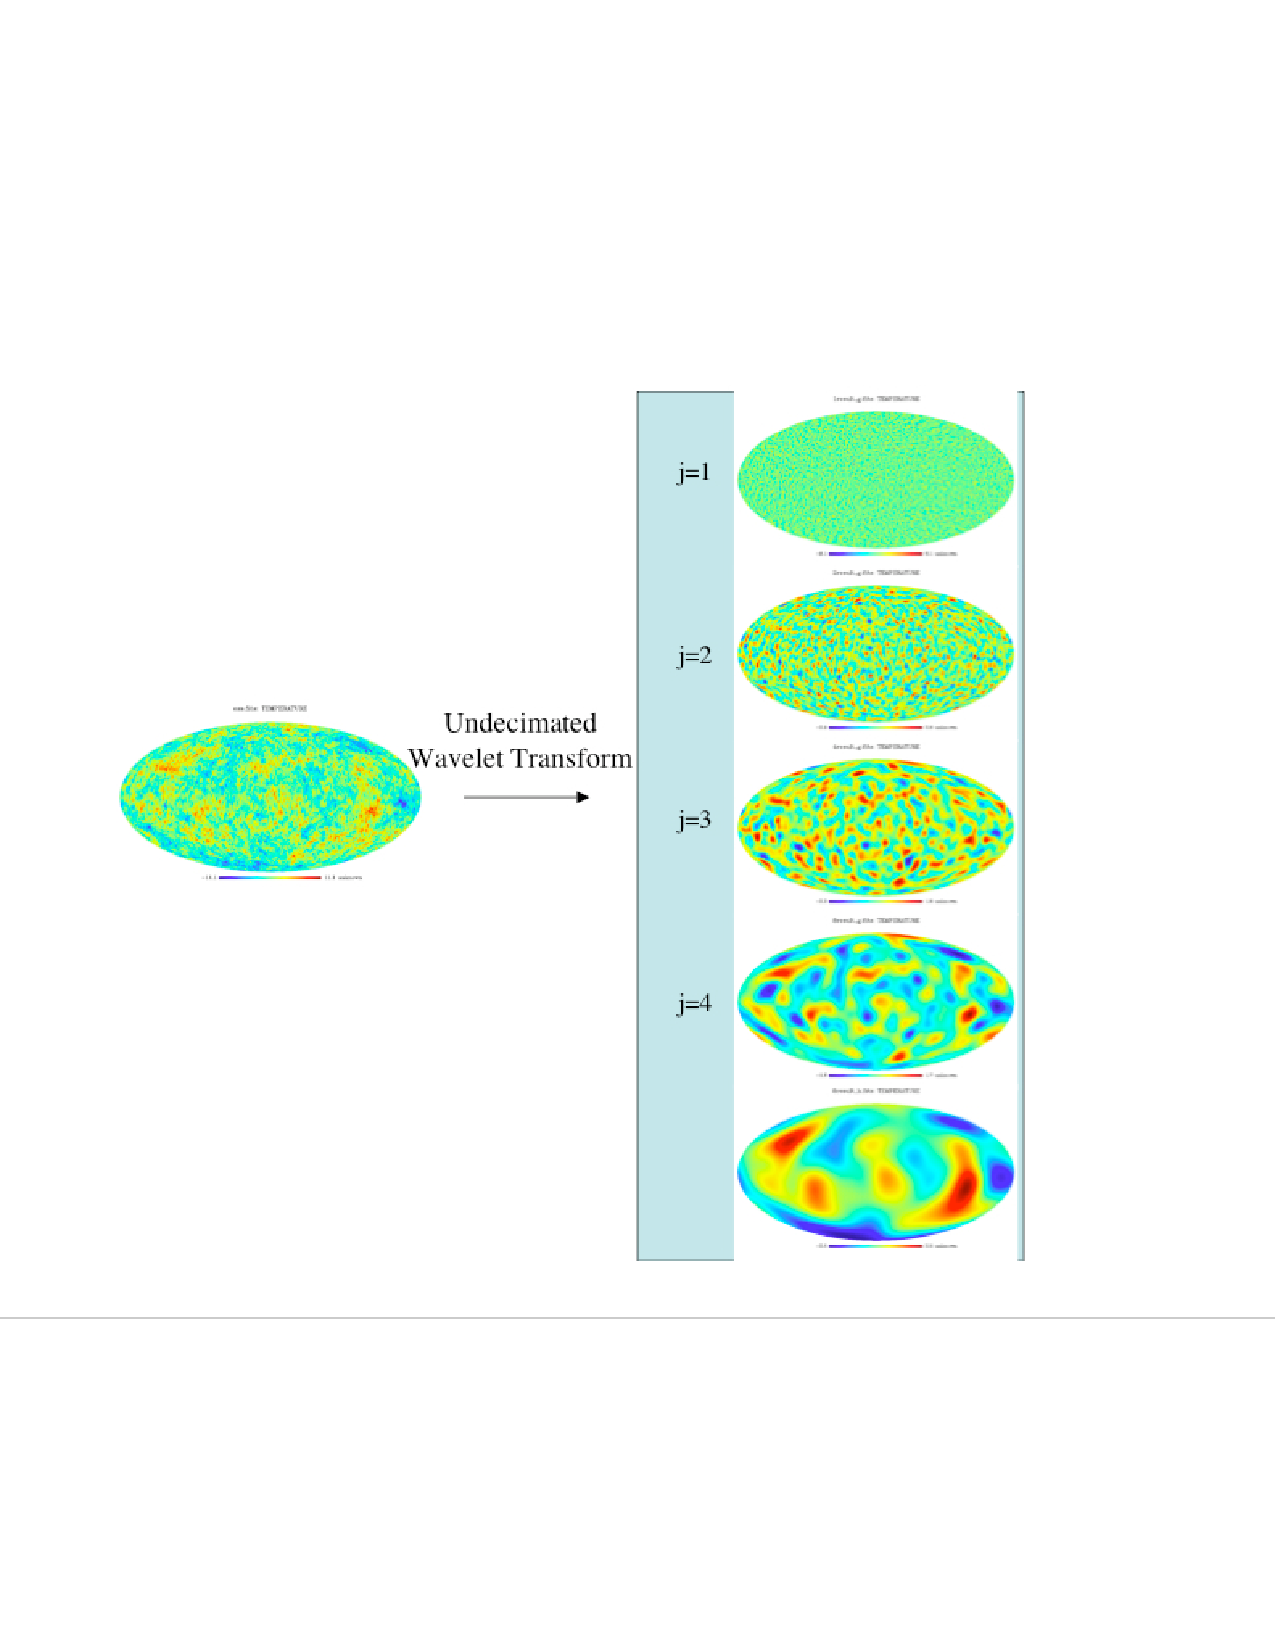
\includegraphics[height=8truecm,width=6truecm]{fig_uwt_sphere.pdf}
% 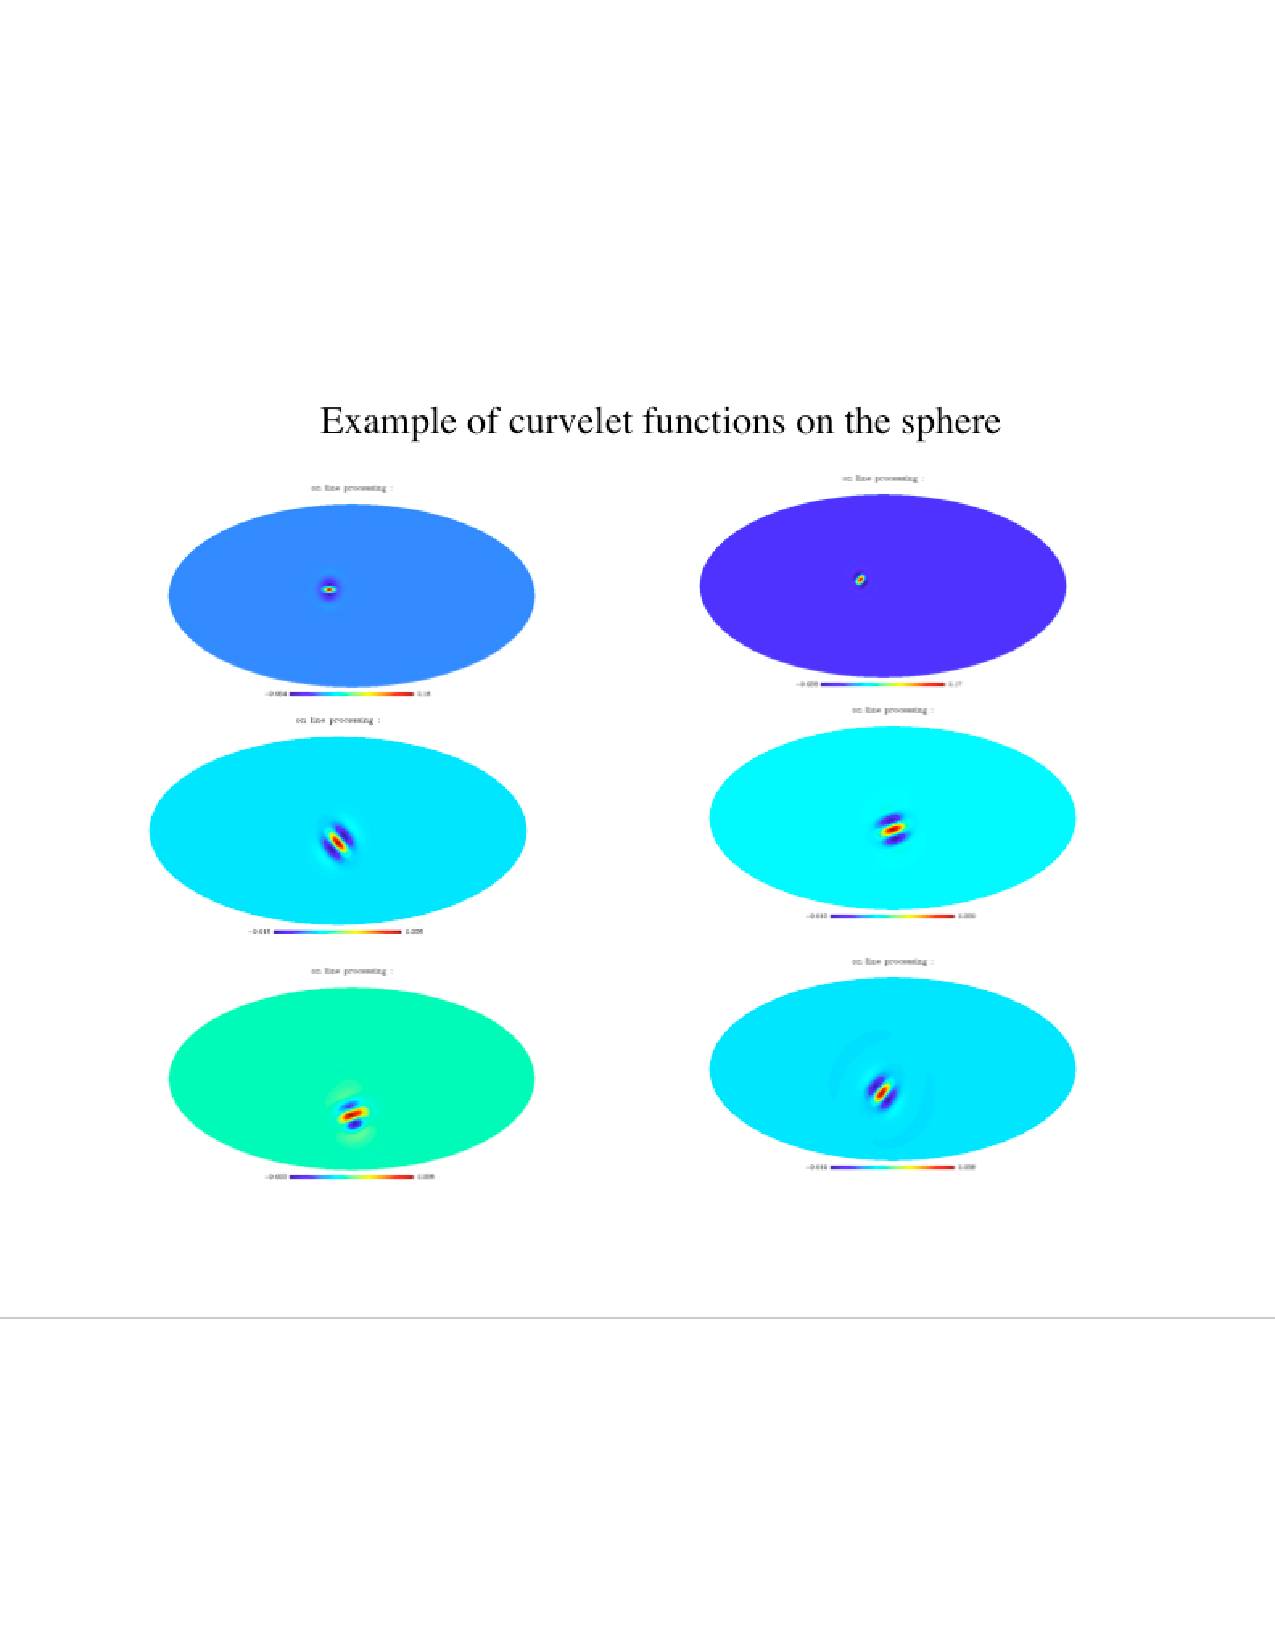
\includegraphics[height = 5 in]{fig_back_cur_sphere.pdf}
\vbox{
\centerline{
\hbox{
\psfig{figure=fig_synchrotron_bw.pdf,bbllx=0.5cm,bblly=9.5cm,bburx=20cm,bbury=20cm,width=8cm,height=4.5cm,clip=}
\psfig{figure=fig_synchrotron_noise5_bw.pdf,bbllx=0.5cm,bblly=9.5cm,bburx=20cm,bbury=20cm,width=8cm,height=4.5cm,clip=}
}}
\centerline{
\hbox{
\psfig{figure=fig_pwt5_synchrotron_noise5_bw.pdf,bbllx=0.5cm,bblly=9.5cm,bburx=20cm,bbury=20cm,width=8cm,height=4.5cm,clip=}
\psfig{figure=fig_resi_pwt5_synchrotron_noise5_bw.pdf,bbllx=0.5cm,bblly=9.5cm,bburx=20cm,bbury=20cm,width=8cm,height=4.5cm,clip=}
}}
\centerline{
\hbox{
\psfig{figure=fig_pcur5_synchrotron_noise5_bw.pdf,bbllx=0.5cm,bblly=9.5cm,bburx=20cm,bbury=20cm,width=8cm,height=4.5cm,clip=}
\psfig{figure=fig_resi_pcur5_synchrotron_noise5_bw.pdf,bbllx=0.5cm,bblly=9.5cm,bburx=20cm,bbury=20cm,width=8cm,height=4.5cm,clip=}
}}
}
\caption{\textbf{Denoising.} Upper left and right : simulated synchrotron image and same image with an additive 
Gaussian noise (\emph{i.e.} simulated data). Middle: pyramidal wavelet filtering and residual. Bottom: pyramidal 
curvelet filtering and residual.{ On such data, presenting very anisotropic features, the residual with a curvelet 
denoising is cleaner than with the wavelet denoising.}}
\label{Figure:sync_filter}
\end{figure*}

Figure~\ref{Figure:sync_filter} describes the setting and the results of a simulated denoising experiment : 
upper left, the original simulated map of the synchrotron emission (renormalized between 0 and 255); upper right, 
the same image plus additive Gaussian noise ($\sigma=5$); middle, the pyramidal wavelet filtered image and the 
residual (i.e. noisy data minus filtered data); bottom, the pyramidal curvelet transform filtered image and the 
residual. A $5 \sigma_j$ detection threshold was used in both cases. On such data, presenting very anisotropic 
features, the curvelets produces better results than the wavelets.


\section{The Combined Filtering Method on the Sphere}
\index{wavelet!combined filtering}
\index{curvelet!combined filtering}
\index{combined filtering method}

%\voffset -1truecm
{\small
\begin{table*}[htb]
\baselineskip=0.4cm
\begin{center}
\begin{tabular}{lccccc} \hline \hline
Method                          &  Error Standard Deviation     &  SNR (dB)    \\ \hline \hline
Noisy map                       & 5.  &      13.65  \\
Wavelet                         & 1.30  &    25.29  \\
Curvelet                        & 1.01  &    27.60  \\
CFM                             & 0.86  &    28.99  \\ \hline
\hline
\end{tabular}
\caption{Table of error standard deviations and SNR values after filtering the synchrotron noisy map (Gaussian white noise - sigma = 5 ) 
by the wavelet, the curvelet and the combined filtering method. Images are available at "http://jstarck.free.fr/mrs.html".}
% \vspace{0.5cm}aa_sphere05
\label{comptab_sync}
\end{center}
\end{table*}
}

\begin{figure}
% 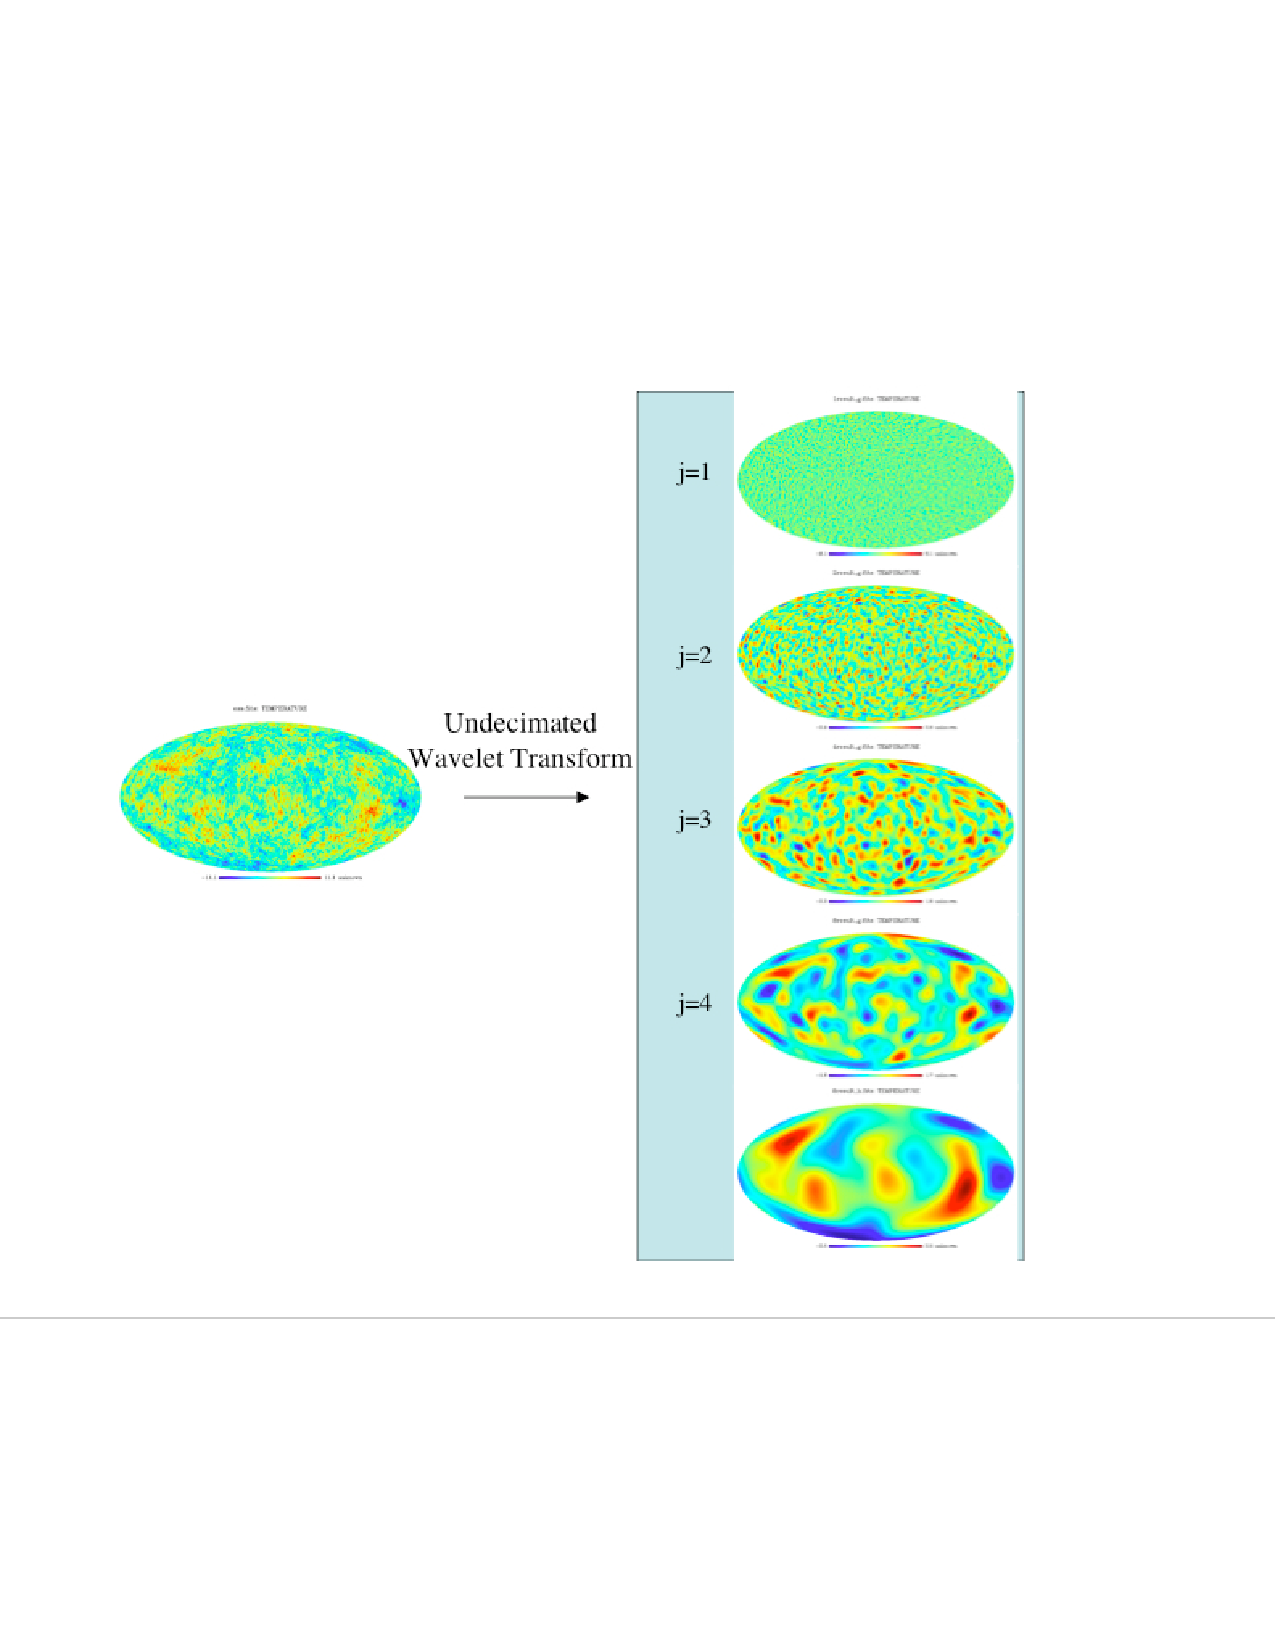
\includegraphics[height=8truecm,width=6truecm]{fig_uwt_sphere.pdf}
% 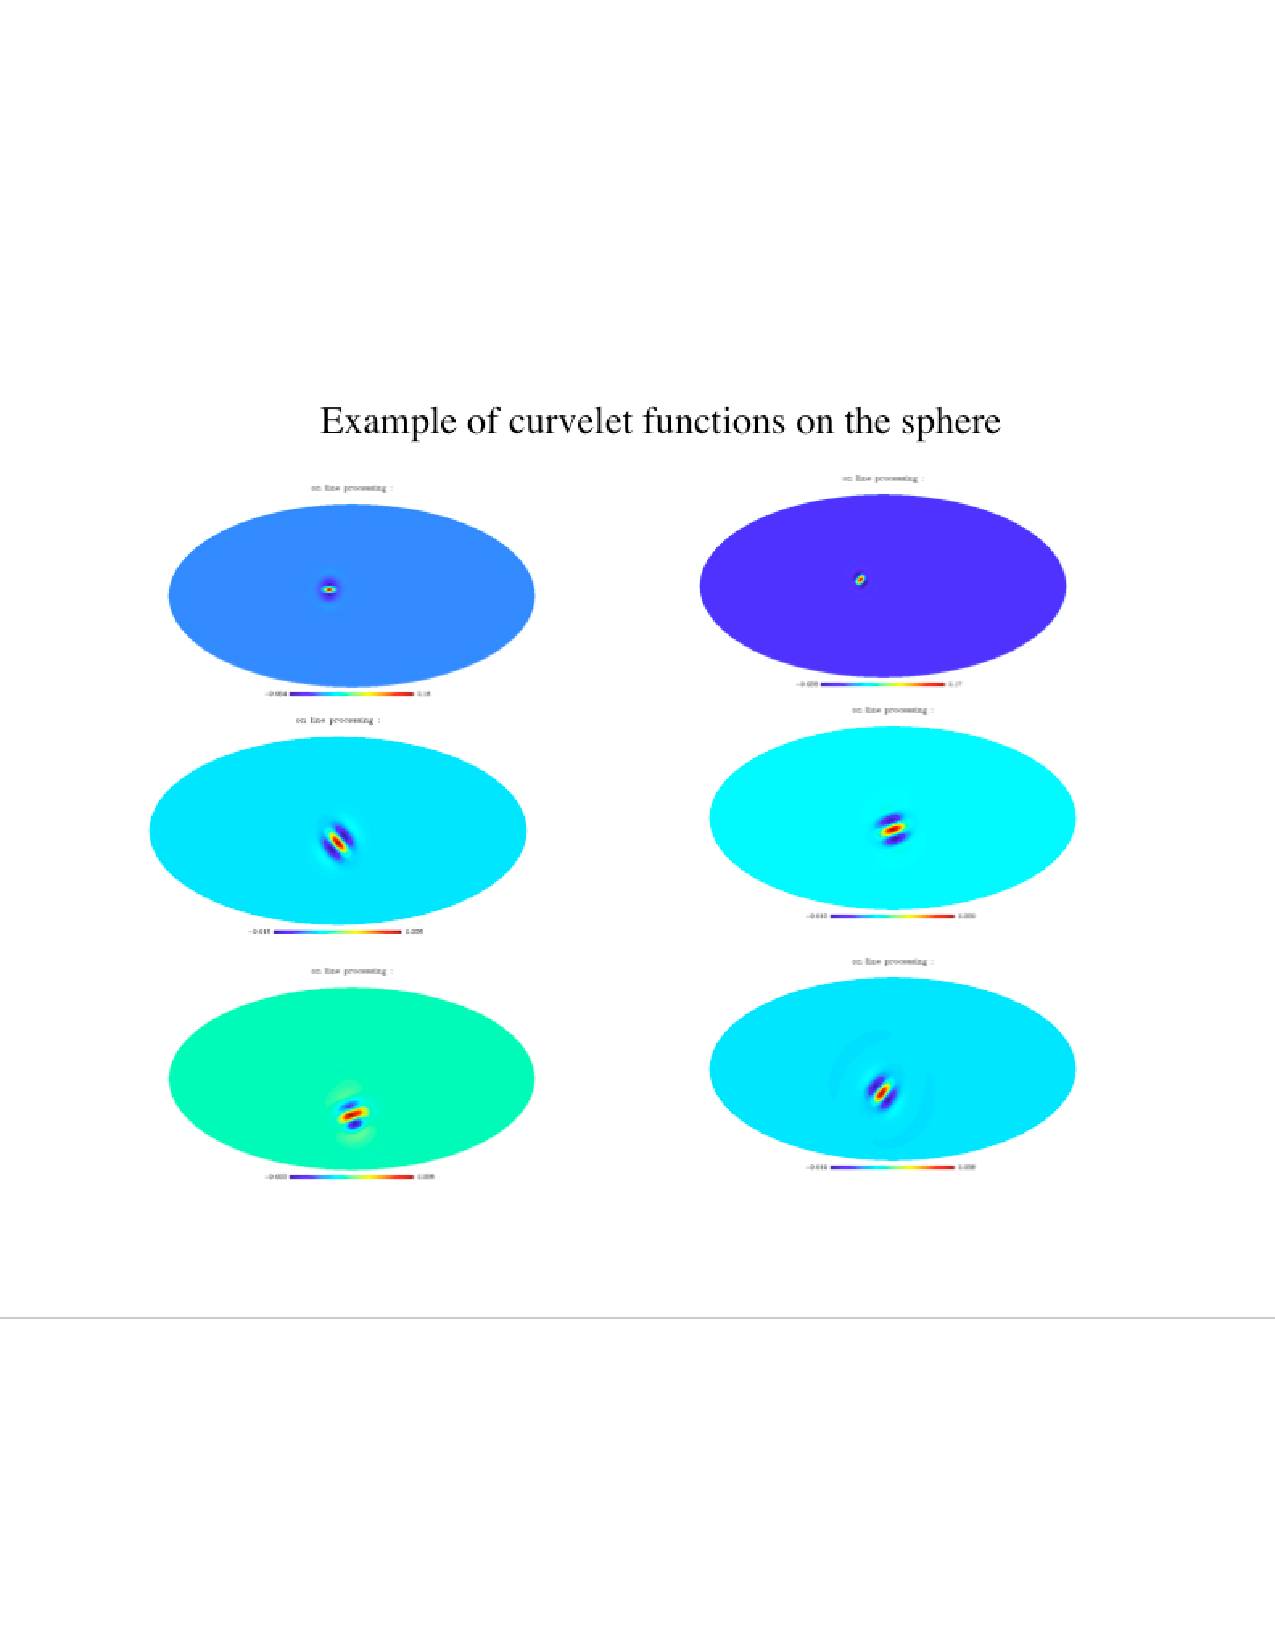
\includegraphics[height = 5 in]{fig_back_cur_sphere.pdf}
\centerline{
\hbox{
\psfig{figure=fig_cbf5_synchrotron_bw.pdf,bbllx=0.5cm,bblly=9.5cm,bburx=20cm,bbury=20cm,width=8cm,height=4.5cm,clip=}
\psfig{figure=fig_resi_cbf5_synchrotron_bw.pdf,bbllx=0.5cm,bblly=9.5cm,bburx=20cm,bbury=20cm,width=8cm,height=4.5cm,clip=}
}}
\caption{Denoising. Combined Filtering Method (pyramidal wavelet and pyramidal curvelet) and residual.}
\label{Figure:sync_cbf_filter}
\end{figure}


\begin{figure}
\centerline{
\hbox{
% \psfig{figure=fig_result_cbf_face5_bw.ps,bbllx=1.5cm,bblly=4.5cm,bburx=20cm,bbury=23cm,height=10cm,width=10cm,clip=}
\psfig{figure=fig_cmp_fil_synchrotron_face6_bw.pdf,bbllx=1.5cm,bblly=12.5cm,bburx=10.5cm,bbury=25.5cm,height=19.5cm,width=13.5cm,clip=}
}}
\caption{{ Combined Filtering Method, face 6 in the Healpix representation of the image shown in figure~\ref{Figure:sync_cbf_filter}. 
From top to bottom and left to right, respectively the a) original image face, b) the noisy image, c) the combined filtered image, 
d) the combined filtering residual, e) the wavelet filtering residual and f) the curvelet filtering residual.}}
\label{Figure:sync_face_cbf_filter}
\end{figure}

Although the results obtained by simply thresholding the curvelet expansion are encouraging, there is of course ample room for further
improvement. A quick inspection of the residual images for both the wavelet and curvelet transforms shown in Figure~\ref{Figure:sync_filter}
reveals the existence of very different features. For instance, wavelets do not restore long features with high fidelity while curvelets
are seriously challenged by isotropic or small features. Each transform has its own area of expertise and this complementarity is of great 
potential. The Combined Filtering Method (CFM) \cite{starck:spie01a} allows us to benefit from the advantages of both transforms. This iterative 
method detects the significant coefficients in both the wavelet domain and the curvelet domain and guarantees that the reconstructed map will 
take into account any pattern which is detected as significant by either of the transforms. A full description of the algorithm is given in Appendix B.
Figure~\ref{Figure:sync_cbf_filter} shows the CFM denoised image and its residual. { Figure~\ref{Figure:sync_face_cbf_filter} shows one face 
(face 6) of the following Healpix images: upper left, original image; upper right, noisy image; middle left, restored image after denoising 
by the combined transform; middle right, the residual; bottom left and right, the residual using respectively the curvelet and the wavelet 
denoising method. } The results are reported in Table~\ref{comptab_sync}. The residual is much better when the combined filtering is applied, 
and no feature can be detected any more by eye in the residual. This was not the case for either the wavelet and the curvelet filtering.

% \section{Deconvolution ?}


\chapter{Statistics on the Sphere and Non-Gaussianities Detection}
\label{ch_fluctu}
\index{statistic}
\section{Introduction}
\index{CMB}
\index{detection!non-Gaussianity}
The search for non-Gaussian signatures in the cosmic microwave background (CMB) temperature fluctuation maps furnished by
MAP\footnote{http://map.gsfc.nasa.gov/} \citep{komatsu2003}, and to be furnished by PLANCK\footnote{http://astro.estec.esa.nl/SA-general/Projects/Planck/},
is of great interest for cosmologists. Indeed, the non-Gaussian signatures in the CMB can be related to very fundamental questions
such as the global topology of the universe \citep{riazuelo2002}, superstring theory, topological defects such as cosmic strings
\citep{gauss:bouchet88}, and multi-field inflation \citep{bernardeau2002}. The non-Gaussian signatures can, however, have a different 
but still cosmological origin. They can be associated with the Sunyaev-Zel'dovich (SZ) effect \citep{sunyaev80} (inverse Compton
effect) of the hot and ionized intra-cluster gas of galaxy clusters \citep{gauss:aghanim99,cooray2001}, with the gravitational 
lensing by large scale structures \citep{threepoint:bernardeau03}, or with the reionization of the universe \citep{gauss:aghanim99,castro2002}. 
They may also be simply due to foreground emission \citep{gauss:jewell01}, or to non-Gaussian instrumental noise and systematics \citep{banday2000}.
\index{SZ effect}
\index{cosmic strings}

All these sources of non-Gaussian signatures might have different origins and thus different statistical and morphological
characteristics. It is therefore not surprising that a large number of studies have recently been devoted to the subject 
of the detection of non-Gaussian signatures. Many approaches have been investigated: Minkowski functionals and the morphological 
statistics \citep{gauss:novikov00,gauss:shandarin02}, the bispectrum (3-point estimator in the Fourier domain) 
\citep{gauss:bromley99,gauss:verde00,gauss:phillips01}, the trispectrum (4-point estimator in the Fourier domain) \citep{gauss:kunz01}, 
wavelet transforms \citep{gauss:aghanim99,gauss:forni99,gauss:hobson99,gauss:barreiro01,gauss:cayon01,gauss:jewell01,starck:sta03_1}, 
and the curvelet transform \citep{starck:sta03_1}. In \citep{gauss:aghanim03,starck:sta03_1}, it was shown that the wavelet transform 
was a very powerful tool to detect the non-Gaussian signatures. Indeed, the excess kurtosis (4th moment) of the wavelet coefficients 
outperformed all the other methods (when the signal is characterized by a non-zero 4th moment). Based on kurtosis of wavelet coefficients, 
recent studies have reported non-Gaussian signatures in the WMAP data \citep{wave:vielva04,gauss:pia04,gauss:cruz05}.
The excess kurtosis is a widely used statistic, based on the 4th moment. 
% For any (symmetrical) random variable $X$, the kurtosis is:
% \[
% \kappa(X) = \frac{EX^4}{(EX^2)^2} -3. 
% \]
The kurtosis measures a kind of departure of $X$ from Gaussianity. The non-Gaussianty detector consists of first applying 
a multiscale transform (e.g., wavelet, or curvelet), and then calculating at each scale the kurtosis. In practice, missing 
data and instrumental effects may create an artificial kurtosis and it is very important to produce realistic simulations 
which present the same caracteristics as the observated data (e.g., missing data, noise, etc.). Then the kurtosis obtained 
from the data is compared to the kurtosis level expected from the simulations.
 
Finally, a major issue of the non-Gaussian studies in CMB remains our ability to disentangle all the sources of non-Gaussianity 
from one another. Recent progress has been made on the discrimination between different possible origins of non-Gaussianity. 
Namely, it was possible to separate the non-Gaussian signatures associated with topological defects (cosmic strings) from those 
due to the Doppler effect of moving clusters of galaxies (both dominated by a Gaussian CMB field) by combining the excess kurtosis 
derived from both the wavelet and the curvelet transforms \citep{starck:sta03_1}. 

The wavelet transform is suited to spherical-like sources of non-Gaussianity, and a curvelet transform is suited to structures 
representing sharp and elongated structures such as cosmic strings. Each provides an adapted non-Gaussian estimator, namely 
the normalised mean excess kurtosis. The combination of these transforms through the product of the normalized mean excess kurtosis 
of wavelet transforms by normalized mean excess kurtosis of curvelet transforms highlights the presence of the cosmic strings 
in a mixture CMB+SZ+CS. Such a combination gives information about the nature of the non-Gaussian signals. The sensitivity of 
each transform to a particular shape makes it a very strong discriminating tool \citep{starck:sta03_1,starck:jin05}.

\begin{figure}[htb]
\centering
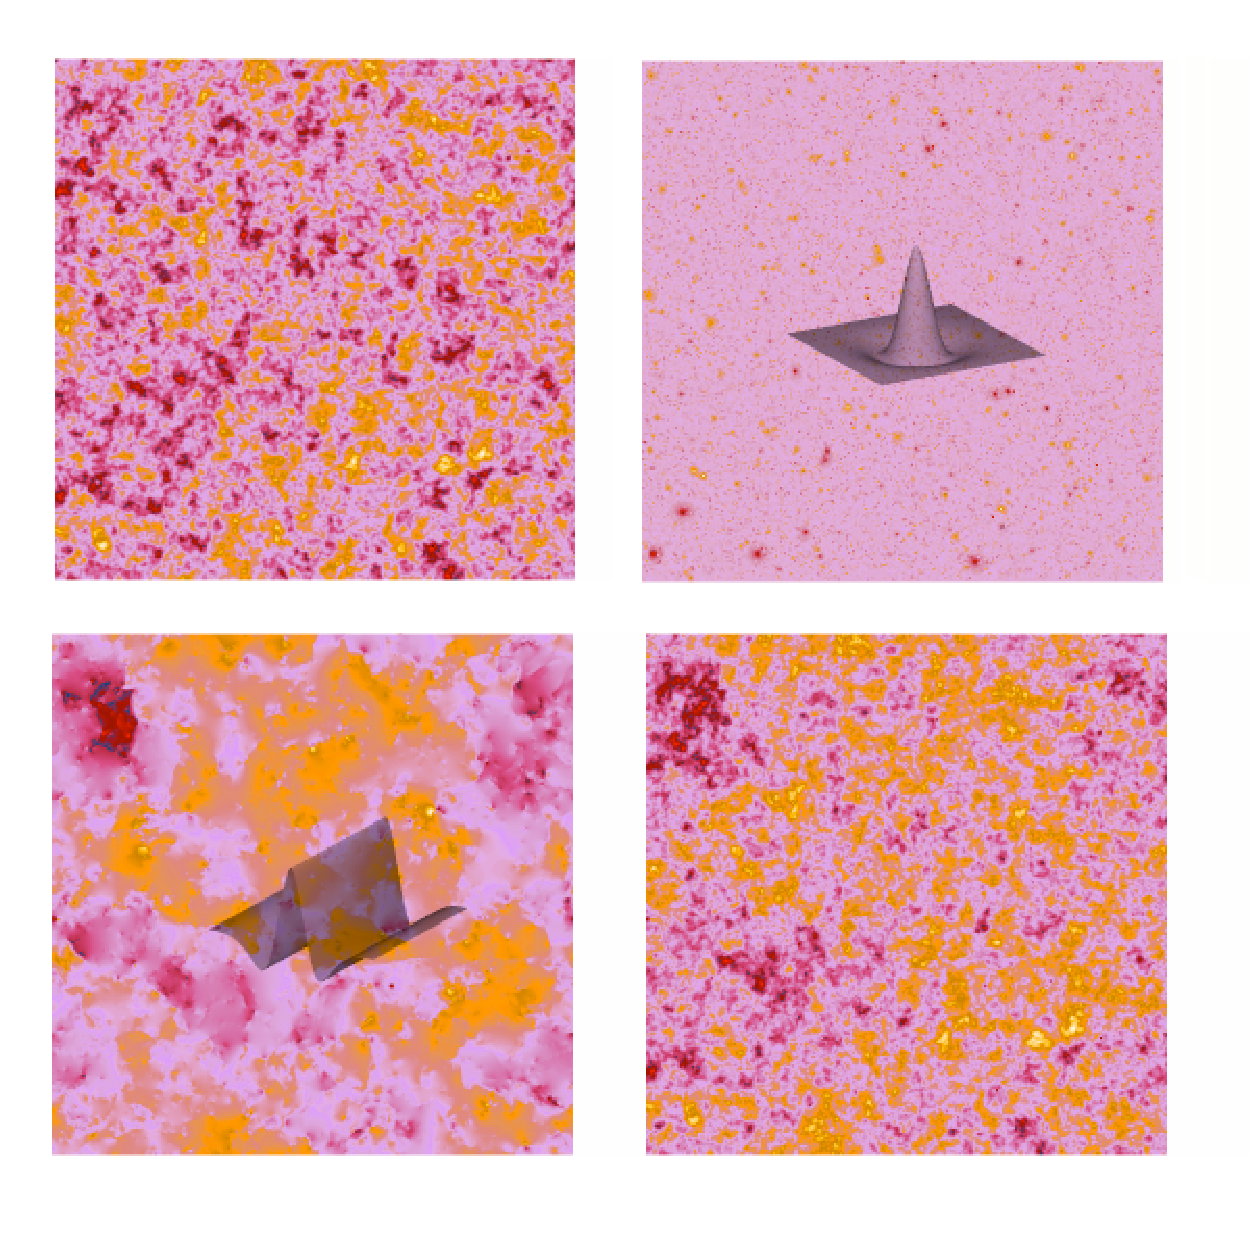
\includegraphics[width=13cm,height=13cm]{fig_cmbcssz.pdf}
\caption{Top, primary Cosmic Microwave Background anisotropies (left) and kinetic Sunyaev-Zel'dovich fluctuations (right). 
Bottom, cosmic string simulated map (left) and simulated observation containing the previous three components (right). 
The wavelet function is overplotted on the Sunyaev-Zel'dovich map and the curvelet function is overplotted on cosmic string map.}
\label{fig_cmb}
\end{figure}

In order to illustrate this, we show in Fig.~\ref{fig_cmb} a set of simulated maps. Primary CMB, kinetic SZ and cosmic string 
maps are shown respectively in Fig.~\ref{fig_cmb} top left, top right and bottom left. The ``simulated observed map", containing 
the three previous components, is displayed in Fig.~\ref{fig_cmb} bottom right. The primary CMB anisotropies dominate all the 
signals except at very high multipoles (very small angular scales). The wavelet function is overplotted on the kinetic Sunyaev-Zel'dovich 
map and the curvelet function is overplotted on cosmic string map.


CMB data are different from other astronomical data sets in the sense that they are not sparse (typical sparse data are stars or/and 
galaxies on top of a smooth background). After a component separation processing (see chapter~\ref{ch_mrs_ica}), the CMB data are not 
completely free of contaminations. Point sources still need to be detected and removed. Once we believe the data are clean enough, 
we want to check if the distribution of CMB temperature fluctuations is Gaussian by using robust statistical Gaussianity tests. 
\index{SZ effect}
\index{cosmic strings}
\index{CMB}

\section{Point Sources on a Gaussian Background}
\index{detection!point sources}
\index{wavelet!mexican hat}
\index{detection!matched filter}

Several methods have been proposed in the last years for point source detection in the CMB such as the the Mexican Hat wavelet \citep{gauss:cayon00,gauss:cayon01}, 
the pseudo-filter \citep{gauss:sanz01}, or the biparametric scale-adaptive filter \citep{gauss:sanz05}. A simple and robust technique, which maximizes 
the signal-to-noise ratio is the Matched Filter \citep{gauss:vio02}. Assuming an isotropic point spread function (PSF) with known power sprectum $\tau(q)$ 
and the CMB with power spectrum $P(q)$, the Matched Filter is \citep{gauss:vio02}:
\begin{equation} 
\label{eqn_mf}
\widehat{\psi}_{MF}(q) = \frac{1}{2 \pi \alpha}~ \frac{\tau(q)}{P(q)},\qquad \alpha \equiv \int_0^{+\infty}q \frac{\tau^2}{P} ~dq
\end{equation}
with minimum variance
\begin{equation} 
\sigma^2 = \frac{1}{2 \pi \alpha}
\end{equation}

\newpage
If the PSF is unknown (or space-variant), the Mexican Hat wavelet may be a good alternative. It consists of convolving the data 
with the wavelet function $\psi_{a,b} (x) =  \psi(\frac{x-b}{a})$, where $\psi(x)= \frac{1}{\sqrt{2\pi}}(1 - x^2) e^{- x^2/2}$. 
$a$ is the scale parameter and $b$ the position parameter. A fast implementation is obtained by using the Fourier transform to 
perform the convolution products ($\widehat{\psi}_{a}(q) = \frac{2}{\sqrt{\pi}} {(q a )}^2 e^{- \frac{1}{2}{(q a)}^2}$) \citep{gauss:sanz05}.




\section{Detecting Faint Non-Gaussian Signals Superposed on a Gaussian Signal}
\label{sec:Theory}
The superposition of a non-Gaussian signal with a Gaussian signal can be modeled as $Y = N + G$, where $Y$ is the observed image, 
$N$ is the non-Gaussian component and $G$ is the Gaussian component. We are interested in using transform coefficients to test 
whether $N \equiv 0$ or not.  

\subsection{Hypothesis Testing and Likelihood Ratio Test (LRT).}  
\label{subsec:LRT}
\index{statistic!LRT}

Transform coefficients of various kinds [Fourier, wavelet, curvelet, etc.] have been used for detecting non-Gaussian behavior 
in numerous studies. Let $X_1, X_2, \ldots, X_n$ be the transform coefficients of $Y$; we model these as  
\begin{equation}    
\label{EqAlt}
X_i = \sqrt{1 - \lam} \cdot  z_i + \sqrt{\lam} \cdot w_i,  \qquad 0< \lam < 1
\end{equation}
where $\lam >0$ is a parameter, $z_i \stackrel{iid}{\sim} N(0,1)$ are the transform coefficients of the Gaussian component $G$, 
$w_i \stackrel{iid}{\sim} W$ are the transform coefficients of the non-Gaussian component $N$, and $W$ is some unknown symmetrical 
distribution. Here without loss of generality, we assume the standard deviation for both $z_i$ and $w_i$ are $1$. 

Phrased in statistical terms, the problem of detecting the existence of a non-Gaussian component is equivalent to discriminating between the hypotheses:  
\begin{eqnarray}
\label{EqHypo2}
&H_0: \;\;\;   X_i = z_i  \label{EqHypo1}   \\
&H_1:   X_i = \sqrt{1 - \lam } \cdot z_i  + \sqrt{\lam} \cdot  w_i,   \qquad 0 < \lam < 1  
\end{eqnarray}
and $N \equiv 0$ is equivalent to $\lam \equiv 0$. We call $H_0$ the {\it null hypothesis $H_0$}, and $H_1$ the {\it alternative hypothesis}. 

% \begin{figure}
% \centering
% \includegraphics[height = 3 in]{PDF/CSDetectRegion.pdf}
% \caption{Detectable regions  in the $\alpha-r$ plane.  With $(\alpha,r)$ in the white region on the top or the undetectable region, all methods completely fail for detection. With $(\alpha,r)$ in the white region on the bottom,  both excess kurtosis and Max/HC are able to detect reliably.      While in the blue region to the left,  Max/HC is able to detect reliably, but excess kurtosis completely fails, and in the yellow region to the right, excess kurtosis is able to detect reliably, but Max/HC  completely fail.     }
% \label{Figure:Detect}
% \end{figure}

\begin{figure}[htb]
\centerline{
\hbox{
\includegraphics[width=12cm]{CSDetectRegion.pdf}%,height=12cm
% \psfig{figure=,bbllx=1.5cm,bblly=8.cm,bburx=19.5cm,bbury=23cm,height=6cm,width=7.5cm,clip=}
 }}
\caption{Detection Boundary in the $\alpha-r$ plane. The solid curve is the detection boundary of LRT, above which is not possible to detect, 
and below which it is possible to reliably detect, the dotted line segment and solid line segment together is the detection boundary for Kurtosis, 
the dotted curve and the solid curve together is the detection boundary of Max/HC. Right panel: detectable regions for Kurtosis, Max/HC.}
\label{Figure:Detect}
\end{figure}

When both $W$ and $\lam$ are known, then the optimal test for Problem (\ref{EqHypo1}) - (\ref{EqHypo2}) is simply 
the Neyman-Pearson Likelihood ratio test (LRT), \cite[Page 74 ]{Lehmann}. The size of $\lam = \lam_n$  for which 
reliable discrimination between $H_0$ and $H_1$ is possible can be derived using asymptotics. If we assume that 
the tail probability of $W$ decays algebraically, 
\begin{equation} \label{EqDefineAlg}
\lim_{x \goto \infty}   x^{\alpha}  P\{|W| > x\}  = C_{\alpha},  \qquad \mbox{$C_{\alpha}$ is a constant}
\end{equation}
(we say $W$ has a power-law tail), and we calibrate $\lam$ to decay with $n$, so that increasing amounts of data are offset by increasingly hard challenges: 
\begin{equation}   \label{EqDefineLam}
\lam = \lam_n  = n^{-r}  
\end{equation}
then there is a {\it threshold effect} for the detection problem (\ref{EqHypo1}) - (\ref{EqHypo2}). In fact, define:\\
\begin{equation} \label{EqDetectBoundary}
\rho^*_1(\alpha) = 
\left\{ \begin{array}{ll}
2/\alpha, &\   \  \alpha \leq 8 \\
1/4, &\     \       \alpha > 8
\end{array}
\right.
\end{equation}
then as $n \goto \infty$, LRT is able to reliably detect for large $n$ when $r < \rho^*_1(\alpha)$, and is unable to detect 
when $r > \rho^*_1(\alpha)$; this is proved in \citep{DJ04b}. Since LRT is optimal, it is not possible for any statistic to 
reliably detect when $r > \rho^*_1(\alpha)$. We call the curve $r = \rho^*_1(\alpha)$ in the $\alpha$-$r$ plane the 
{\it detection boundary}; see Figure \ref{Figure:Detect}.\\

In fact, when $r < 1/4$, asymptotically LRT is able to reliably detect whenever $W$ has a finite $8$-th moment, even without 
the assumption that $W$ has a power-law tail. Of course, the case that $W$ has an infinite $8$-th moment is more complicated, 
but if $W$ has a power-law tail, then LRT is also able to reliably detect if $r < 2/\alpha$. 

% One component of the above result is that, by assuming  $W$ has an 
% $\alpha$-algebraic tail 
% with $\alpha > 8$, then when $r < \frac{1}{4}$,  LRT is 
% able to reliably detect;  
% and when $r > \frac{1}{4}$, no statistic is able to detect.  
% It is interesting to notice here that, this part of the conclusion will still hold 
% when  
% the condition of requiring $W$ to have an algebraic tail is largely relaxed:  in 
% fact,  the same conclusion still holds if we only require $E[W^8] < \infty$.  It is 
% interesting to notice here that,  when $W$ has an $\alpha$-algebraic tail, 
% $E[W^8] < \infty$ if and only if $\alpha > 8$.

Despite its optimality, LRT is not a practical procedure. To apply LRT, one needs to specify the value of $\lam$ and 
the distribution of $W$, which seems unlikely to be available. We need non-parametric detectors, which can be implemented 
without any knowledge of $\lam$ or $W$, and depend on $X_i$'s only. In the next section, we are going to introduce three 
non-parametric detectors: excess kurtosis, Max and Higher Criticism (HC).   

\section{Kurtosis, HC from Wavelet and Curvelet Coefficients}
 
\subsection{Kurtosis}
\index{statistic!Kurtosis}
\index{Kurtosis}

For a statistic $T_n$, the $p$-value is the probability of seeing equally extreme results under the null hypothesis:
\[
p = P_{H_0} \{ T_n  \geq t_n(X_1,X_2, \ldots,X_n) \}
\] 
here $P_{H_0}$ refers to probability under $H_0$, and $t_n(X_1,X_2, \ldots,X_n)$ is the observed value of statistic $T_n$. 
Notice that the smaller the $p$-value, the stronger the evidence against the null hypothesis. A natural decision rule based 
on $p$-values rejects the null when $p < \alpha$ for some selected level $\alpha$, and a convenient choice is  $\alpha = 5\%$. 
When the null hypothesis is indeed true, the $p$-values for any statistic are distributed as uniform $U(0,1)$. This implies 
that the $p$-values provide a common scale for comparing different statistics. 

We now introduce two statistics for comparison. 

{\bf Excess Kurtosis ($\kappa_n$)}. Excess kurtosis is a widely used statistic, based on the $4$-th moment. 
For any (symmetrical) random variable $X$, the kurtosis is:
\[
\kappa(X) = \frac{EX^4}{(EX^2)^2} -3
\]
The kurtosis measures a kind of departure of $X$ from  Gaussianity, as $\kappa(z) =  0$.
Empirically, given $n$ realizations of $X$, the excess kurtosis statistic is defined as: 
\begin{equation}  \label{EqDefineK}
\kappa_n(X_1, X_2,\ldots,X_n)  = \sqrt{\frac{n}{24}} \biggl[ \frac{\frac{1}{n}\sum_i  X_i^4}{(\frac{1}{n}  \sum_i X_i^2)^2}  - 3  \biggr]
\end{equation} 
When the null is true, the excess kurtosis statistic is asymptotically normal:
\[
\kappa_n(X_1, X_2,\ldots,X_n)  \rightarrow_{w}  N(0,1), \qquad n \goto \infty
\]
thus for large $n$, the $p$-value of the excess kurtosis is approximately:
\[
\tilde{p} = \bar{\Phi}^{-1} (\kappa_n(X_1, X_2,\ldots,X_n))
\]
where $\bar{\Phi}(\cdot)$ is the survival function (upper tail probability) of $N(0,1)$. 

It is proved in \citep{DJ04b} that the excess kurtosis is asymptotically optimal for the hypothesis testing of \eqref{EqHypo1} - \eqref{EqHypo2} if 
\[
E [W^8] < \infty
\]
However, when $E[W^8] = \infty$, even though kurtosis is well-defined ($E[W^4] < \infty$), there are situations in which LRT 
is able to reliably detect but excess kurtosis completely fails. In fact, by assuming \eqref{EqDefineAlg} - \eqref{EqDefineLam} 
with an $\alpha < 8$, if $(\alpha,r)$ falls into the blue region of Figure~\ref{Figure:Detect}, then LRT is able to reliably detect, 
however, excess kurtosis completely fails. This shows that in such cases, excess kurtosis is not optimal; see \citep{DJ04b}. 

\subsection{Max}
\index{statistic!max}
\index{max}
The largest (absolute) observation is a classical and frequently-used non-parametric statistic:
\[
M_n =  \mmax(|X_1|,|X_2|,\ldots, |X_n|)
\] 
under the null hypothesis, 
\[
M_n  \approx \sqrt{2 \log n}
\]
and moreover, by normalizing $M_n$ with constants $c_n$ and $d_n$, the resulting statistic 
converges to the Gumbel distribution $E_v$, whose cdf is $e^{-e^{-x}}$:
\[
\frac{M_n - c_n}{d_n}  \rightarrow_{w}    E_v
\]
where approximately
\[
d_n = \frac{\sqrt{6} S_n}{\pi}, \qquad  c_n = \bar{X} - 0.5772 d_n 
\]
here $\bar{X}$ and $S_n$ are the sample mean and sample standard deviation of $\{X_i\}_{i=1}^n$ respectively. 
Thus a good approximation of the $p$-value for $M_n$ is:
\[
\tilde{p} =  \mathrm{exp}(-\mathrm{exp}(-\frac{M_n - c_n}{d_n}))
\]
We have tried the above experiment for $n = 244^2$, and found that taking $c_n = 4.2627$, $d_n = 0.2125$ gives a good approximation.  

Assuming \eqref{EqDefineAlg} - \eqref{EqDefineLam} and $\alpha < 8$, or $\lam = n^{-r}$ and that $W$ has a power-law tail 
with $\alpha < 8$, it is proved in \citep{DJ04b} that Max is optimal for hypothesis testing \eqref{EqHypo1} - \eqref{EqHypo2}. 
Recall if we further assume $\frac{1}{4} < r < \frac{2}{\alpha}$, then asymptotically, excess kurtosis completely fails; 
however, Max is able to reliably detect and is competitive to LRT. 

On the other hand, recall that excess kurtosis is optimal for the case $\alpha > 8$. In comparison, in this case, 
Max is not optimal. In fact, if we further assume $ \frac{2}{\alpha} < r < \frac{1}{4}$, then  excess kurtosis 
is able to reliably detect, but Max will completely fail. 

In Figure \ref{Figure:Detect}, we compared the detectable regions of the excess kurtosis and Max in the $\alpha$-$r$ plane. 

\subsection{Higher Criticism}
\label{sec:HC}
\index{statistic!Higher Criticism}
\index{Higher Criticism}

The Higher Criticism statistic (HC), was proposed in \citep{gauss:lin02}. To define HC first we convert the individual $X_i$'s 
into $p$-values for individual $z$-tests. Let $p_i = P\{ N(0,1) > X_i \}$ be the $i^{th}$ $p$-value, and let $p_{(i)}$ denote 
the $p$-values {\it sorted in increasing order}; the Higher Criticism statistic is defined as:
\[
       HC_{n}^* =  \max_{i}
         \biggl| \sqrt{n} [i/n  - p_{(i)}]/ \sqrt{p_{(i)} (1-p_{(i)})} \biggr|
\]
or in a modified form:
\[
HC_n^+  = \max_{\{i:  \; 1/n  \leq  p_{(i)} \leq  1 - 1/n \}}
         \biggl|   \sqrt{n} [i/n  - p_{(i)}]/ \sqrt{p_{(i)} (1-p_{(i)})}  \biggr|
\]
we let $HC_n$ refer either to $HC_n^*$ or $HC_n^+$ whenever there is no confusion. The above definition is slightly 
different from \citep{gauss:lin02}, but the ideas are essentially the same.

With an appropriate normalization sequence:
\[
a_n = \sqrt{2 \log \log n}, \qquad b_n = 2 \log \log n + 0.5 \log \log \log n - 0.5 \log (4 \pi)
\]
the distribution of $HC_n$ converges to  the Gumbel distribution $E_v^4$, whose cdf is $\mathrm{exp}(-4\mathrm{exp}(-x))$, \citep{Shorack}:
\[
a_n  HC_n - b_n  \rightarrow_w  E_v^4
\]
so the $p$-values of $HC_n$ are approximately:
\begin{equation}  
\label{EqHCP}
\mathrm{exp}(-4\mathrm{exp}( - [a_n HC_n - b_n]))
\end{equation}
For moderately large $n$, in general, the approximation in \eqref{EqHCP} is accurate for the $HC_n^+$, but not for $HC_n^*$.   

A brief remark comparing Max and HC. Max only takes into account the few largest observations, HC takes into account those outliers, 
but also moderate large observations. As a result, in general HC is better than Max, especially when we have unusually many moderately 
large observations. However, when the actual evidence lies in the middle of the distribution both HC and Max will be very weak.

% \section{The Genus and the Multiscale Genus}

\section{Experiments}

\begin{figure}[htb]
\vbox{
\centerline{
\hbox{
 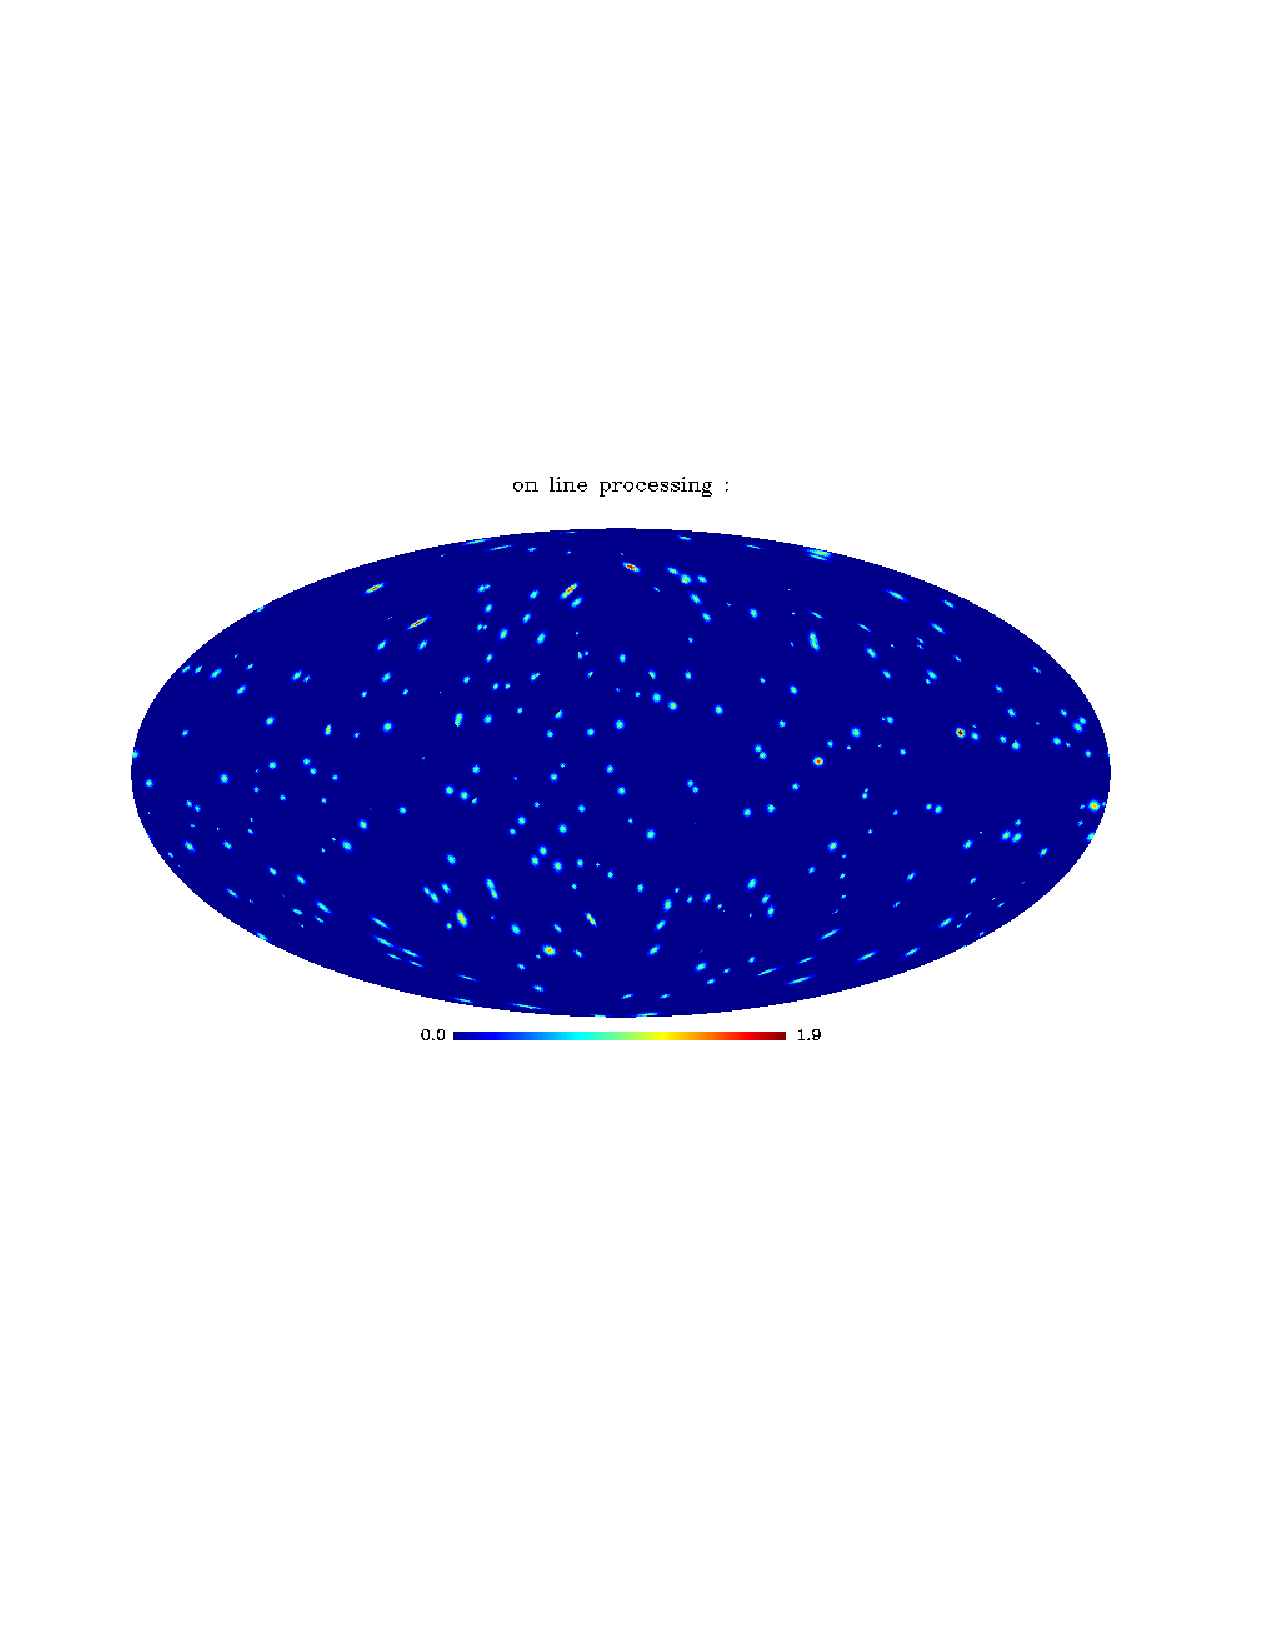
\includegraphics[trim= 2cm 8cm 2cm 8cm,width=7.9cm]{fig_sphere_gaussian.pdf}%[width=8.5cm,height=4.5cm]
 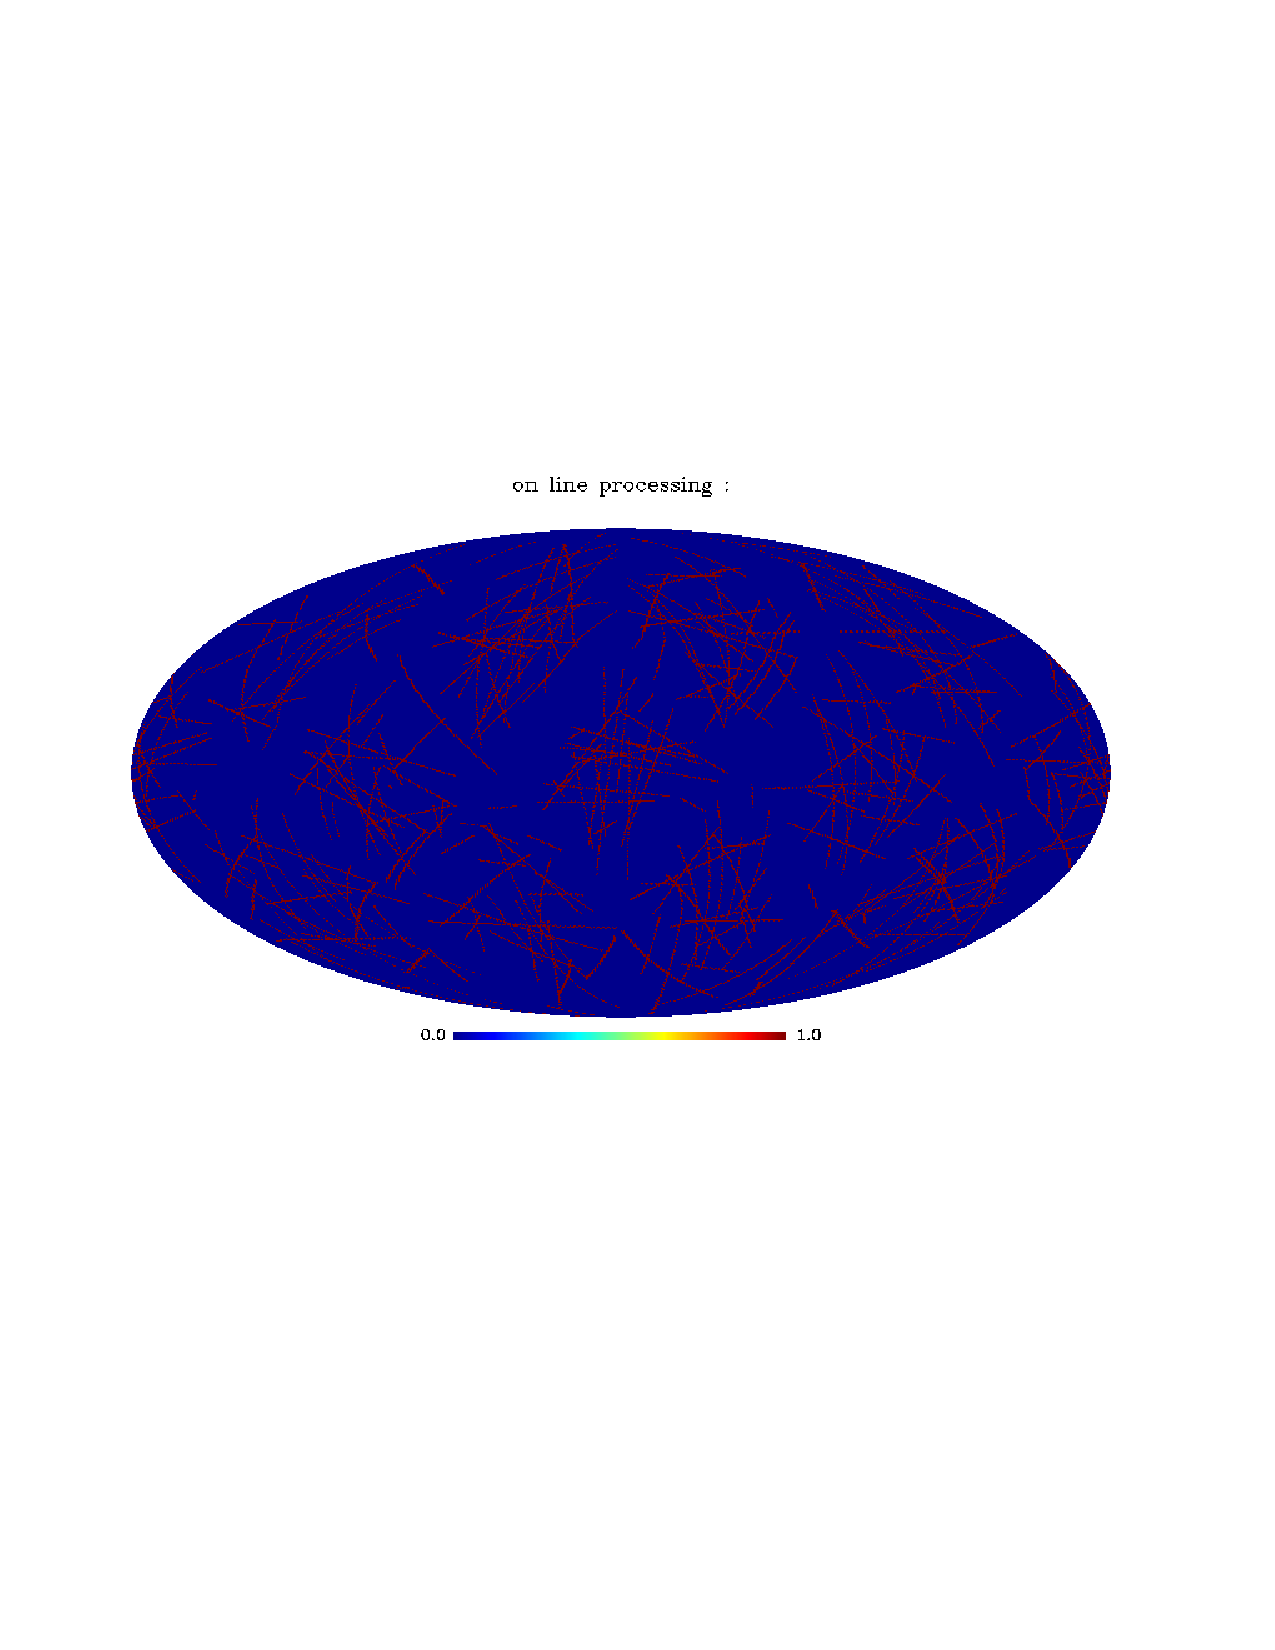
\includegraphics[trim= 2cm 8cm 2cm 8cm,width=7.9cm]{fig_sphere_line.pdf}
}}
 \centerline{
 \hbox{
 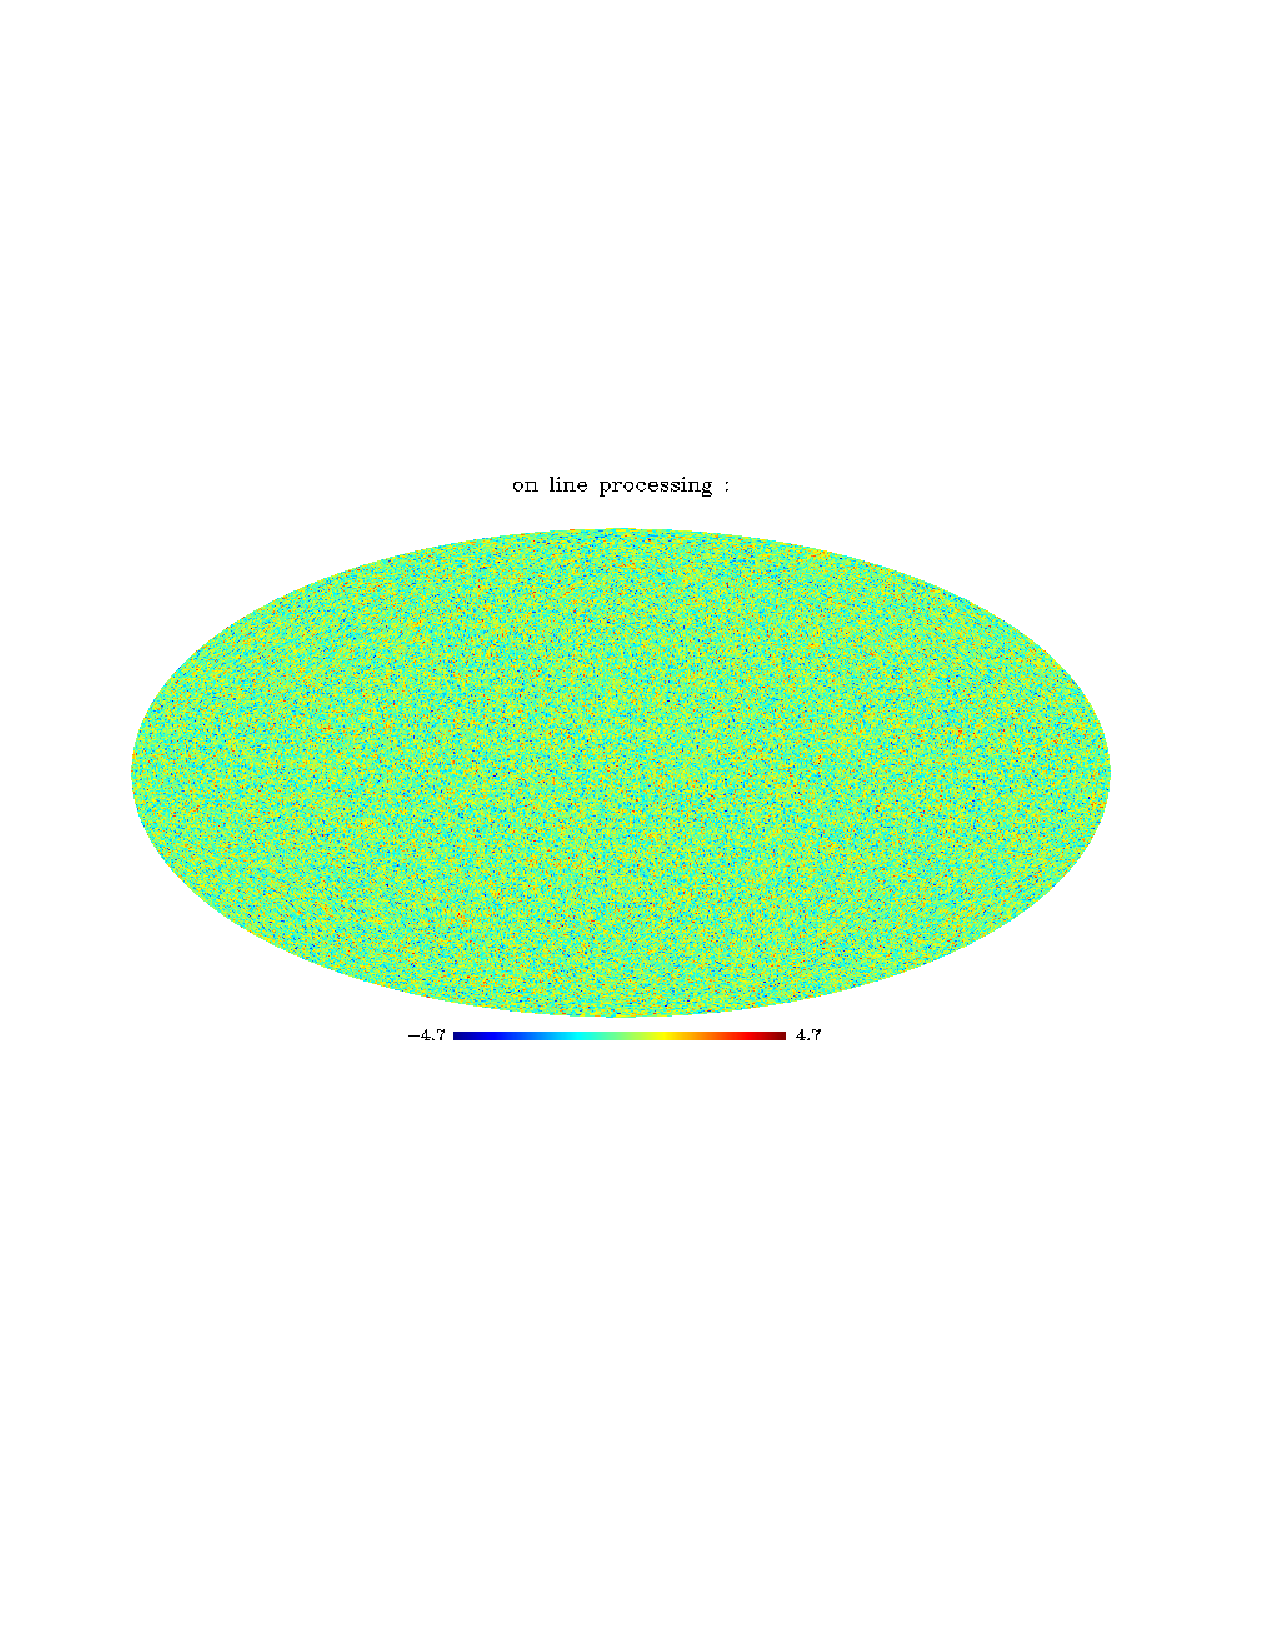
\includegraphics[trim= 2cm 8cm 2cm 8cm,width=7.9cm]{fig_sphere_gaussian_noise_snr1.pdf}
 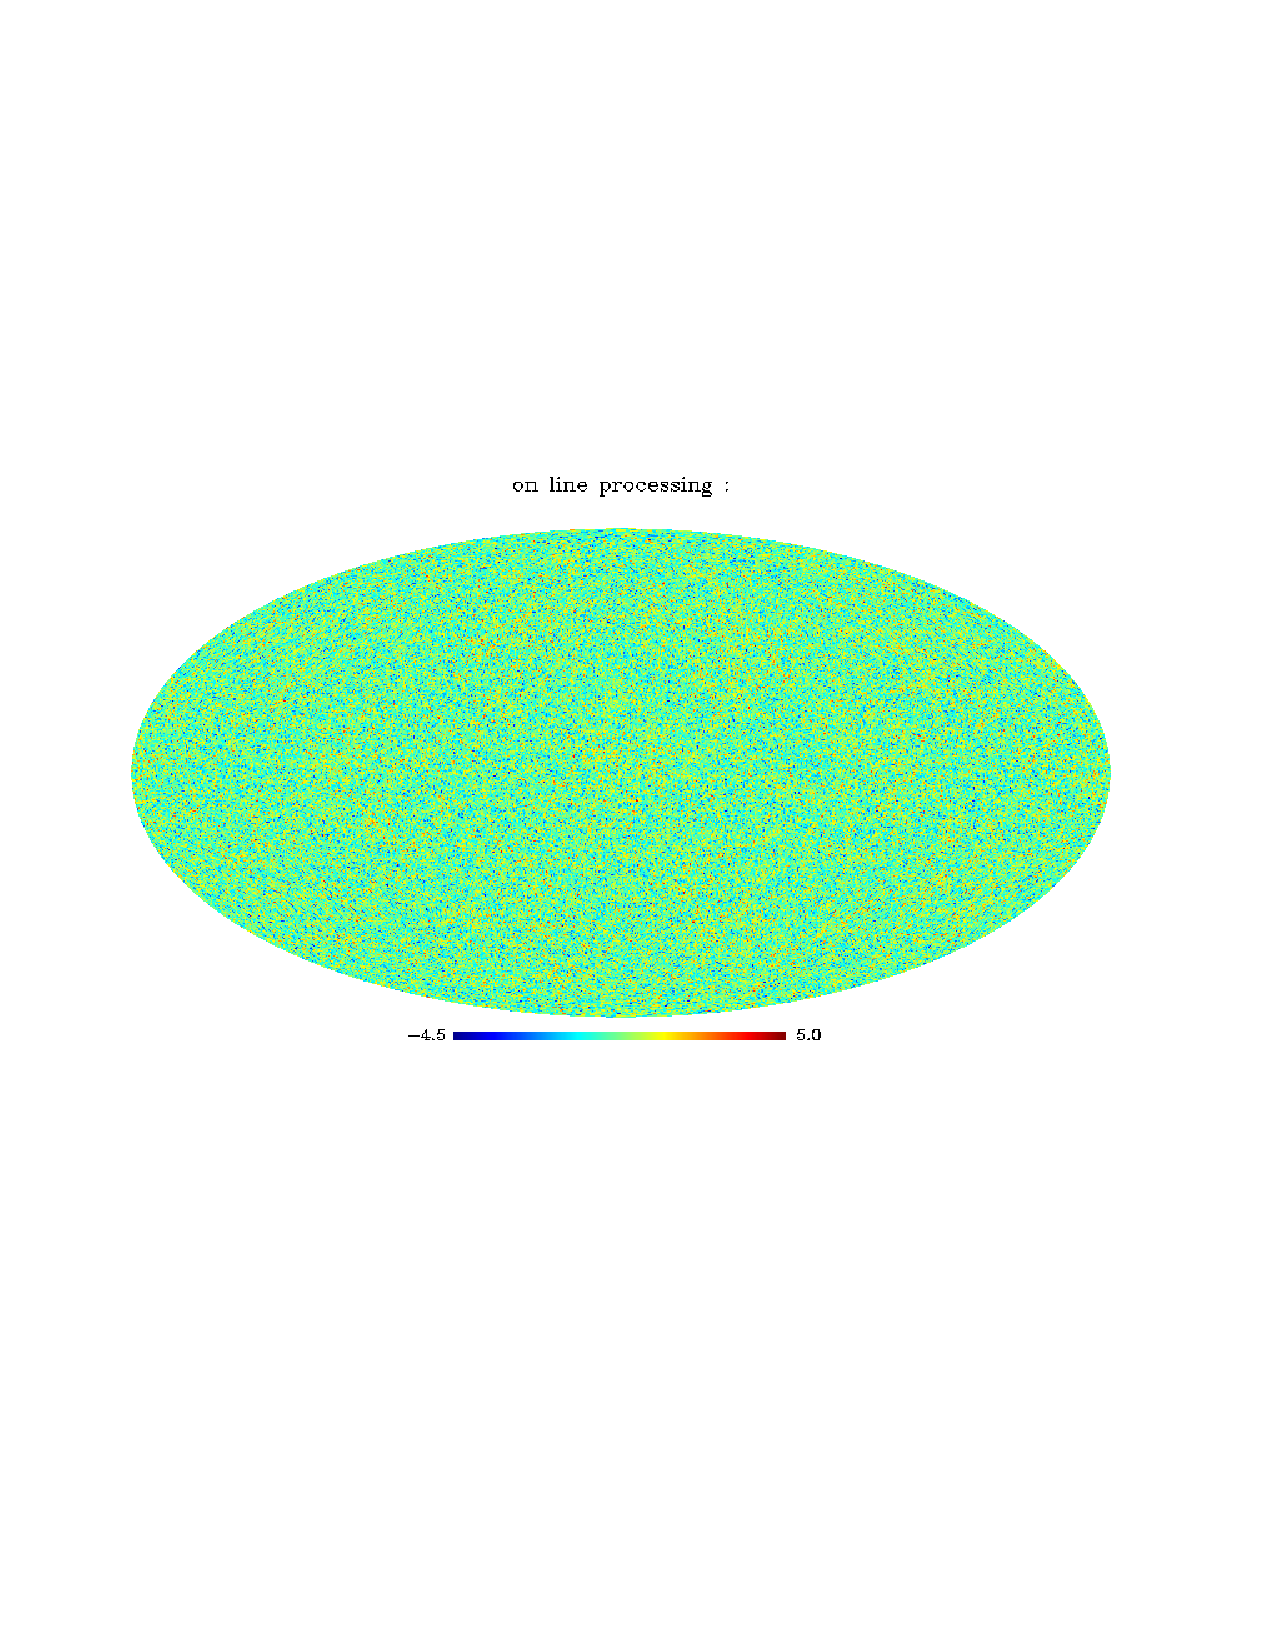
\includegraphics[trim= 2cm 8cm 2cm 8cm,width=7.9cm]{fig_sphere_line_noise_snr1.pdf}
}}}
 \caption{Top, image with Gaussians and image with lines. Bottom, same images but with an additional Gaussian noise. The SNR is equal to 1.}
\label{fig_sphere_linegauss}
\end{figure}

Fig.~\ref{fig_sphere_linegauss} shows, top left and right, two images with respectively Gaussians and lines. We have created a set 
of simulated images by adding a Gaussian white noise with different standard deviations to these two images. The Signal to Noise 
Ratio (SNR) varies between 0 and 1. For the image with lines, the SNR is defined as the pixel values along the lines divided by the 
noise standard deviation, and  for the image with Gaussians, the SNR is defined as the maximum of the Gaussians divided by the noise 
standard deviation. Fig.~\ref{fig_sphere_linegauss} shows, bottom left and right, the two noisy images with a SNR equal to 1. Hence, 
for each SNR value, we have thirty realizations of the noise, and we have calculated the kurtosis at the different scales of both the 
curvelet and the wavelet coefficients. These kurtosis values were normalized by the standard deviation of the kurtosis obtained from 
the wavelet and the curvelet transform of thirty Gaussian white noise realizations. Finally we kept for each SNR the maximum normalized 
kurtosis along the scales. Fig.~\ref{fig_wtcur_sphere_linegauss} left (resp.~right) shows the normalized kurtosis values using the wavelet 
transform (resp. the curvelet transform) for the two images (i.e. lines and Gaussians) versus the SNR. Continuous error bars correspond 
to $1\sigma$ level and dashed error bars correspond to $2\sigma$ level. We can clearly see that the detection power of the wavevet 
transform is much larger than the detection power of the curvelet transform for detecting non-Gaussianities due to isotropic features, 
while curvelets are more powerful than wavelets for detecting anisotropic features.

\begin{figure}[htb]
\centerline{
 \hbox{
% {figure=,bbllx=2.5cm,bblly=12.5cm,bburx=19.5cm,bbury=25.5cm,width=8.5cm,height=6.5cm,clip=}
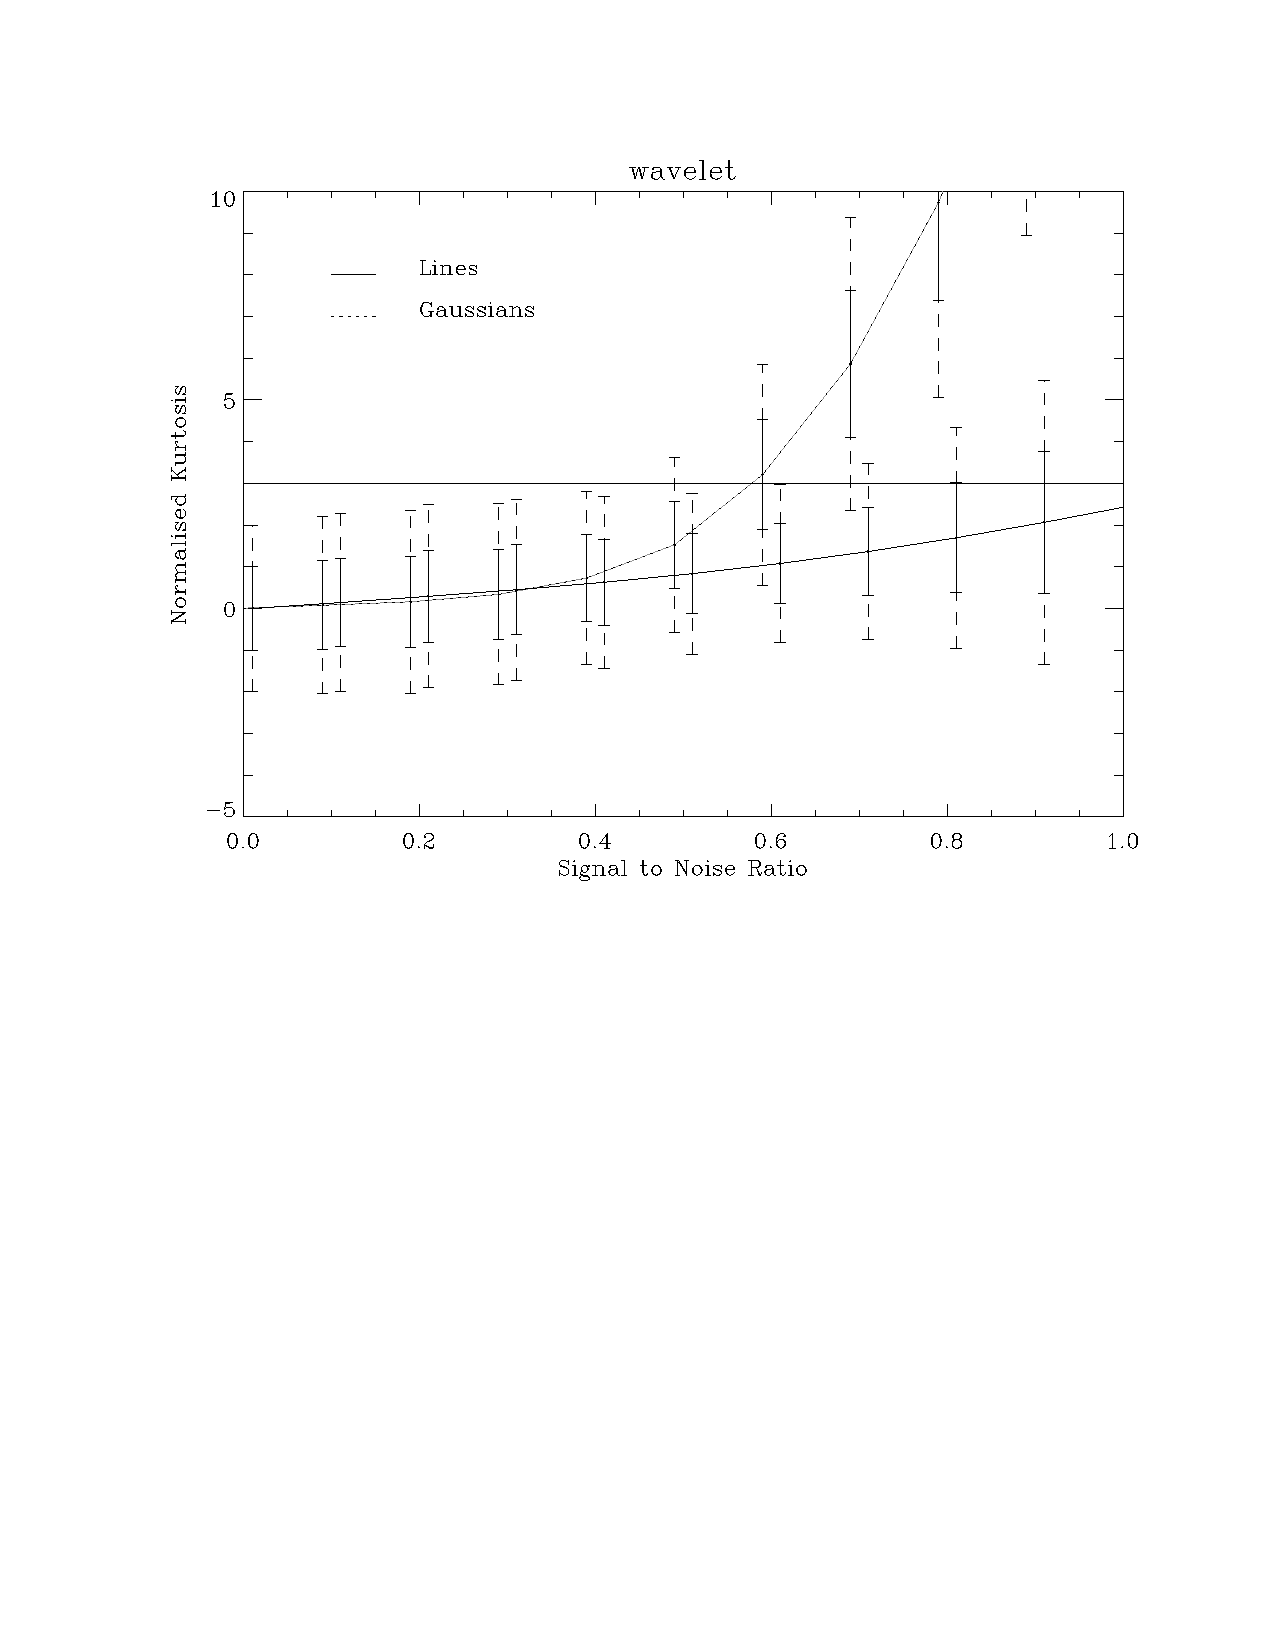
\includegraphics[trim= 2cm 13cm 2cm 3cm,width=7.9cm]{fig_sphere_wt_linedroite.pdf}%,height=6.5cm
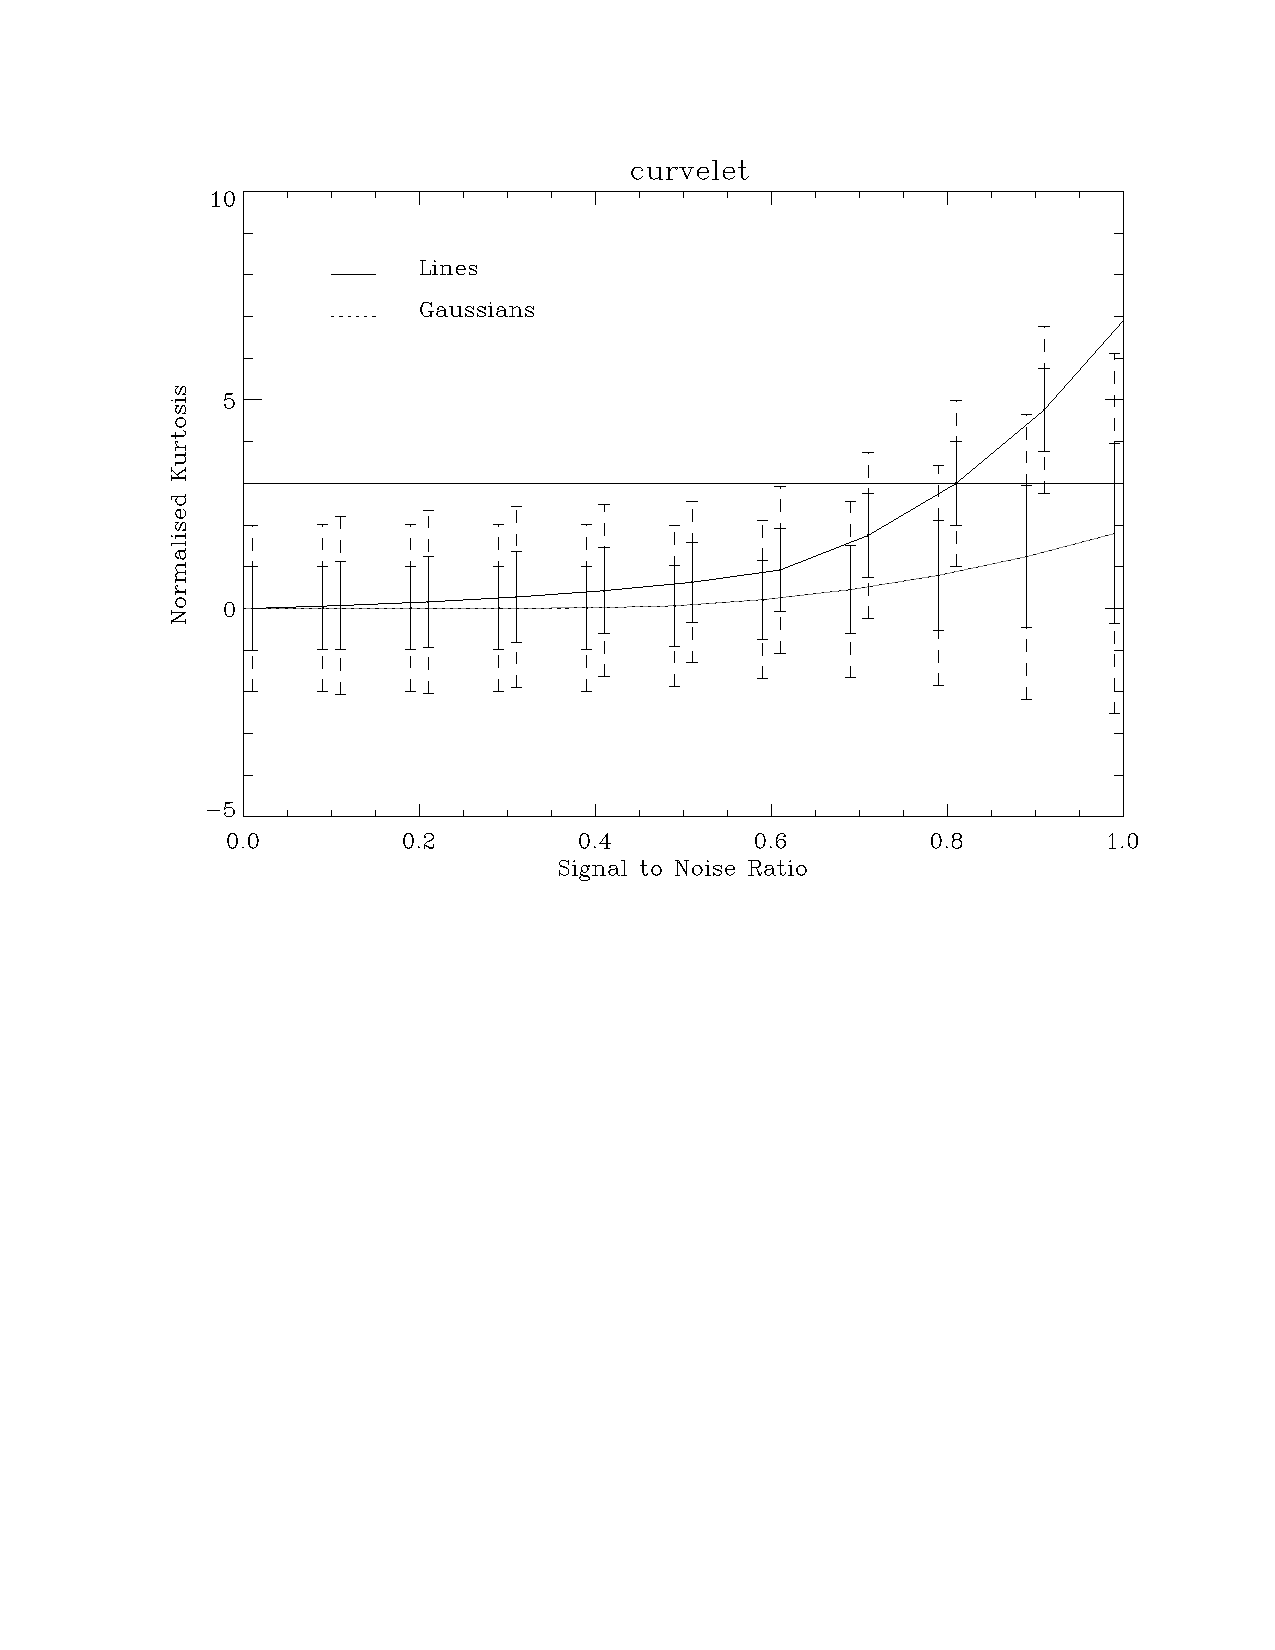
\includegraphics[trim= 2cm 13cm 2cm 3cm,width=7.9cm]{fig_sphere_cur_linedroite.pdf}
% \psfig{figure=fig_sphere_cur_linedroite.pdf,bbllx=2.5cm,bblly=12.5cm,bburx=19.5cm,bbury=25.5cm,width=8.5cm,height=6.5cm,clip=}
}}
\caption{Normalised kurtosis value versus the SNR for the wavelet coefficients (left) and the curvelet coefficients (right). 
The continuous error bars correspond to one $\sigma$ and the dashed error bars correspond to $2\sigma$.}
\label{fig_wtcur_sphere_linegauss}
\end{figure}

\section{Conclusions}
\index{wavelet!Kurtosis}
\index{wavelet!Higher Criticism}
\index{curvelet!Kurtosis}
\index{curvelet!Higher Criticism}
\index{SZ effect}
\index{cosmic strings}
\index{detection!non-Gaussianity}

The kurtosis of the wavelet coefficients is very often used in astronomy for the detection of non-Gaussianities in the CMB. It has been 
shown \citep{starck:sta03_1} that it is also possible to separate the non-Gaussian signatures associated with cosmic strings from those 
due to SZ effect by combining the excess kurtosis derived from these both the curvelet and the wavelet transform. It has been shown that 
kurtosis is asymptotically optimal in the class of weakly dependent symmetric non-Gaussian contamination with finite 8-th moments, while 
HC and MAX are asymptotically optimal in the class of weakly dependent symmetric non-Gaussian contamination with infinite 8-th moment \citep{starck:jin05}. 
Hence depending on the nature of the non-Gaussianity, a statitic is better than another one. This is a motivation for using several statistics 
rather than a single one for analysing CMB data. The case of the detection of cosmic string contaminations has been studied on simulated maps, 
and it has been shown that kurtosis outperforms clearly Max/HC \citep{starck:jin05}.  








\section{IDL Routines}
\label{ch_mrs_idl}
%\chapterhead{IDL Routines}
\markright{IDL Routines}

\subsection{Introduction}
A set of routines has been developed in IDL. Starting IDL using
the script program {\em mre} allows the user to get the multiresolution
environment, and all routines
described in the following can be called. An online help facility 
is also available by
invoking the {\em mrh} program under IDL.

\subsection{mw1d\_filter}
Filter a 1D signal by the the multiscale entropy.
{\bf
\begin{center}
     USAGE: mw1d\_filter, Signal, Result, Opt=Opt
\end{center}}
where 
\begin{itemize}
\item {\em Signal}: input  one-dimensional IDL array.
\item {\em Result}: output one-dimensional IDL array (filtered signal).
\item {\em Opt}:  string which contains the different options 
(see the {\em mw1d\_filter} C++  program).
\end{itemize}

\subsection{mw1d\_predict}
Considering a temporal signal $S$ with $n$ measures ($S[0..n-1]$), 
 {\em mr1d\_predict} estimates (or predicts) the next values $S[n .. n+dt]$.
A multiscale transformation is first applied, followed by filtering
in the wavelet space. At each scale, a predictor is then applied,
and the predicted signal is obtained from the reconstruction of
the predicted signal. 

{\bf
\begin{center}
     USAGE: Result = MW1D\_PREDICT(Signal,wave=wave,PredWave=PredWave,
                      NPredict=NPredict, Nscale=Nscale,  OPT=OPT, NCoef=NCoef)
\end{center}}
where 
\begin{itemize}
\item {\em wave}: output 2D IDL array; filtered wavelet coefficient
\item {\em PredWave}: output 2D IDL array; Predicted wavelet coefficient
\item {\em NPredict}: number of values to predict. Default is one.
\item {\em Nscale}: number of scales used for the wavelet transform
\item {\em NCoef:} Number of coefficients used for the prediction. Default is 3.
\item {\em OPT}: string which contains the differents options accepted by the
mw1d\_filter C++ program.
\end{itemize}

\subsection{mw\_filter}
Filter  an image by the multiscale entropy. 
This routine is calling the C++ executable {mw\_filter}. The keyword 
``OPT" allows 
all options described in the section corresponding to the 
 {\em mw\_filter} program.

{\bf
\begin{center}
     USAGE: mw\_filter, Data, FilterData, opt=opt
\end{center}}
{\em Data} is an image (2D IDL array), and {\em FilterData} is the result
of the filtering.

\subsection{mw\_deconv}
Deconvolve an image by  the  multiscale entropy. This routine calls 
the C++ executable {mw\_deconv}. The keyword ``OPT" 
allows 
all options described in the section corresponding to the 
 {\em mw\_deconv} program.

{\bf
\begin{center}
     USAGE: mw\_deconv, Data, PSF, DeconvData, opt=opt
\end{center}}
\subsubsection*{Examples:} 
\begin{itemize}
\item mw\_deconv, Imag, Psf, Result \\
deconvolve an image with all default options.
\item  mw\_deconv, Imag, Psf, Result, OPT='-i 30 -e 0'  \\
same example, but impose the number of iterations to be 30.
\end{itemize}

 



% \bibliographystyle{plain}
\bibliographystyle{astron}
\bibliography{ica,starck,wave,restore,ima,astro,mc,gauss,nab,curvelet,cluster,JLSBibTex}
\newpage
\addcontentsline{toc}{part}{Index}
\printindex

\clearpage


\newpage
\chapter*{Appendix A: The ``\`A Trous'' Wavelet Transform Algorithm}
\addcontentsline{toc}{chapter}{Appendix A: The ``\`A Trous'' Wavelet Transform Algorithm}

In a wavelet transform, a series of transformations of a signal is 
generated, providing a resolution-related set of  ``views'' of the signal.  
The properties satisfied by a wavelet transform, and in particular by the
{\it \`a trous} wavelet transform, are further discussed by Bijaoui et al. \cite{starck:bij94_1}. 
Extensive literature exists on the wavelet transform
and its applications (\cite{wave:daube88,wave:chui92,wave:ruskai92,starck:book98}). 
The discrete {\it \`a trous} algorithm is described in \cite{wave:hol89,wave:shensa92}.

We consider spectra, 
$\{c_0(k)\}$, defined as  the scalar product at 
samples $k$ of the function $f(x)$ with a scaling function $\phi(x)$
which corresponds to a low pass filter:
\begin{eqnarray}
c_0(k) = < f(x), \phi(x-k)>
\end{eqnarray}
The scaling function is chosen to satisfy the dilation equation:
\begin{eqnarray}
\frac{1}{2}\phi(\frac{x}{2}) = \sum_l h(l)\phi(x-l)
\end{eqnarray}
where $h$ is a discrete low-pass filter associated with the scaling function
$\phi$.  This means that a low-pass filtering
of the signal is, by definition, closely linked to another resolution level
of the signal.  The distance between levels increases by a factor 2 from one
scale to the next.


The smoothed data $c_j(k)$ at a given resolution $j$ and at a position
$k$  is the scalar product 

\begin{eqnarray}
c_j(k)= \frac{1}{2^j}< f(x), \phi(\frac{x-k}{2^j})>
\end{eqnarray}

This is consequently obtained by the convolution:
\begin{eqnarray}
c_j(k) = \sum_l h(l) \ \ c_{j-1} (k+2^{j-1}l)
\end{eqnarray}
The signal difference $w_j$ between two consecutive resolutions is:
\begin{eqnarray}
w_j(k) = c_{j-1}(k) - c_j(k) 
\end{eqnarray}
or:
\begin{eqnarray}
w_j(k) = \frac{1}{2^j}< f(x), \psi(\frac{x-k}{2^j})>  
\label{wj}
\end{eqnarray}
Here, the wavelet function $\psi$ is defined by:
\begin{eqnarray}
\frac{1}{2}\psi(\frac{x}{2})  = \phi(x) - \frac{1}{2}\phi(\frac{x}{2})
\end{eqnarray}

Equation~\ref{wj} defines the discrete wavelet transform, for a  
resolution level $j$.

For the scaling function, $\phi(x)$, the B-spline of degree 3 
was used in our calculations. As a filter we use 
$h = ( \frac{1}{16}, \frac{1}{4}, \frac{3}{8}, \frac{1}{4}, \frac{1}{16})$. 
See  Starck (1993)
for discussion of 
linear and other scaling functions.  Here  
we have derived a simple algorithm in order to compute the 
associated wavelet transform:
\begin{enumerate}
\item We initialize $j$ to 0 and we start with the data $c_j(k)$.
\item We increment $j$, and carry out a discrete convolution of the data
$c_{j-1}(k)$ using  the filter $h$. The distance between the central sample
and the adjacent ones is $2^{j-1}$.
\item After this smoothing, we obtain the discrete wavelet transform
from the difference $c_{j-1}(k) - c_j(k)$.
\item If $j$ is less than the number $p$ of resolutions we want to
compute, then we go to step 2.
\item The set ${\cal W} = \{ w_1, ..., w_p, c_p \}$ represents the
wavelet transform of the data.
\end{enumerate}

A series expansion of the original signal, $c_0$, 
in terms of
the wavelet coefficients is now given as follows. 
The final smoothed array $c_{p}(x)$ is added to all the differences $w_j$:
\begin{eqnarray}
c_0(k) = c_{p} + \sum_{j=1}^{p} w_j(k)
\label{eqn_rec}
\end{eqnarray}
 This equation provides a reconstruction formula for the original signal. At each scale $j$, we obtain a set $\{w_j\}$ which 
we call a wavelet scale.  The  wavelet scale 
has the same number of samples as the signal. 

% \chapter*{Appendix B: The Combined Filtering Method}
% \addcontentsline{toc}{chapter}{Appendix B:The Combined Filtering Method}

\chapter{The Combined Filtering Method}
 
In general, suppose that we are given $K$ linear transforms $T_1,
\ldots, T_K$ and let $\alpha_k$ be the coefficient sequence of an
object $x$ after applying the transform $T_k$, i.e. $\alpha_k = T_k
x$. We will assume that for each transform $T_k$ we have available a
reconstruction rule that we will denote by $T^{-1}_k$ although this is
clearly an abuse of notation.  Finally, $T$ will denote the block
diagonal matrix with the $T_k$'s as building blocks and $\alpha$ the
amalgamation of the $\alpha_k$'s.

A hard thresholding rule associated with the transform $T_k$ synthesizes 
an estimate $\tilde{s}_k$ via the formula 
\begin{equation}
\label{eq:ht}
\tilde{s}_k = T_k^{-1} \delta(\alpha_k)
\end{equation}
where $\delta$ is a rule that sets to zero all the coordinates of
$\alpha_k$ whose absolute value falls below a given sequence of
thresholds (such coordinates are said to be non-significant).
 
Given data $y$ of the form $y = s + \sigma z$, where $s$ is the image
we wish to recover and $z$ is standard white noise, we propose solving
the following optimization problem \cite{starck:spie01a}:
\begin{equation}
  \label{eq:l1-min}
  \min \|T\tilde{s}\|_{\ell_1}, \quad \mbox{subject to} \quad s \in C,  
\end{equation}
where $C$ is the set of vectors $\tilde{s}$ 
which obey the linear constraints
\begin{equation}
\label{eq:constraints}
\left\{  \begin{array}{ll}
  \tilde{s} \ge 0, \\
  |T\tilde{s} - Ty| \le e; 
  \end{array}
  \right. 
\end{equation}
here, the second inequality constraint 
only concerns the set of significant coefficients, 
i.e. those indices $\mu$ such that $\alpha_\mu =
(Ty)_\mu$ exceeds (in absolute value) a threshold $t_\mu$. Given a
vector of tolerance $(e_\mu)$, we seek a solution whose coefficients
  $(T\tilde{s})_\mu$ are within $e_\mu$ of the noisy
empirical $\alpha_\mu$'s.  Think of $\alpha_\mu$ as being given by
\[
y = \langle y, \varphi_\mu \rangle, 
\]
so that $\alpha_\mu$ is normally distributed with mean $\langle f,
\varphi_\mu \rangle$ and variance $\sigma^2_\mu = \sigma^2
\|\varphi_\mu\|^2_2$. In practice, the threshold values range
typically between three and four times the noise level $\sigma_\mu$
and in our experiments we will put $e_\mu = \sigma_\mu/2$. In short,
our constraints guarantee that the reconstruction will take into
account any pattern which is detected as significant by  any of the
$K$ transforms.
   
\subsubsection*{The Minimization Method}

We propose solving (\ref{eq:l1-min}) using the method of hybrid
steepest descent (HSD) \cite{wave:yamada01}. HSD consists of building
the sequence
\begin{eqnarray}
 s^{n+1} = P(s^{n}) - \lambda_{n+1} \nabla_J(P(s^{n})); 
\end{eqnarray}
Here, $P$ is the $\ell_2$ projection operator onto the feasible set
$C$, $\nabla_J$ is the gradient of equation~\ref{eq:l1-min}, and
$(\lambda_{n})_{n \ge 1}$ is a sequence obeying $(\lambda_{n})_{n\ge
  1} \in [0,1] $ and $\lim_{ n \rightarrow + \infty } \lambda_{n} = 0$.

The combined filtering algorithm is:
\begin{enumerate}
\baselineskip=0.4truecm
\itemsep=0.1truecm
\item Initialize $L_{\max} = 1$, the number of iterations $N_i$, and
  $\delta_{\lambda} = \frac{L_{\max}}{N_i}$.
\item Estimate the noise standard deviation $\sigma$, and set $e_k =
  \frac{\sigma}{2}$.
\item For k = 1, .., $K$ calculate the transform: $\alpha^{(s)}_k
  = T_k s$.
\item Set $\lambda = L_{\max}$, $n = 0$, and $\tilde s^{n}$ to 0.
\item While $\lambda >= 0$ do
\begin{itemize}
\item $u = \tilde s^{n}$.
\item For k = 1, .., $K$ do
  \begin{itemize}
  \item Calculate the transform $\alpha_{k} = T_k u$.
  \item For all coefficients $\alpha_{k,l}$ do
     \begin{itemize}
     \item Calculate the residual $r_{k,l} = \alpha^{(s)}_{k,l} -
       \alpha_{k,l}$
       
     \item if $\alpha^{(s)}_{k,l}$ is significant and $ \mid r_{k,l}
       \mid > e_{k,l}$ then $\alpha_{k,l} = \alpha^{(s)}_{k,l}$
     \item $\alpha_{k,l} = sgn(\alpha_{k,l}) ( \mid \alpha_{k,l} \mid - \lambda)_{+}$.
     \end{itemize}
   \item $u = T_k^{-1} \alpha_{k}$
  \end{itemize}
\item Threshold negative values in $u$ and $\tilde s^{n+1} = u$.
\item $n = n + 1$, $\lambda = \lambda - \delta_{\lambda} $, and goto 5.
\end{itemize}
\end{enumerate}
 

 
\end{document}
